\documentclass[11pt, a4paper]{article}
%\usepackage{proj1}
\usepackage{natbib}
\usepackage{fancyhdr}  
\usepackage{subcaption}
\usepackage{caption}
\usepackage{graphicx}
\usepackage[autolanguage,nosepfour]{numprint}
\usepackage{multirow}
\linespread{1.25} 
\setlength{\parindent}{0cm}
\graphicspath{{Images/}}
\usepackage{hyperref}
\usepackage{amsmath}
\usepackage{amsfonts}
\usepackage{amssymb}
\usepackage{amsthm}
\usepackage{mathtools}
\usepackage{commath}
\usepackage{bbm}
\usepackage[ruled,vlined]{algorithm2e}

%\usepackage[sc,osf]{mathpazo}
\usepackage{subcaption}
\usepackage[a4paper, top=1in, left=1.0in, right=1.0in, bottom=1in, includehead, includefoot]{geometry} %Usually have top as 1in

\usepackage{listings}
\usepackage{color} %red, green, blue, yellow, cyan, magenta, black, white
\definecolor{mygreen}{RGB}{28,172,0} % color values Red, Green, Blue
\definecolor{mylilas}{RGB}{170,55,241}


\hypersetup{colorlinks,linkcolor={black},citecolor={blue},urlcolor={black}}
\usepackage{color}
\urlstyle{same}


\theoremstyle{definition}
\newtheorem{definition}{Definition}[section]

\newcommand{\adja}{q_a}
\newcommand{\adjb}{q_b}
\newcommand{\adjaB}{q_{a,\partial \Omega}}
\newcommand{\adjbB}{q_{b,\partial \Omega}}
\newcommand{\adjB}{q_{\partial \Omega}}
\newcommand{\Adja}{\mathbf{p}}
\newcommand{\Adjb}{q}
\newcommand{\adj}{q}
\newcommand{\Adjc}{{q}_{\partial \Omega}}
\newcommand{\ra}{\rho_a}
\newcommand{\rb}{\rho_b}
\newcommand{\w}{\mathbf{w}}
\newcommand{\f}{\mathbf{f}}
\newcommand{\ve}{\mathbf{v}}
\newcommand{\n}{\mathbf{n}}
\newcommand{\h}{\mathbf{h}}
\newcommand{\K}{\mathbf{K}}
\newcommand{\hr}{\widehat \rho}
\newcommand{\jf}{\mathbf j}

\DeclareMathOperator{\sgn}{sgn}
\DeclareMathOperator{\Grad}{Grad}
\DeclareMathOperator{\Div}{Div}
\DeclareMathOperator{\Lap}{Lap}

%	\begin{figure}[h]
%		\centering
%		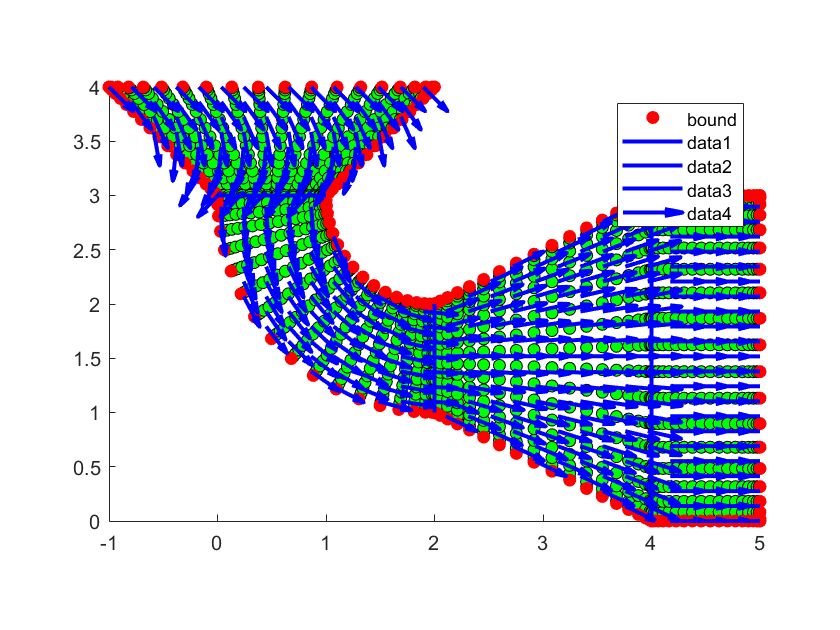
\includegraphics[scale=0.35]{F1.png}
%		\caption{Forward $\rho$ for $a = 0.01$} 
%		\label{F1}
%	\end{figure}

\begin{document}
	
\section{Quick Questions/Comments}
When does the mean field approximation hold? High density limit but then issues in clusters?\\
ALOP workshop	\\
Did the normal plots - look nice\\
fixed tables in document\\
did table on $\theta$ vs $r$ varied differently for interpolation\\
\\
Presentation:\\
Other things on motivation slide?\\
Other example? Paper one with external potential? Or multishape?
\section{Polar Derivatives}
In order to compute the gradient, divergence and Laplacian we have to use the standard definition of the polar versions to derive these. For $ r \neq 0$ we get
\begin{align*}
	\Grad  &= \left(D_r, \frac{1}{r} D_\theta\right) ,\\
	\Div &= \left(D_r + \frac{1}{r}, \frac{1}{r} D_\theta\right)^\top ,\\
	\Lap  &= D_{rr} +\frac{1}{r}D_r +  \frac{1}{r^2} D_{\theta \theta}.
\end{align*}
At $ r = 0$, we need to treat these operators more carefully. We know that $\frac{1}{r} D_\theta = D_{r\theta}$, since $D_\theta =0$ at $r = 0$, and so $ \Grad = \left(D_r, D_{r\theta}\right)$. Similarly, at $r = 0$, we get that $\Div = \left(2D_r, D_{r\theta}\right)^\top$. Finally we have that $\Lap = 2 D_{rr} + \frac{1}{2} D_{\theta\theta}D_{rr}$ at the origin. \\
\\
If we assume that $D_\theta =0$, then for $\frac{1}{r} D_\theta = D_{r\theta}$ to hold we can use L'Hopital's rule. 
However, why can we use this for $D_r + \frac{1}{r} = 2D_r$ ? And why is $D_\theta =0$? And we also assume $D_{\theta \theta}=0$ in the Laplacian if we apply this rule. 

\section{Simple OCP} \label{sec:SimpleOCP}
(note: MSSimpleOCP in code)
The first problem we consider is a simple optimal control problem with no external potential or flow, using the overdamped DDFT with Gaussian pair potential. We are interested in the following two setups. We first run a forward problem with attractive particles and diffusion, which builts clusters. Then we set this as the desired state for an optimal control problem where the problem setup includes repulsive particles and diffusion. The question is then how expensive it is to recreate the clusters built from attraction with repulsive particles. 
In a second example we set the forward problem with repulsive particles as the $\hr$ and the forward problem with attractive particles becomes the starting point for the optimal control problem.
We can then ask which of these two scenarios has a higher cost associated to it after optimization. 
The initial condition for $\rho$ is uniform $\rho_0 = 0.1$ in a box of dimensions $[0,10]^2$ with $N = 30$. The time horizon is $90,3)$, with $n = 30$. The interaction strengths are $\kappa = -2$ and $\kappa = 2$. The ODE tolerances are $10^{-8}$ and the optimality tolerances are $10^{-3}$. The regularization parameter is set to $\beta = 10^{-3}$ and $\lambda = 0.01$ for stability.
\\
In order to gauge which of the two examples will be harder to solve, we compute the distance between $\rho$ with $\kappa = 0$ and $\hr$ a forward problem with $\kappa = -2$. This corresponds to computing $\mathcal J_{FW}$ for such a problem. $\mathcal J_{FW}  = 0.0101$. We can compute the same for $\hr$ with $\kappa = 2$ and get $\mathcal J_{FW} = 0.0065$. This shows that the non-interacting particle dynamics is closer to the repulsive dynamics than to the attractive dynamics. 
\\
\\

We fist consider the example in which the dynamics includes repulsive particle interactions. We are interested in how well the optimal control solution can match a $\hr$, which is created by dynamics with attractive particles. The result can be seen in Figures \ref{FSc} and \ref{FSd}. The uncontrolled cost is $\mathcal J_{FW} = 0.0323$ and the optimal cost is $\mathcal J_{Opt} =  0.0098$. In the second example we consider attractive particle dynamics, which are controlled to mimic a repulsive dynamic. The result can be seen in Figures \ref{FSa} and \ref{FSb}. The uncontrolled cost is $\mathcal J_{FW} = 0.0323$ and the optimal cost is $\mathcal J_{Opt} =  0.0078$.
	

	\begin{figure}[h]
		\centering
		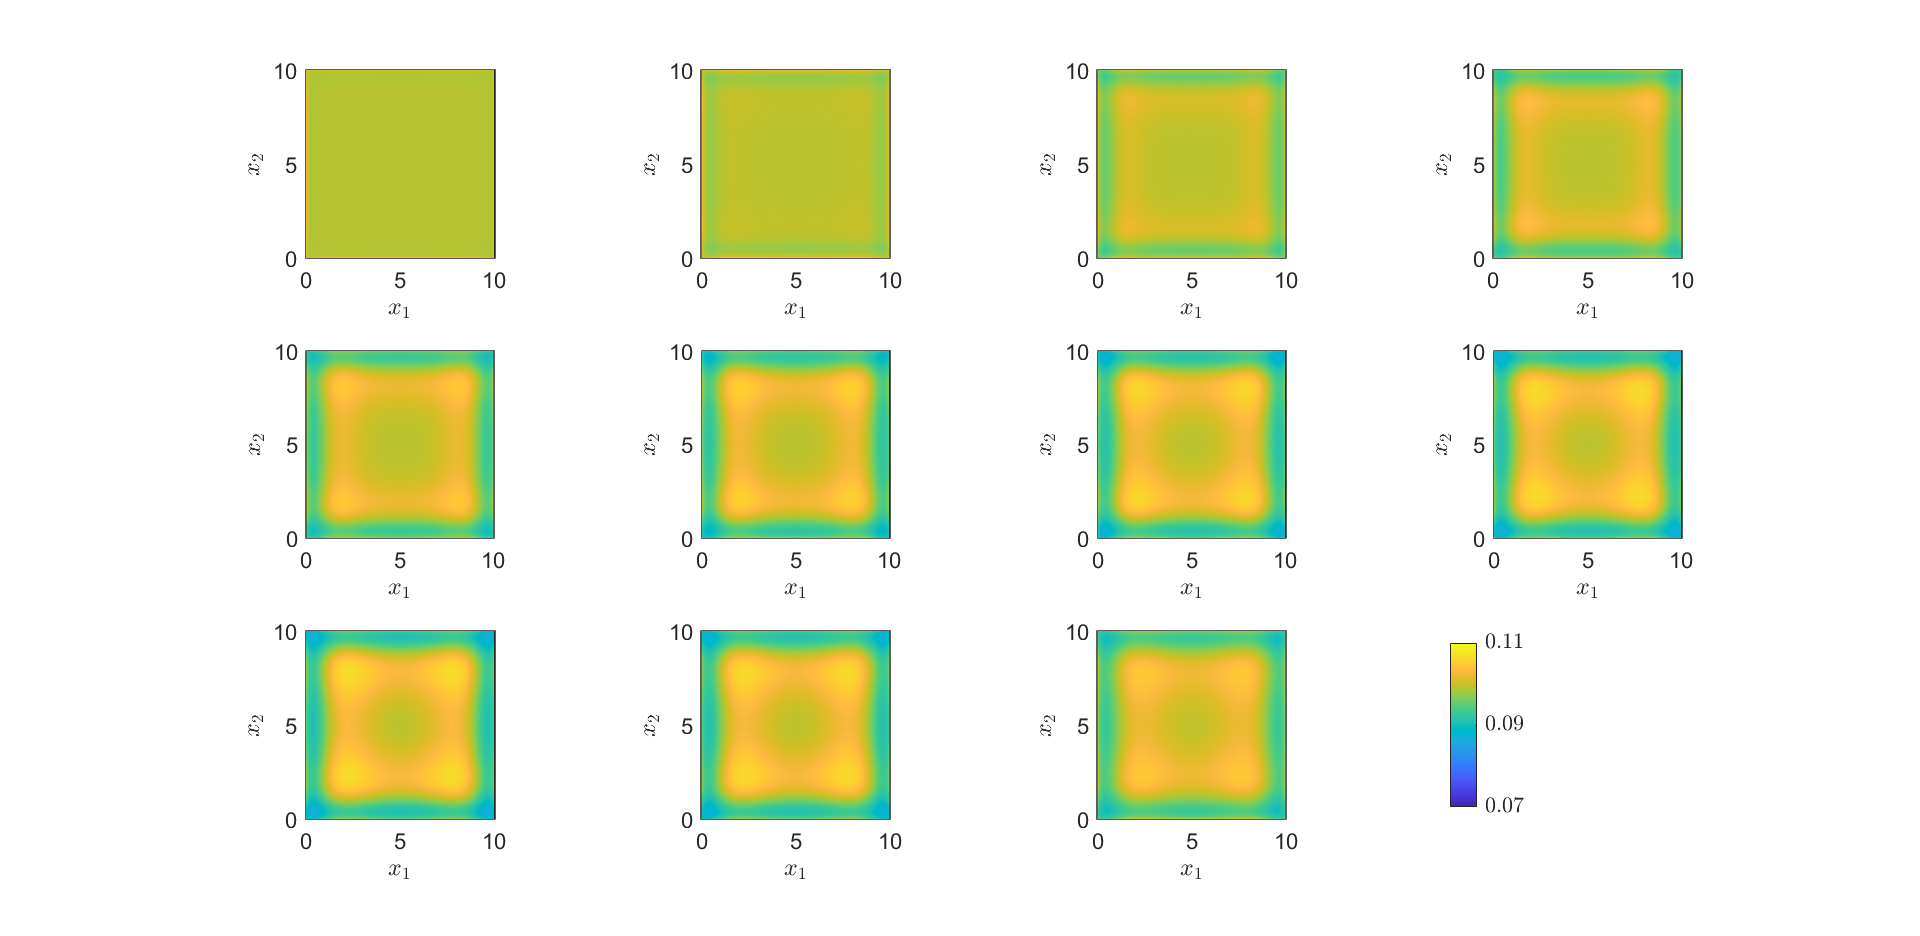
\includegraphics[scale=0.35]{Simplerhok.png}
		\caption{Examples Section \ref{sec:SimpleOCP}: Optimal $\rho$ for $\kappa = 2$.} 
		\label{FSc}
	\end{figure}
	\begin{figure}[h]
		\centering
		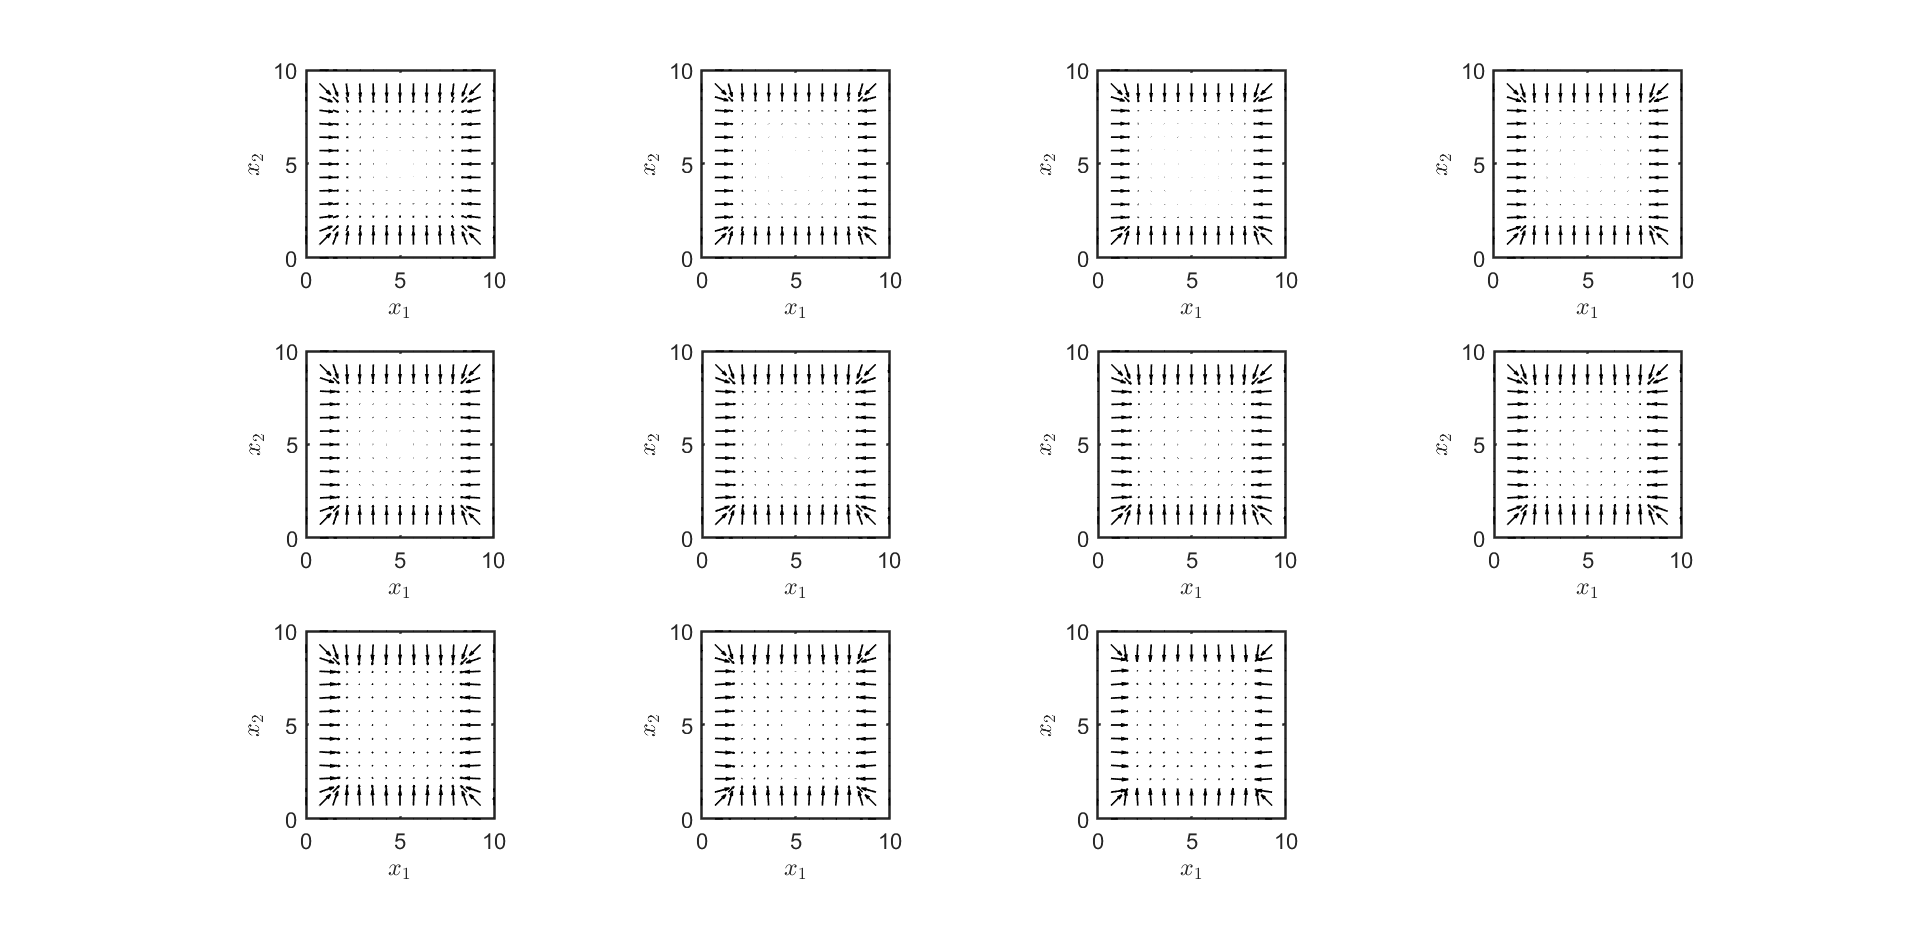
\includegraphics[scale=0.35]{SimpleConk.png}
		\caption{Examples Section \ref{sec:SimpleOCP}: Optimal Control for $\kappa = 2$.} 
		\label{FSd}
	\end{figure}

	\begin{figure}[h]
		\centering
		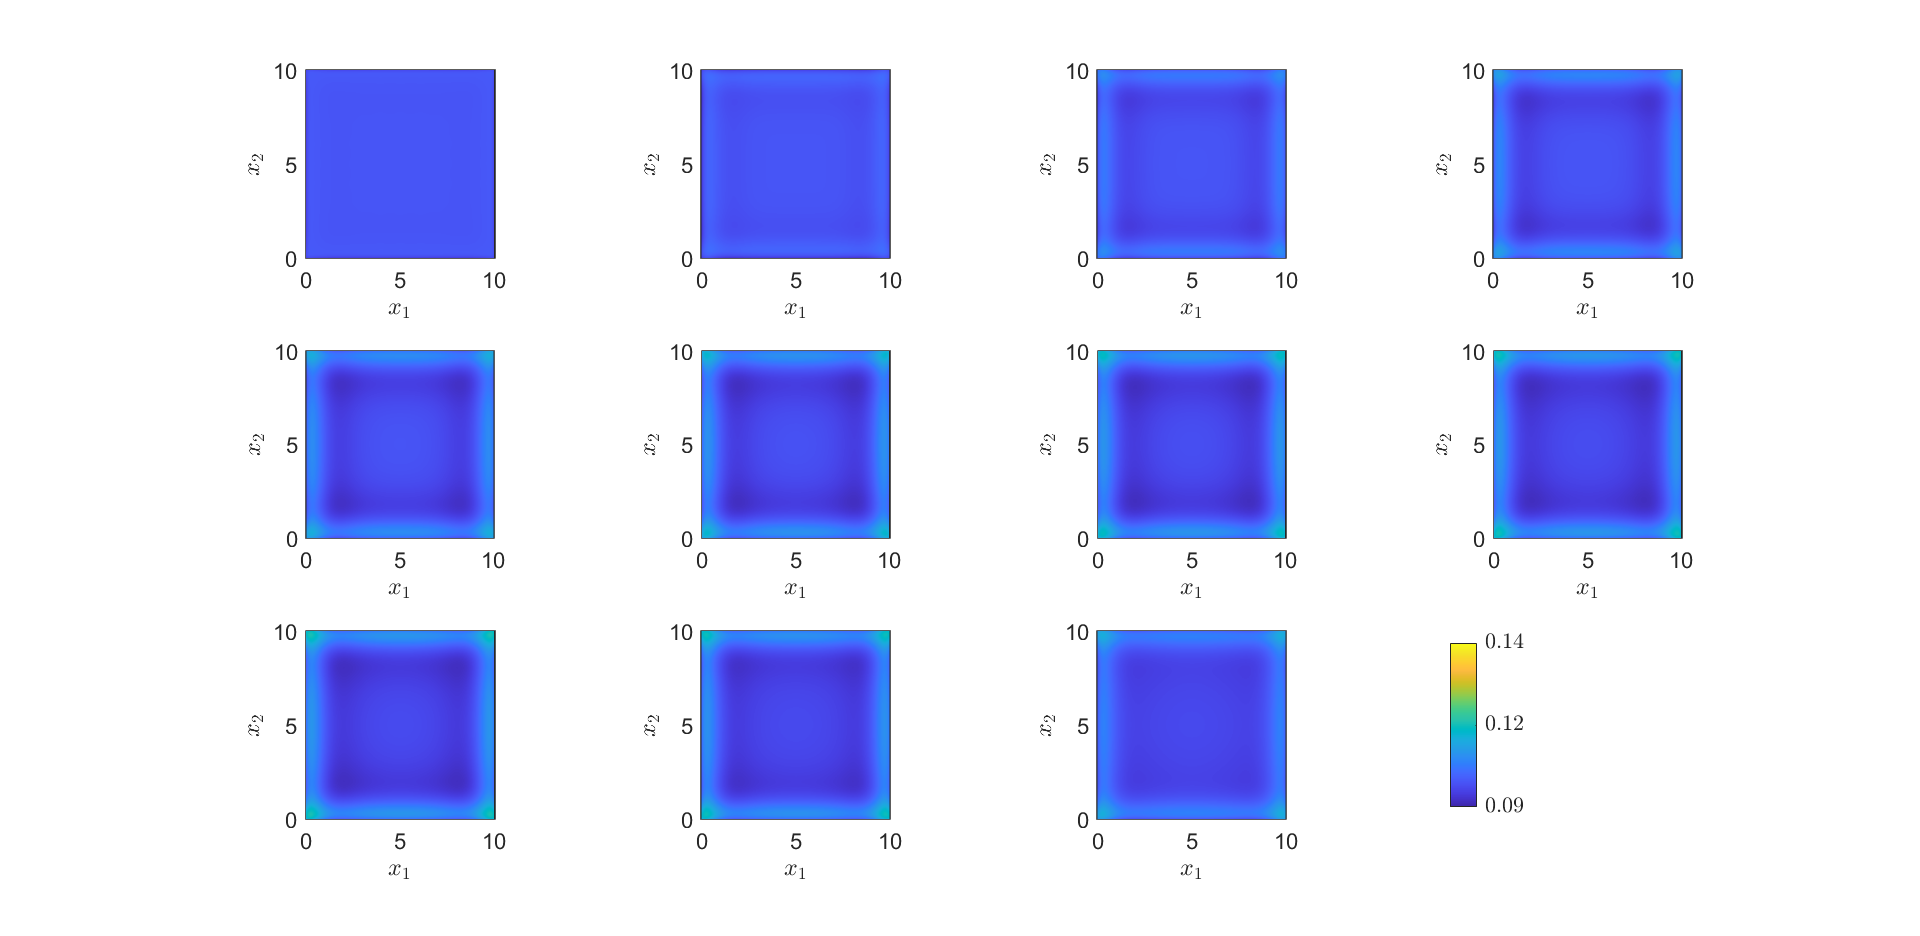
\includegraphics[scale=0.35]{Simplerhokn.png}
		\caption{Examples Section \ref{sec:SimpleOCP}: Optimal $\rho$ for $\kappa = -2$.} 
		\label{FSa}
	\end{figure}
	\begin{figure}[h]
		\centering
		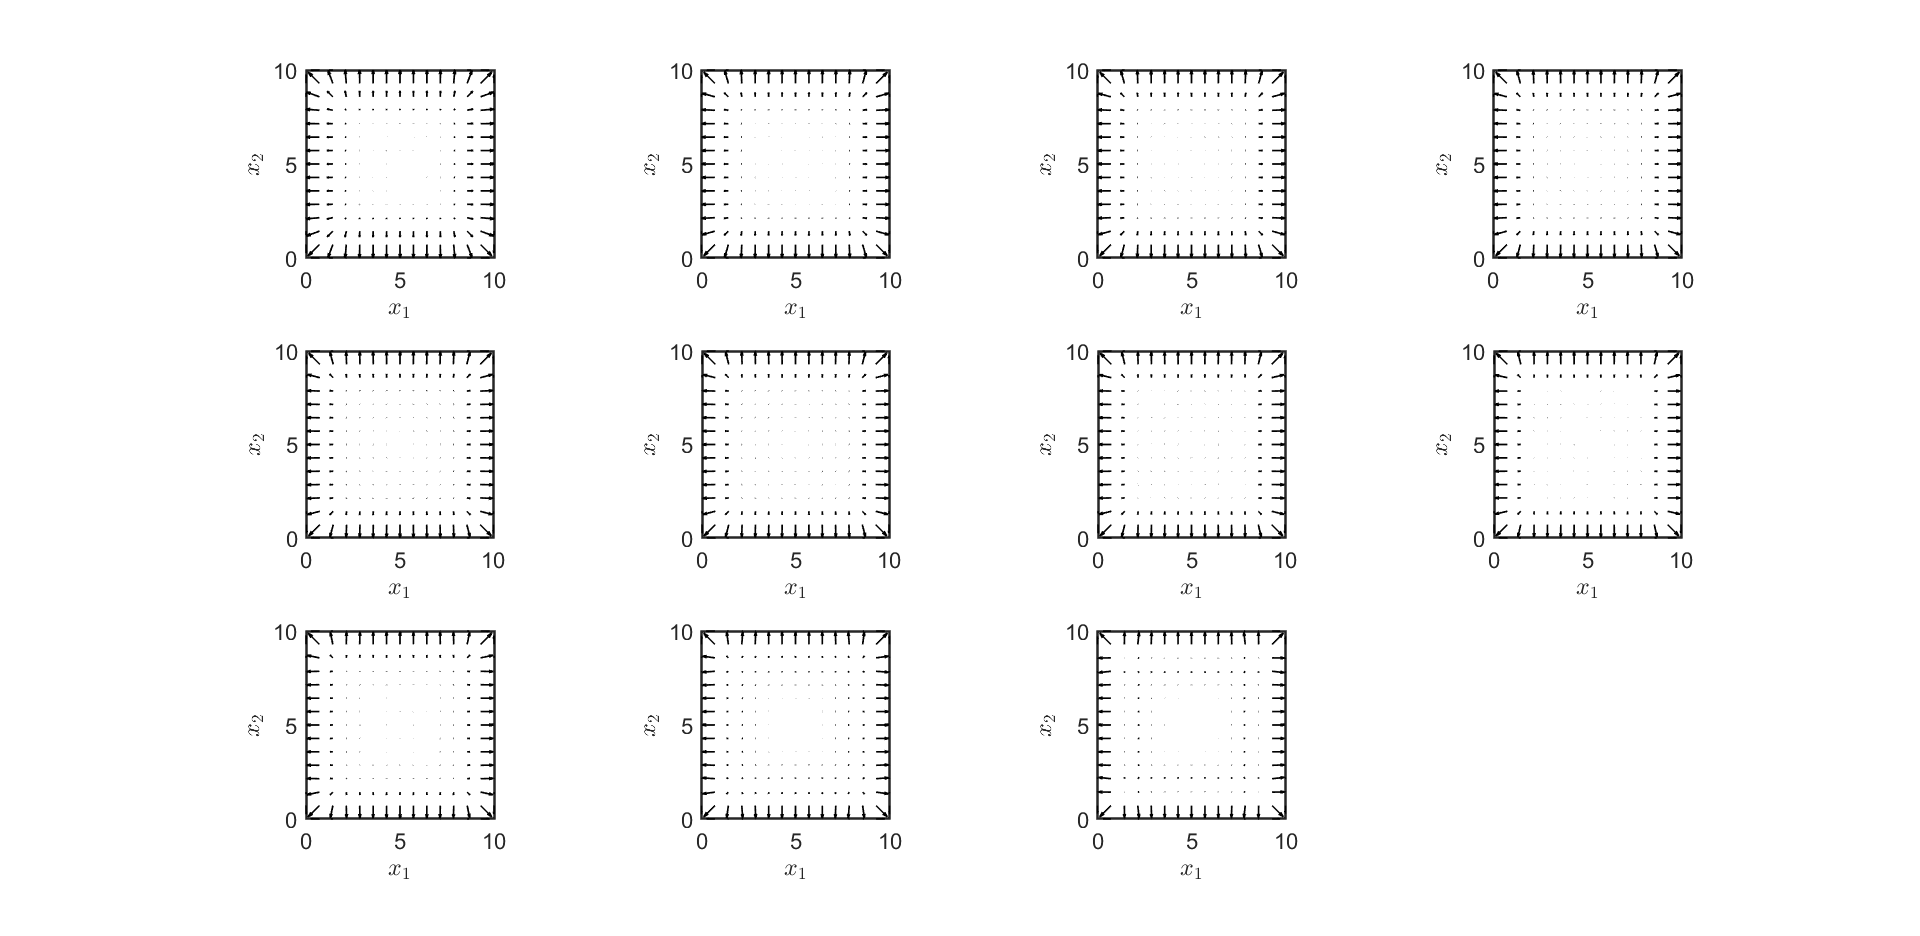
\includegraphics[scale=0.35]{SimpleConkn.png}
		\caption{Examples Section \ref{sec:SimpleOCP}: Optimal Control for $\kappa = -2$.} 
		\label{FSb}
	\end{figure}
	

\section{Varying External Potential} \label{sec:VaryExPotential}
+++ Add plot of $V_{ex}$ vs optimal control +++
(Note: MSSeparationOCP in code)
We consider the overdamped DDFT with no flux boundary conditions, a Gaussian pair potential and for the forward problem, no background flow. 
The external potential is given by
\begin{align*}
	V_{ext} = 0.03 \cos(2\pi (t + 0.5)/2.75)r^2,
\end{align*}
see Figure \ref{F1}. The time horizon for the problem is $(0,3)$ with $n = 30$ and the spatial domain is a box of dimension $[-5,5]^2$ with $N = 30$. The initial condition for $\rho$ is the uniform distribution $\rho_0 = 0.1$. The ODE tolerances are set to be $10^{-8}$. All figures show the time points $2,\  5,\ 8,\  10,\ 12,\ 14,\ 16,\ 18,\ 20,\ 23,\ 26$ out of $30$.
While Figure \ref{F0c} shows the effect of $V_{ext}$ in absence of the interaction term, Figures \ref{F0a} and \ref{F0b} show the effect of the positive and negative attraction term in absence of the external potential. We note that the change in $\rho$ by these interactions is of the same magnitude as the effect of $V_{ext}$. In Figures \ref{F2a} and \ref{F2b} the effects of $V_{ext}$ in combination with the two different interaction potentials are shown. 
\\
\\
These forward problems are now used in the context of an optimal control problem. We are interested in optimizing a system without external potential present to mimic those with the chosen external potential. Therefore, we first set $\hr$ to be the forward problem without particle interactions ($\kappa =0$) and with the external potential, see Figure \ref{F0c}. We then start the optimization by choosing the same uniform initial condition for $\rho$ but without an external potential. The intitial guess for $\w$ is zero. We then expect $\w$ to mimic the external potential, forcing particles in the desired state and it is of interest in what way this flow control is similar to the external potential that shaped $\hr$.
The same experiment is conducted with repulsive particles ($\kappa = 2$), where Figure \ref{F2a} shows the desired state and Figure \ref{F0a} displays the uncontrolled, initial state for the optimization. Then for attractive particles ($\kappa = -2$) we have that $\hr$ takes the form shown in Figure \ref{F2b}, while the uncontrolled profile of $\rho$ is displayed in Figure \ref{F0b}.\\
\\
We choose $\lambda = 0.01$ and the optimality tolerances are $10^{-3}$ and the regularization parameter is set to $\beta = 10^{-3}$. 
\begin{figure}[h]
	\centering
	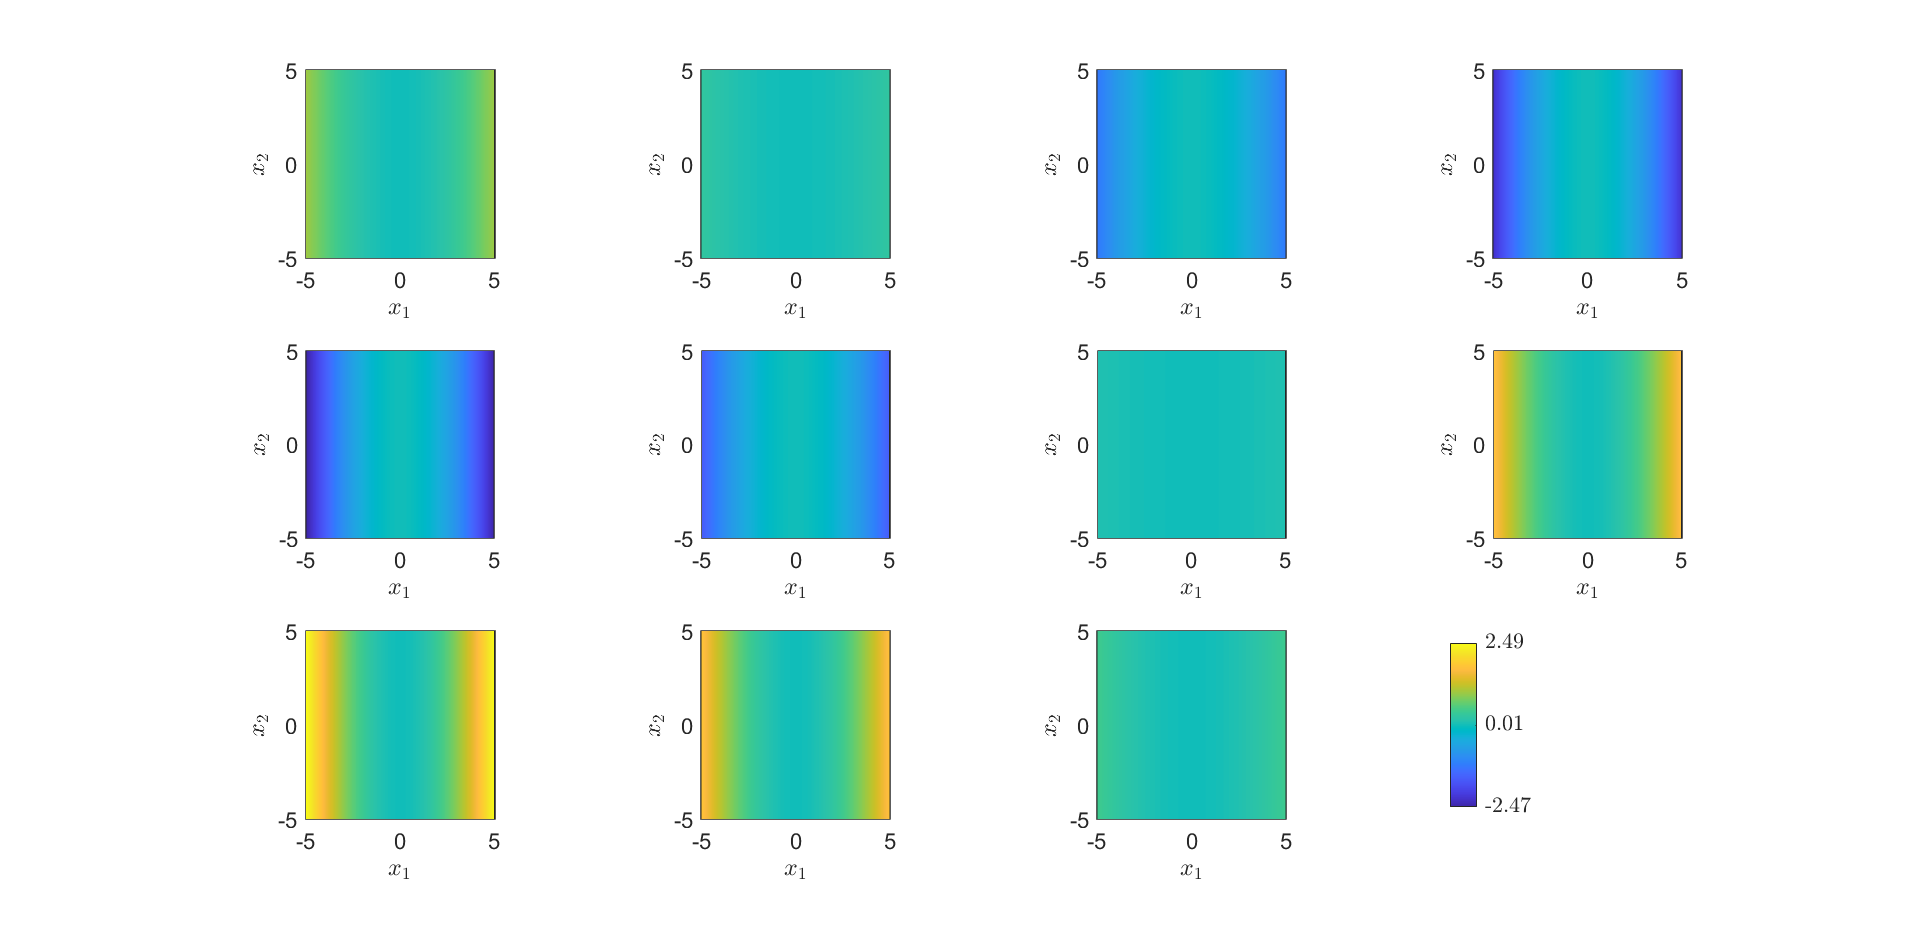
\includegraphics[scale=0.35]{Vext.png}
	\caption{Examples Section \ref{sec:VaryExPotential}: External potential over time.} 
	\label{F1}
\end{figure}
\begin{figure}[h]
	\centering
	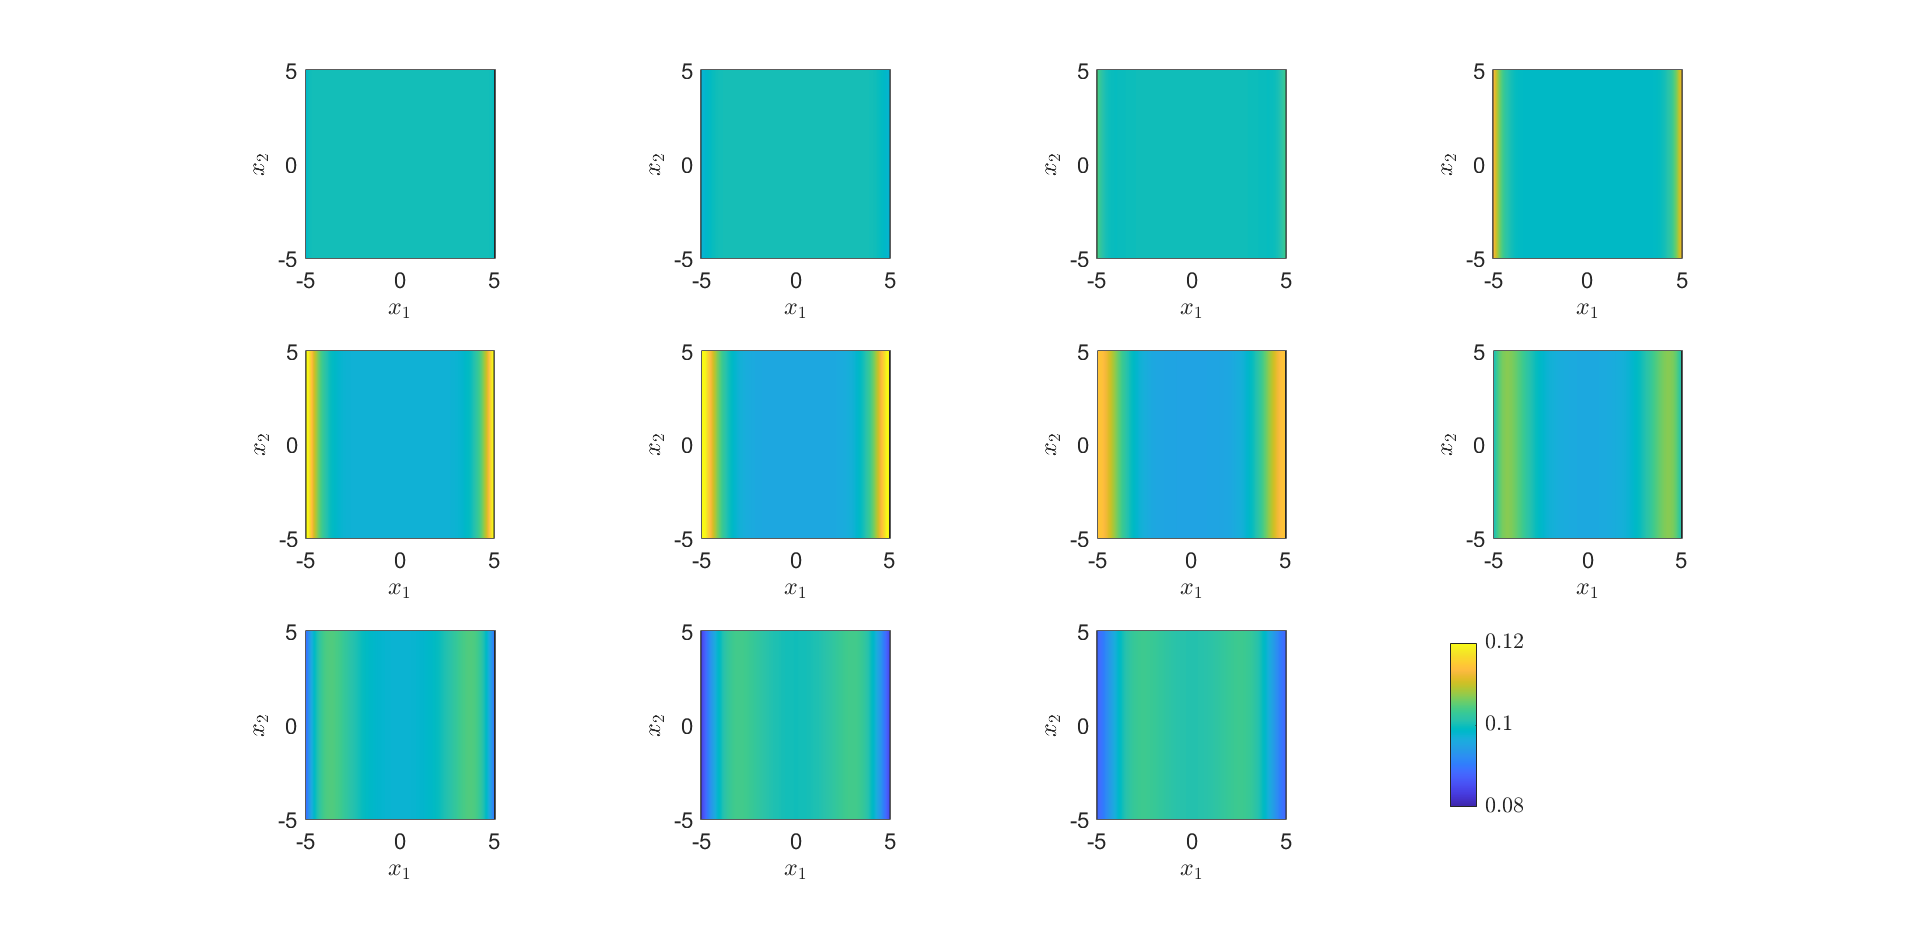
\includegraphics[scale=0.35]{rhok0V.png}
	\caption{Examples Section \ref{sec:VaryExPotential}: Forward $\rho$ over time horizon, $\kappa = 0$, $V_{ext}$ on. This is the desired state $\hr$ for the uncontrolled particle distribution without interactions, which is a uniform distribution.} 
	\label{F0c}
\end{figure}
\begin{figure}[h]
	\centering
	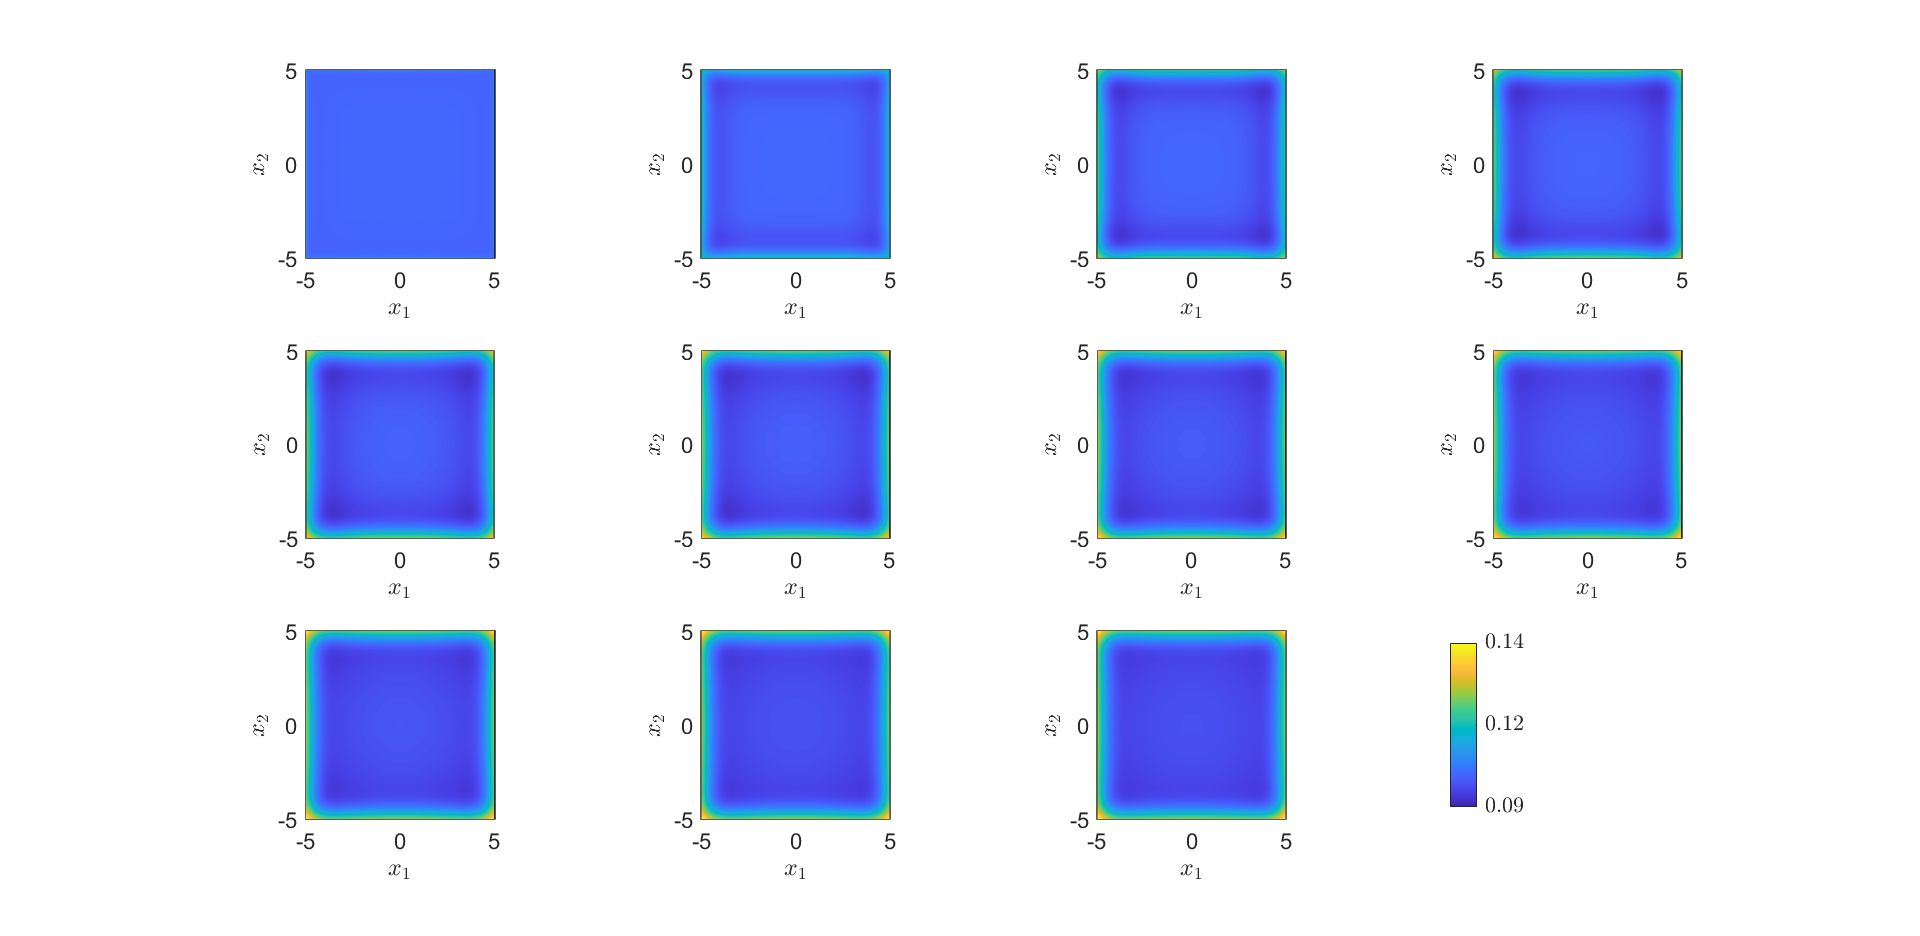
\includegraphics[scale=0.35]{rhok05.png}
	\caption{Examples Section \ref{sec:VaryExPotential}: Forward $\rho$ over time horizon, $\kappa = 2$, $V_{ext}$ off. This is the uncontrolled state corresponding to the desired state $\hr$ displayed in Figure \ref{F2a}.} 
	\label{F0a}
\end{figure}
\begin{figure}[h]
	\centering
	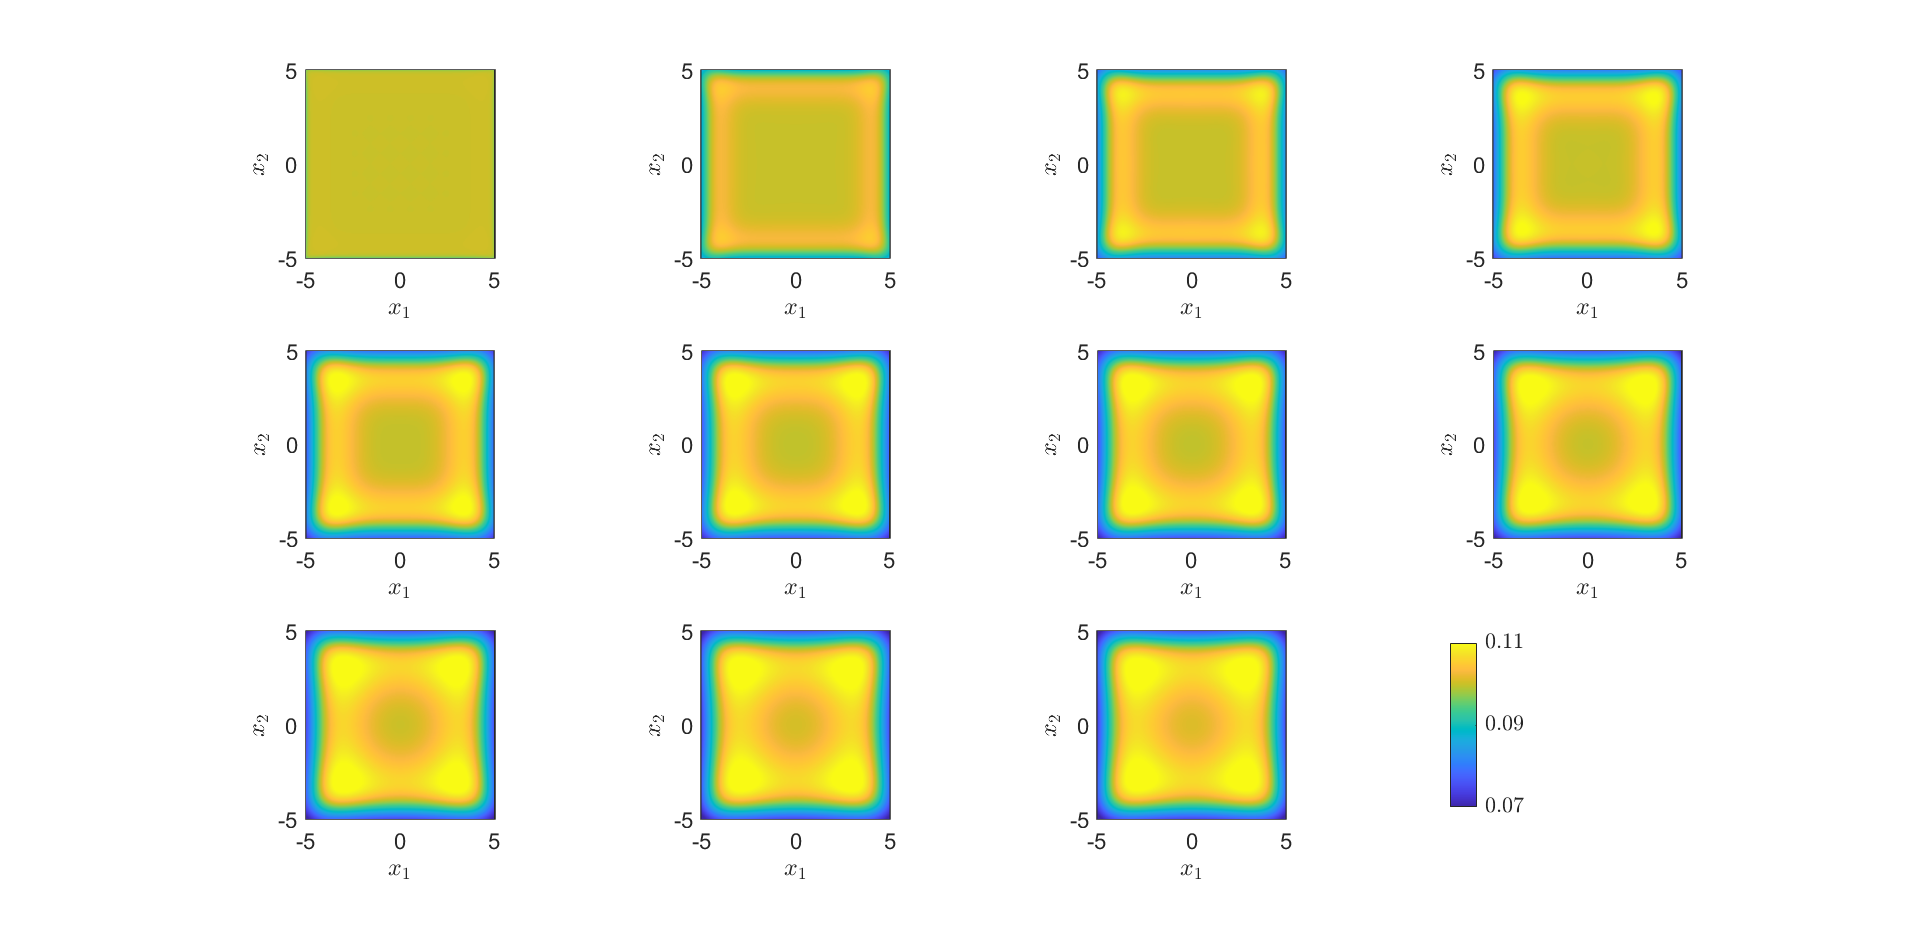
\includegraphics[scale=0.35]{rhokn05.png}
	\caption{Examples Section \ref{sec:VaryExPotential}: Forward $\rho$ over time horizon, $\kappa = - 2$, $V_{ext}$ off. This is the uncontrolled state corresponding to the desired state $\hr$ displayed in Figure \ref{F2b}.} 
	\label{F0b}
\end{figure}



\begin{figure}[h]
	\centering
	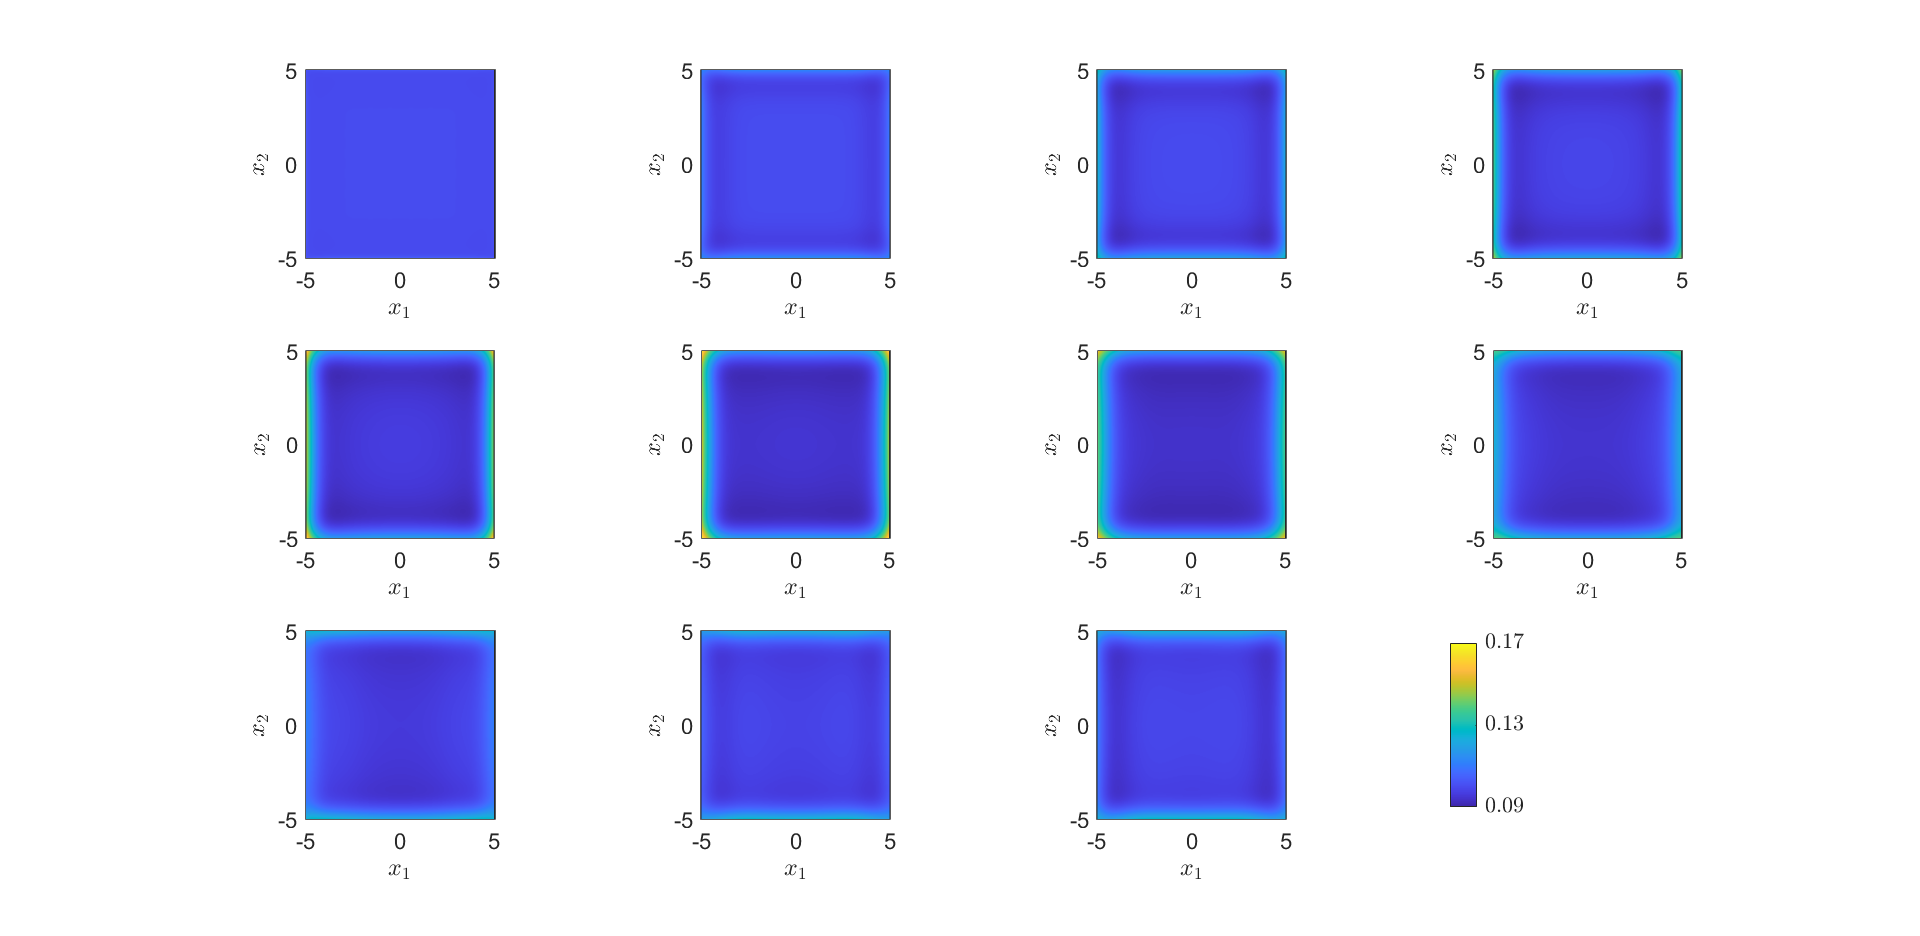
\includegraphics[scale=0.35]{rhok05V.png}
	\caption{Examples Section \ref{sec:VaryExPotential}: Forward $\rho$ over time horizon, $\kappa = 2$, $V_{ext}$ on. This is the desired state $\hr$ for the uncontrolled particle distribution shown in Figure \ref{F0a}.} 
	\label{F2a}
\end{figure}
\begin{figure}[h]
	\centering
	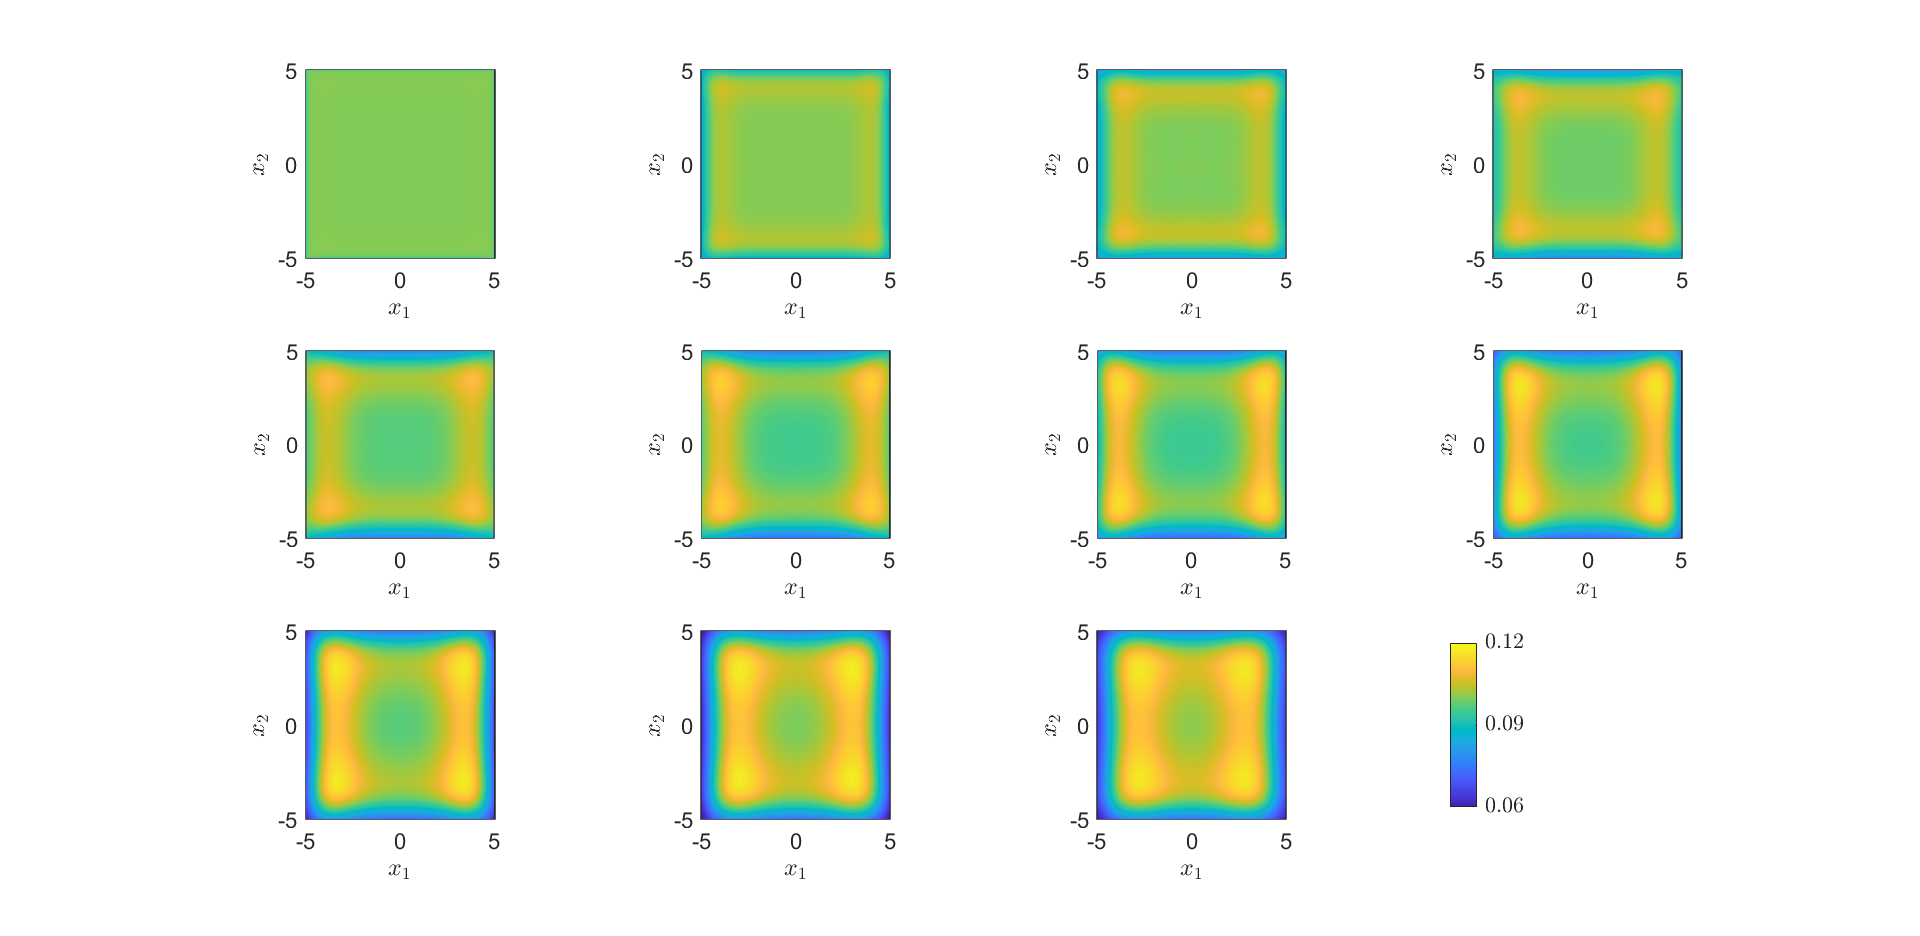
\includegraphics[scale=0.35]{rhokn05V.png}
	\caption{Examples Section \ref{sec:VaryExPotential}: Forward $\rho$ over time horizon, $\kappa = - 2$, $V_{ext}$ on. This is the desired state $\hr$ for the uncontrolled particle distribution shown in Figure \ref{F0b}.} 
	\label{F2b}
\end{figure}

At first we set $\hr$ to be as defined in Figure \ref{F0c}. The uncontrolled state here is simply a uniform distribution. We get that $\mathcal J_{FW} = 0.0029$ and $J_{Opt} = 0.0010$. The results can be seen in Figure \ref{F3a} and \ref{F3b}.

\begin{figure}[h]
	\centering
	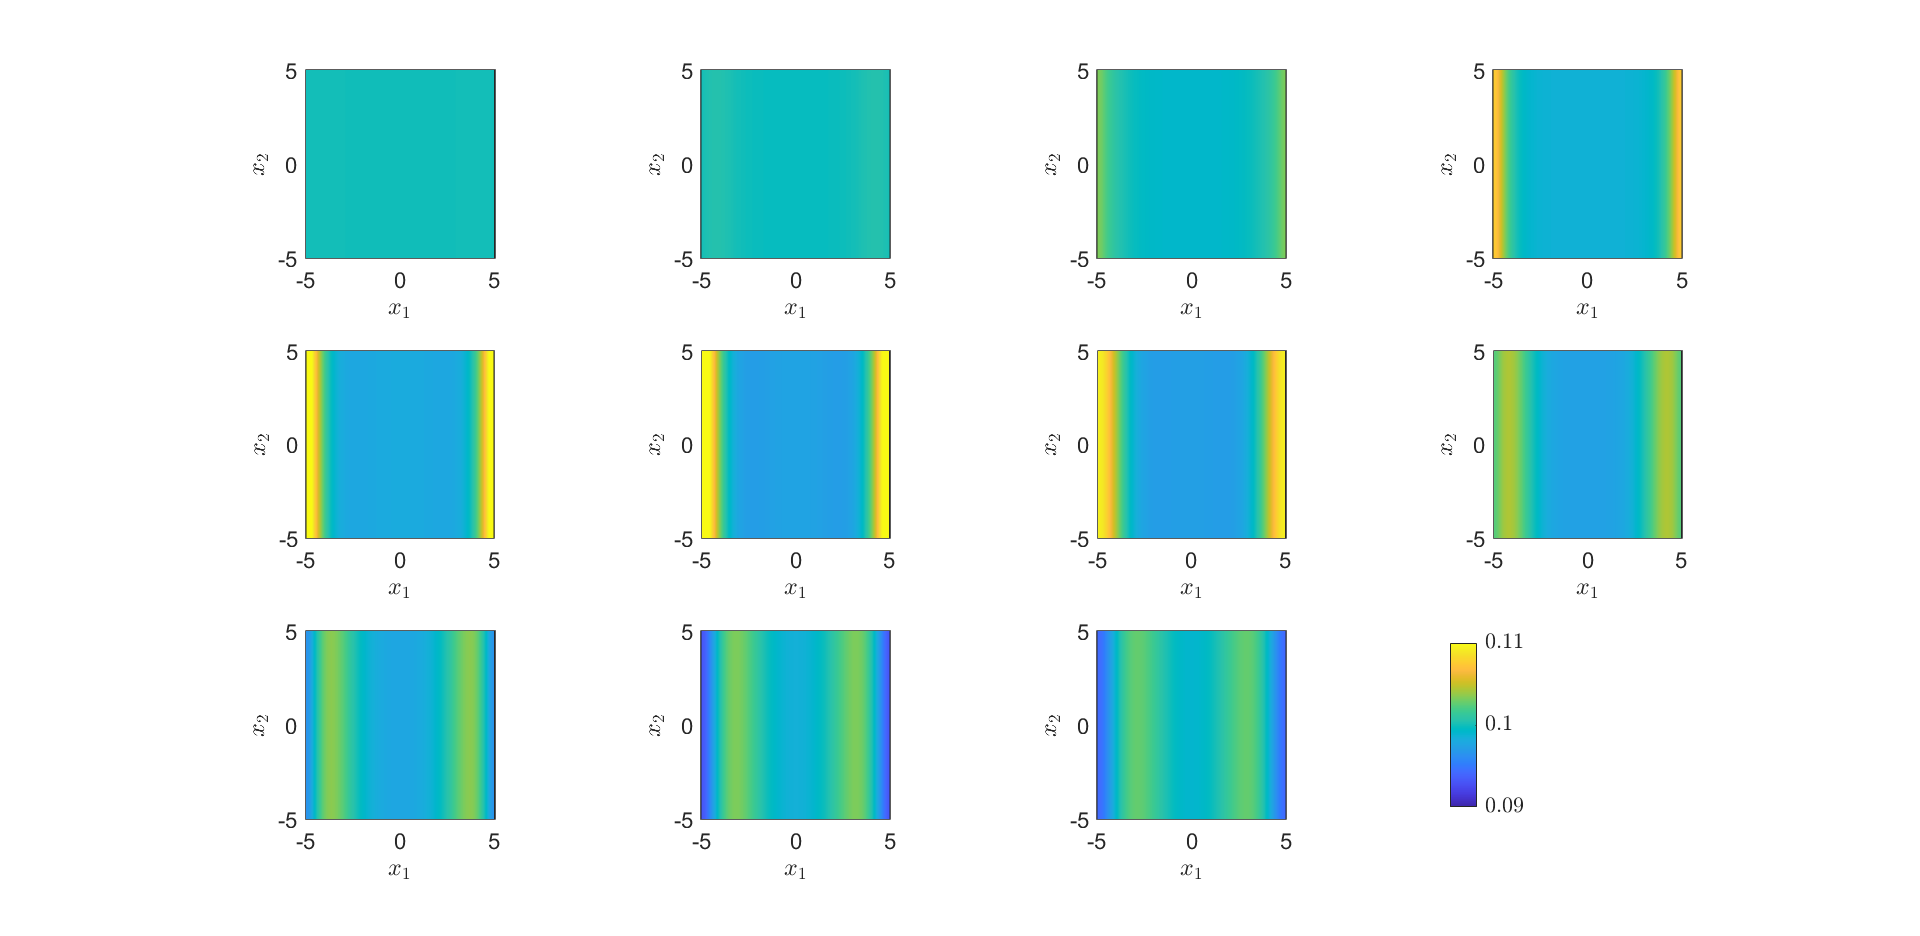
\includegraphics[scale=0.35]{rhoOptk0V.png}
	\caption{Examples Section \ref{sec:VaryExPotential}: Optimal $\rho$ over time horizon, $\kappa = 0$, $V_{ext}$ corresponding to $\hr$ in Figure \ref{F0c}} 
	\label{F3a}
\end{figure}
\begin{figure}[h]
	\centering
	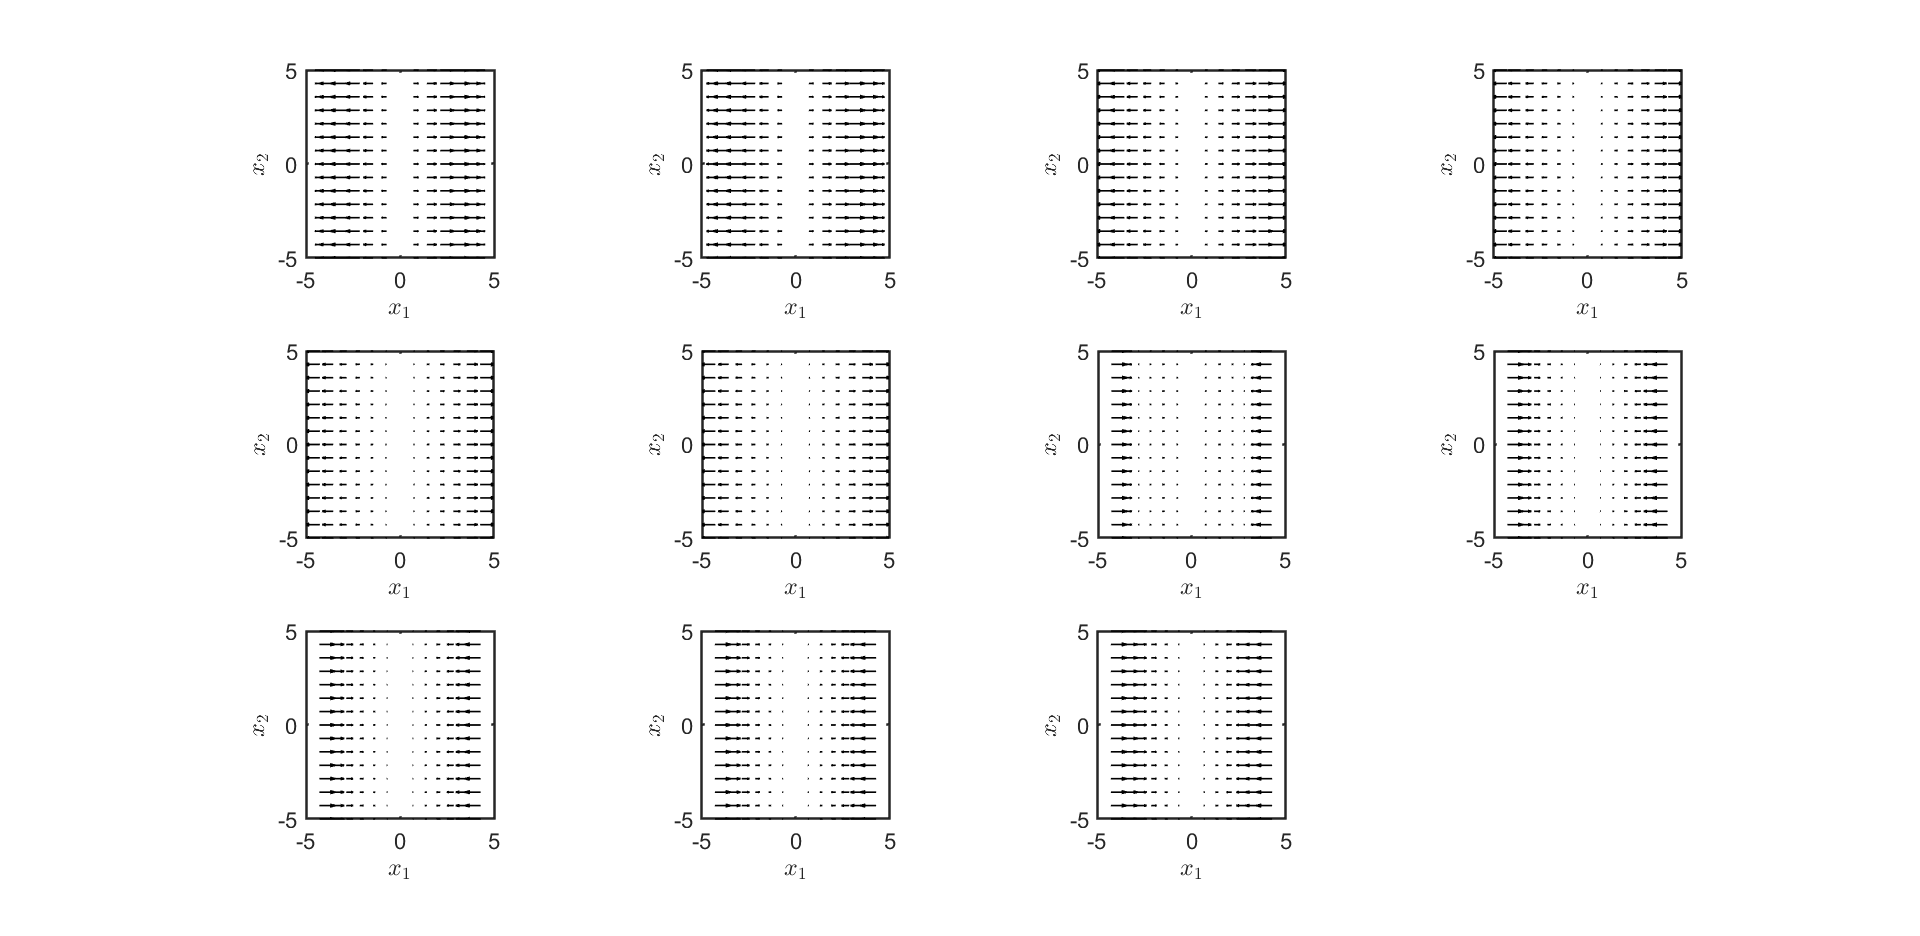
\includegraphics[scale=0.35]{ConOptk0V.png}
	\caption{Examples Section \ref{sec:VaryExPotential}: Optimal control corresponding to optimal state \ref{F3a}, $\kappa = 0$.} 
	\label{F3b}
\end{figure}

Next we set $\hr$ to be as defined in Figure \ref{F2a}. The uncontrolled state corresponds to Figure \ref{F0a}. We get that $\mathcal J_{FW} = 0.0027$ and $J_{Opt} = 0.0010$. The results can be seen in Figure \ref{F3c} and \ref{F3d}.

\begin{figure}[h]
	\centering
	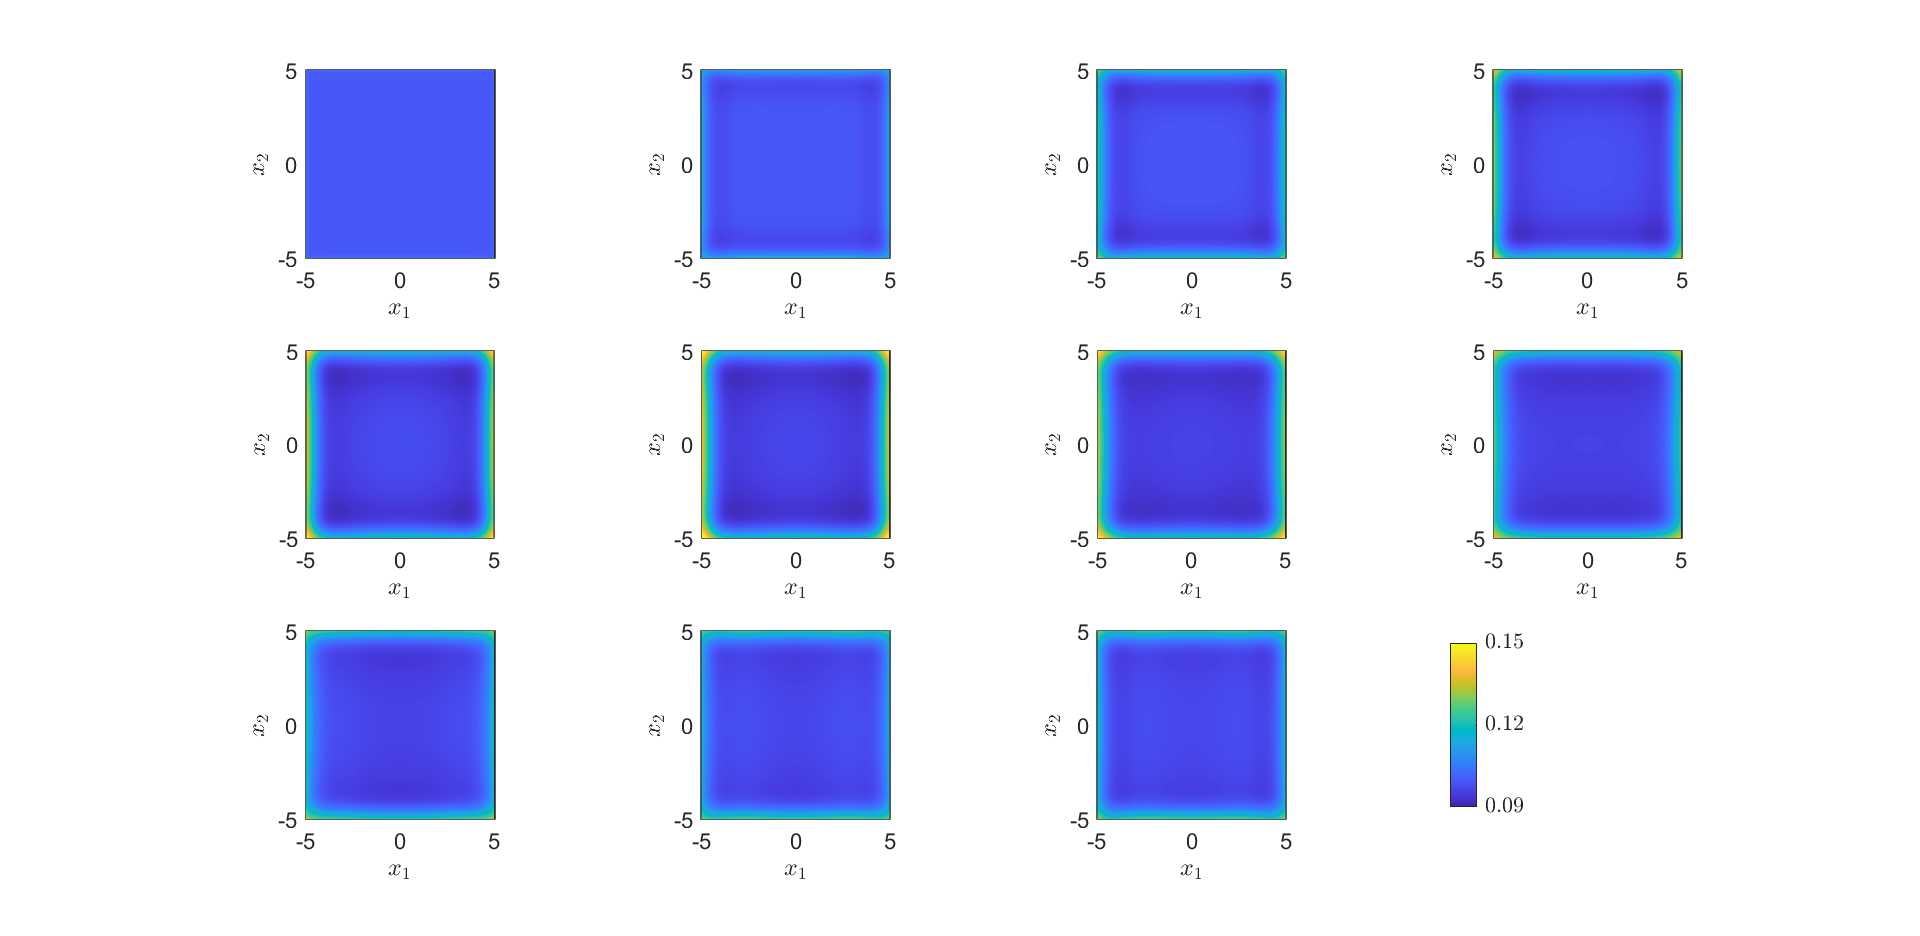
\includegraphics[scale=0.35]{rhoOptkV.png}
	\caption{Examples Section \ref{sec:VaryExPotential}: Optimal $\rho$ over time horizon, $\kappa = 2$, $V_{ext}$ corresponding to $\hr$ in Figure \ref{F2a}} 
	\label{F3c}
\end{figure}
\begin{figure}[h]
	\centering
	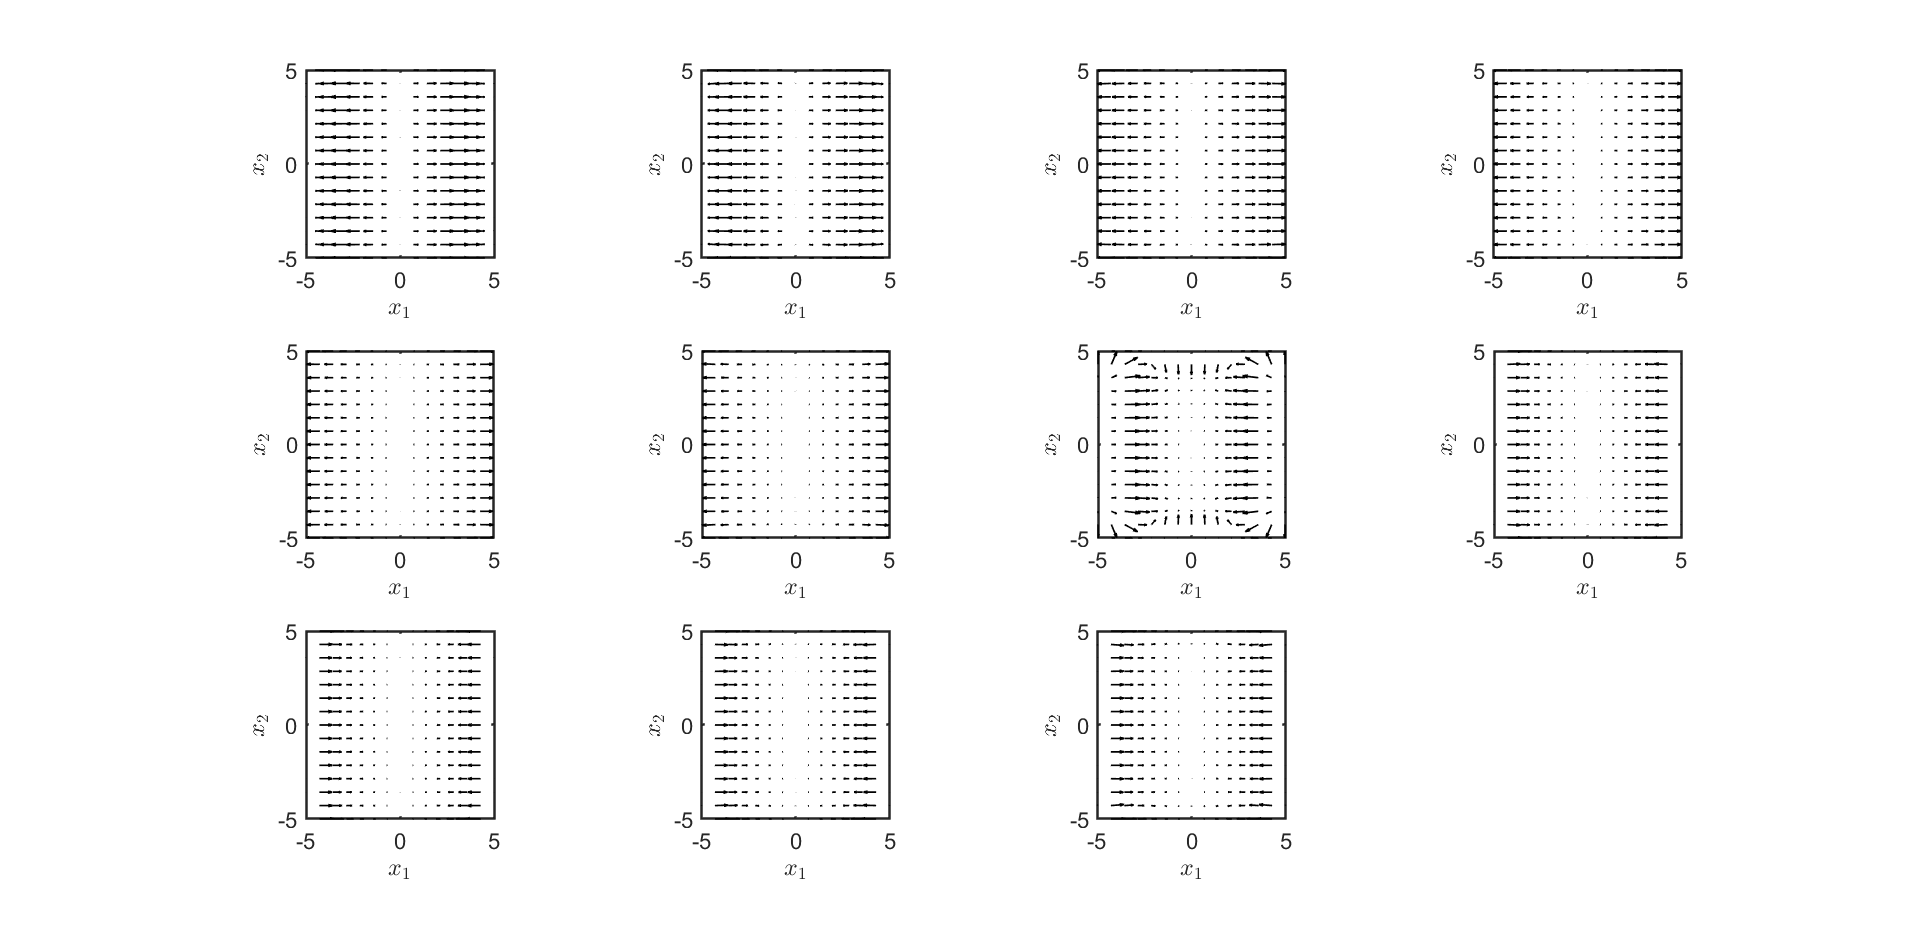
\includegraphics[scale=0.35]{ConOptkV.png}
	\caption{Examples Section \ref{sec:VaryExPotential}: Optimal control corresponding to optimal state \ref{F3c}, $\kappa = 0$.} 
	\label{F3d}
\end{figure}


Finally we set $\hr$ to be as defined in Figure \ref{F2b}. The uncontrolled state corresponds to Figure \ref{F0b}. We get that $\mathcal J_{FW} = 0.0033$ and $J_{Opt} = 0.0010$. The results can be seen in Figure \ref{F3e} and \ref{F3f}.

\begin{figure}[h]
	\centering
	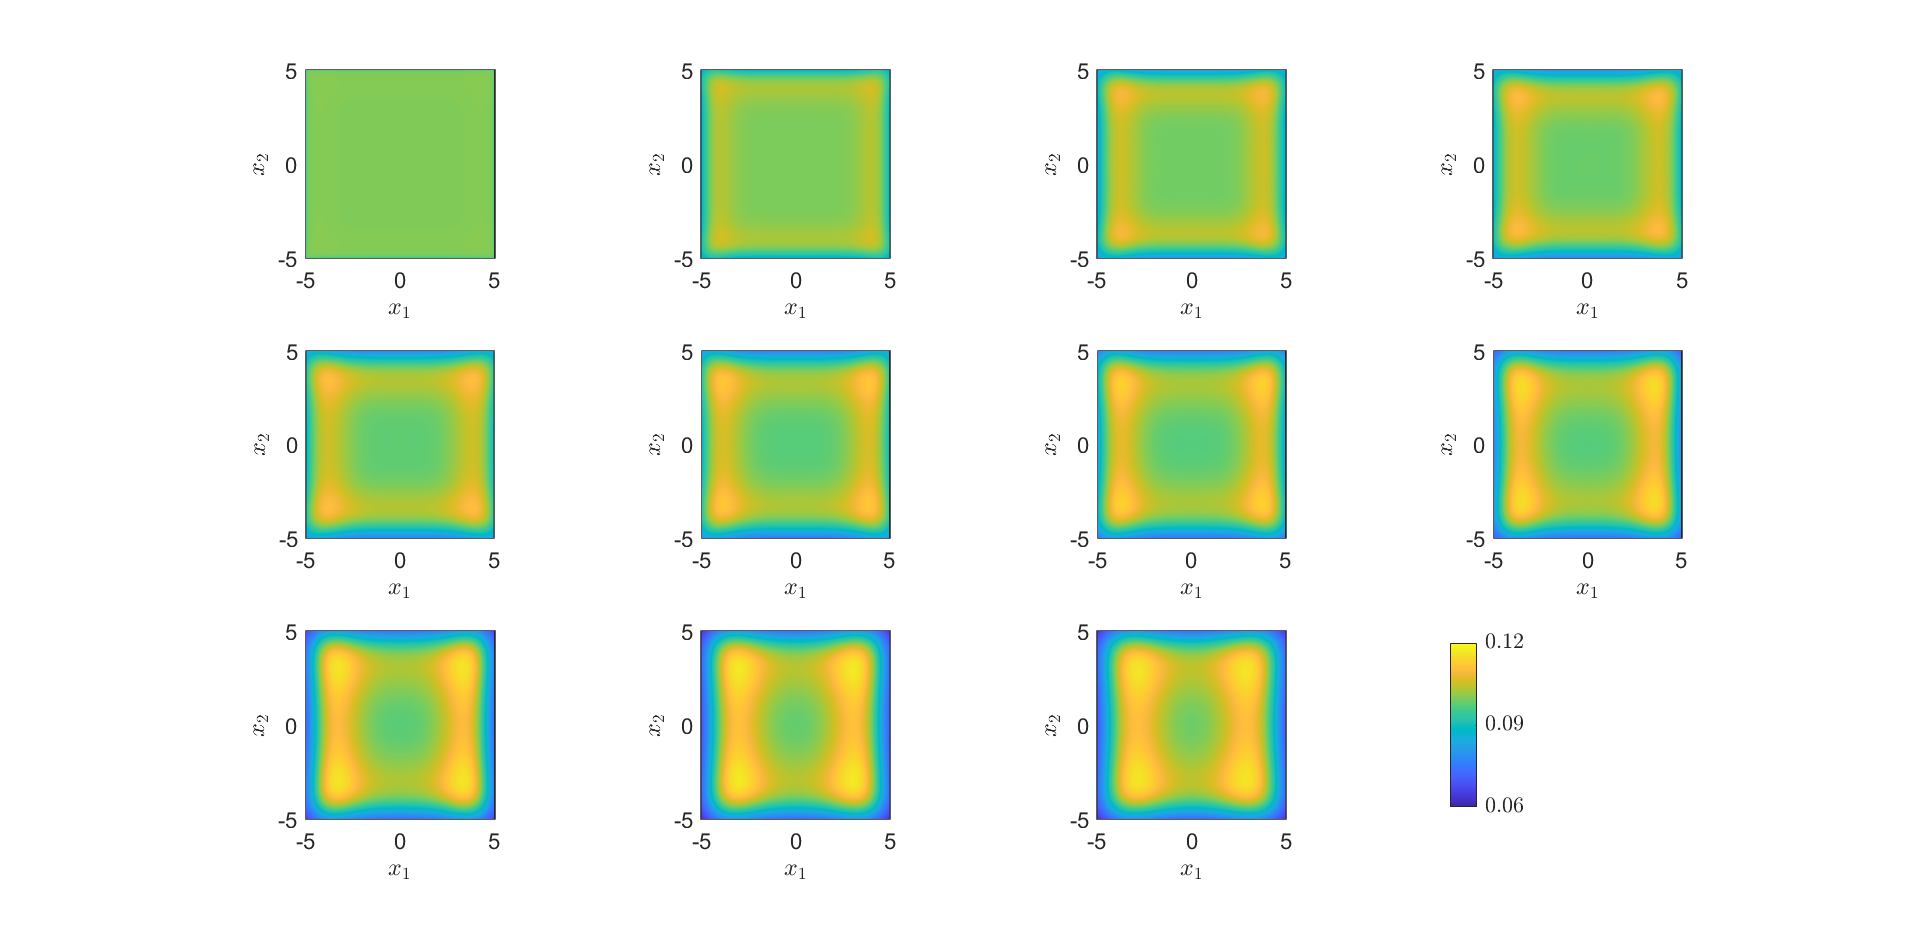
\includegraphics[scale=0.35]{rhoOptknV.png}
	\caption{Examples Section \ref{sec:VaryExPotential}: Optimal $\rho$ over time horizon, $\kappa = -2$, $V_{ext}$ corresponding to $\hr$ in Figure \ref{F2b}} 
	\label{F3e}
\end{figure}
\begin{figure}[h]
	\centering
	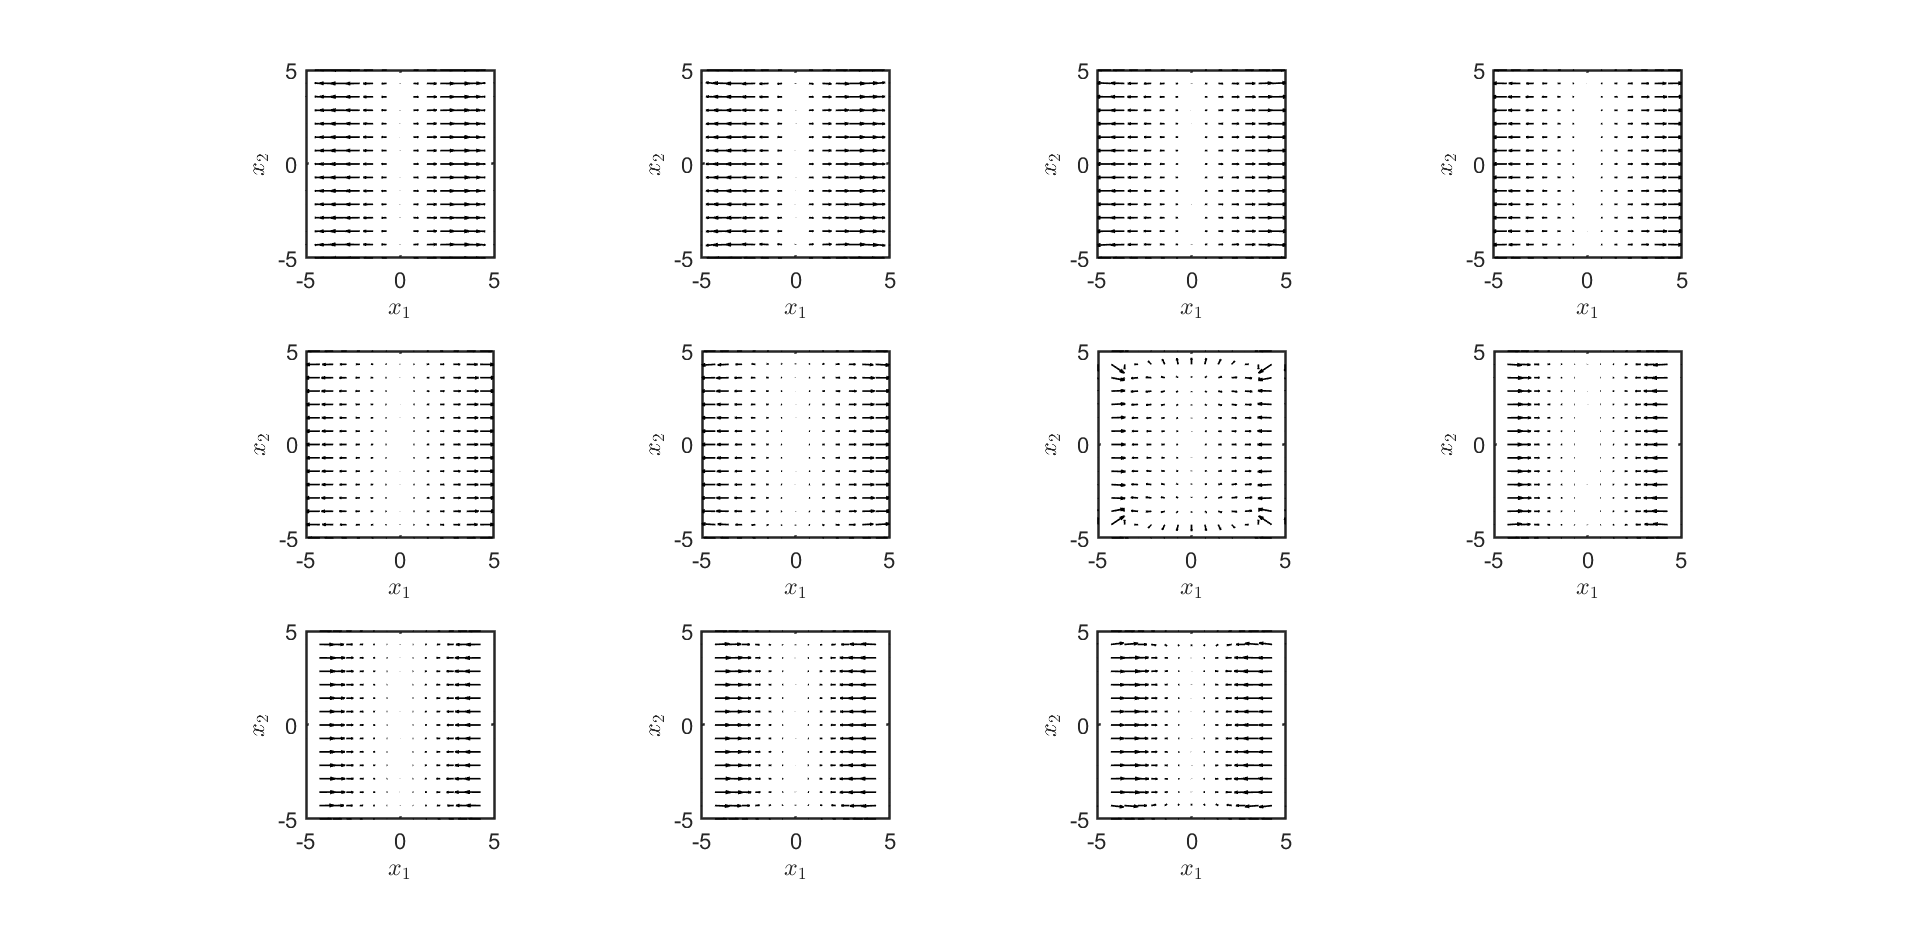
\includegraphics[scale=0.35]{ConOptknV.png}
	\caption{Examples Section \ref{sec:VaryExPotential}: Optimal control corresponding to optimal state \ref{F3e}, $\kappa = 0$.} 
	\label{F3f}
\end{figure}



\section{Periodic vs no-flux Archer}
(Note to self: a lot already in Sedimentation write up. Corresponding files u.a. SedimentationPeriodicOCP
SedimentationNoFluxOCP)\\
\\
We now move to another DDFT, which takes volume exclusion into account. This follows the Archer paper on sedimentation. We also have a different pair potential in this case.
\subsection{Comparing Periodic and No-Flux Targets} \label{sec:PeriodicNoFlux1}
(Note: PeriodicvsNoFluxOCP in code)
We are interested in the effect of giving a periodic target to a no-flux dynamics problem and of giving a target created from no-flux dynamics to a periodic optimal control problem. We define the spatial domain to be $[0,10]^2$, with $N = 30$ and the time horizon is $(0,3)$ with $n = 30$. The ODE tolerances are $10^{-8}$ and optimality tolerances are $10^{-}$. We set $\lambda = 0.01$ and $\beta = 10^{-3}$. The interaction strength is $\kappa  = -2$.

At first we set the periodic target to be a forward problem solved on a periodic box, influenced by an external potential modelling gravity of strength $0.1$ and by a pair potential of strength $\kappa = -2$, see Figure \ref{F4}. The initial condition for $\rho$ is a uniform distribution $\rho_0 = 0.08$. 
This target is interpolated onto the points of a box with no-flux boundary conditions. The optimal control problem is solved on a box. The dynamics are also influenced by the external and pair potential, and the initial condition for $\rho$ is the same as for the target. The only difference in the setup is whether we solve the problem on a periodic box or on a box with no-flux boundary conditions. This uncontrolled state is the dynamics displayed in Figure \ref{F4c}. The optimal state and control can be seen in figures \ref{F4a} and \ref{F4b}. The cost functionals are $\mathcal J_{FW} = 0.0043$ and $\mathcal J_{Opt} = 0.0012$.

\begin{figure}[h]
	\centering
	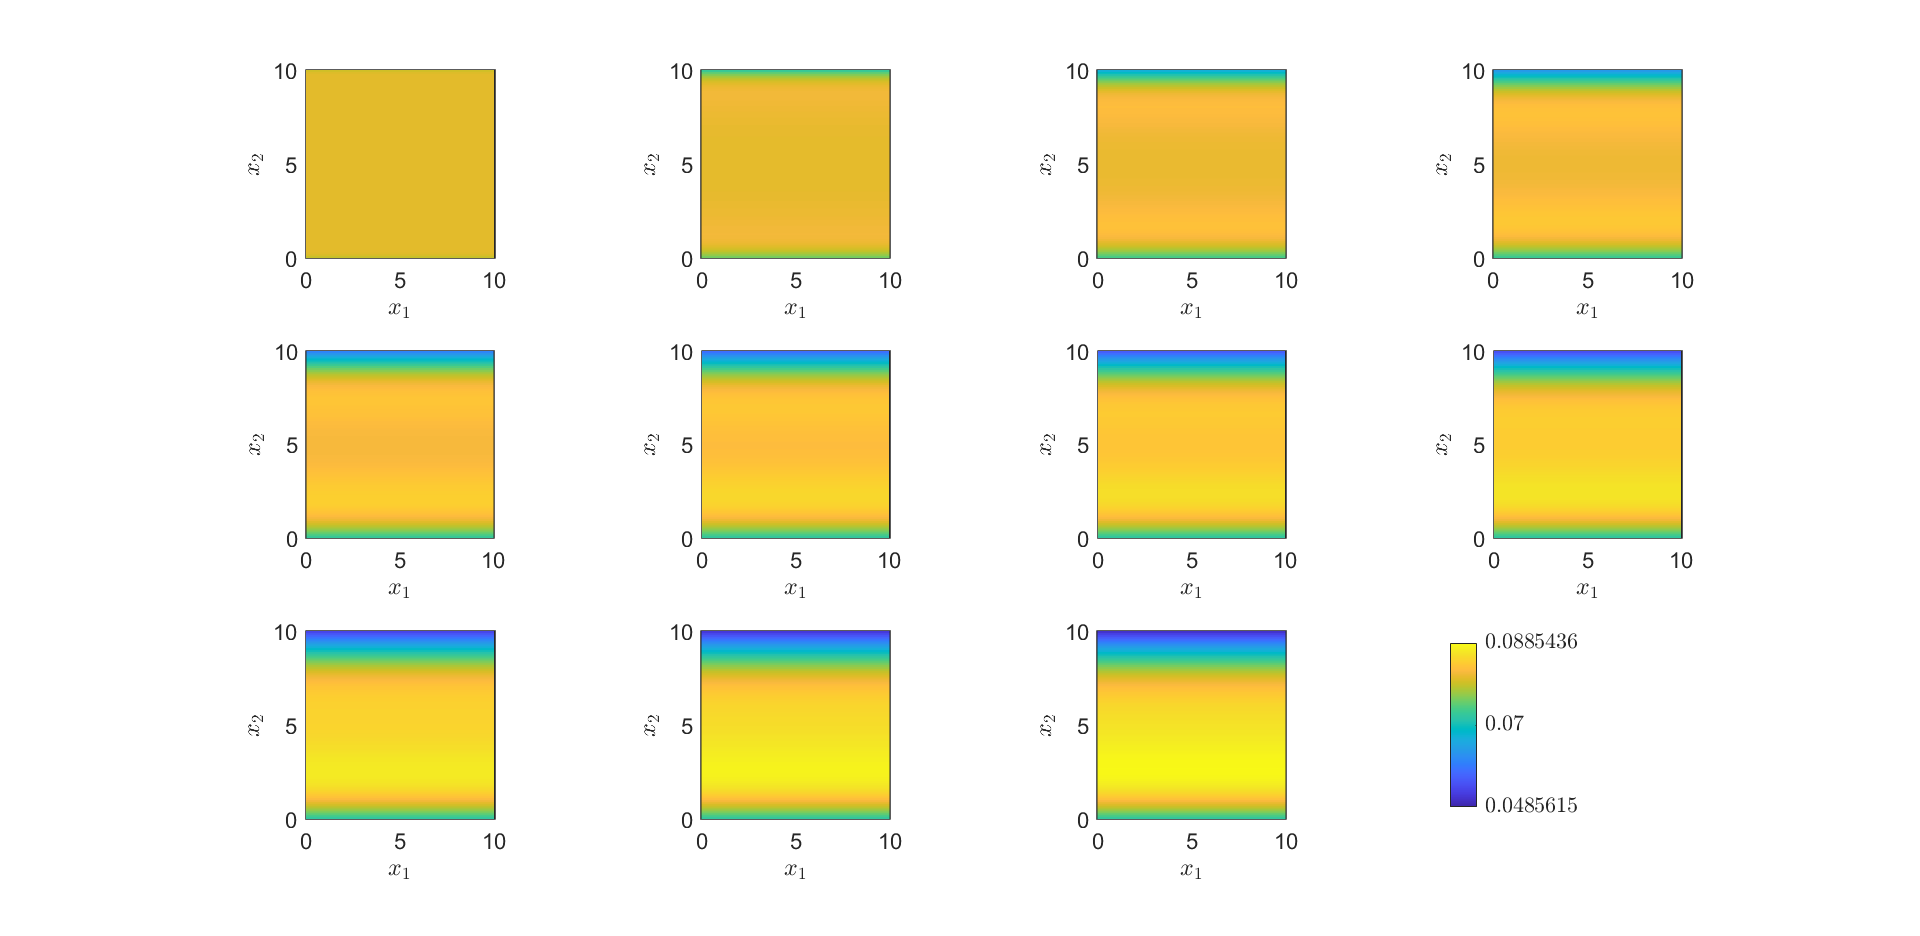
\includegraphics[scale=0.35]{rhoHatPeri1.png}
	\caption{Examples Section \ref{sec:PeriodicNoFlux1}: $\hr$ created in a periodic box corresponding to optimal state in Figure \ref{F4a}.} 
	\label{F4}
\end{figure}
\begin{figure}[h]
	\centering
	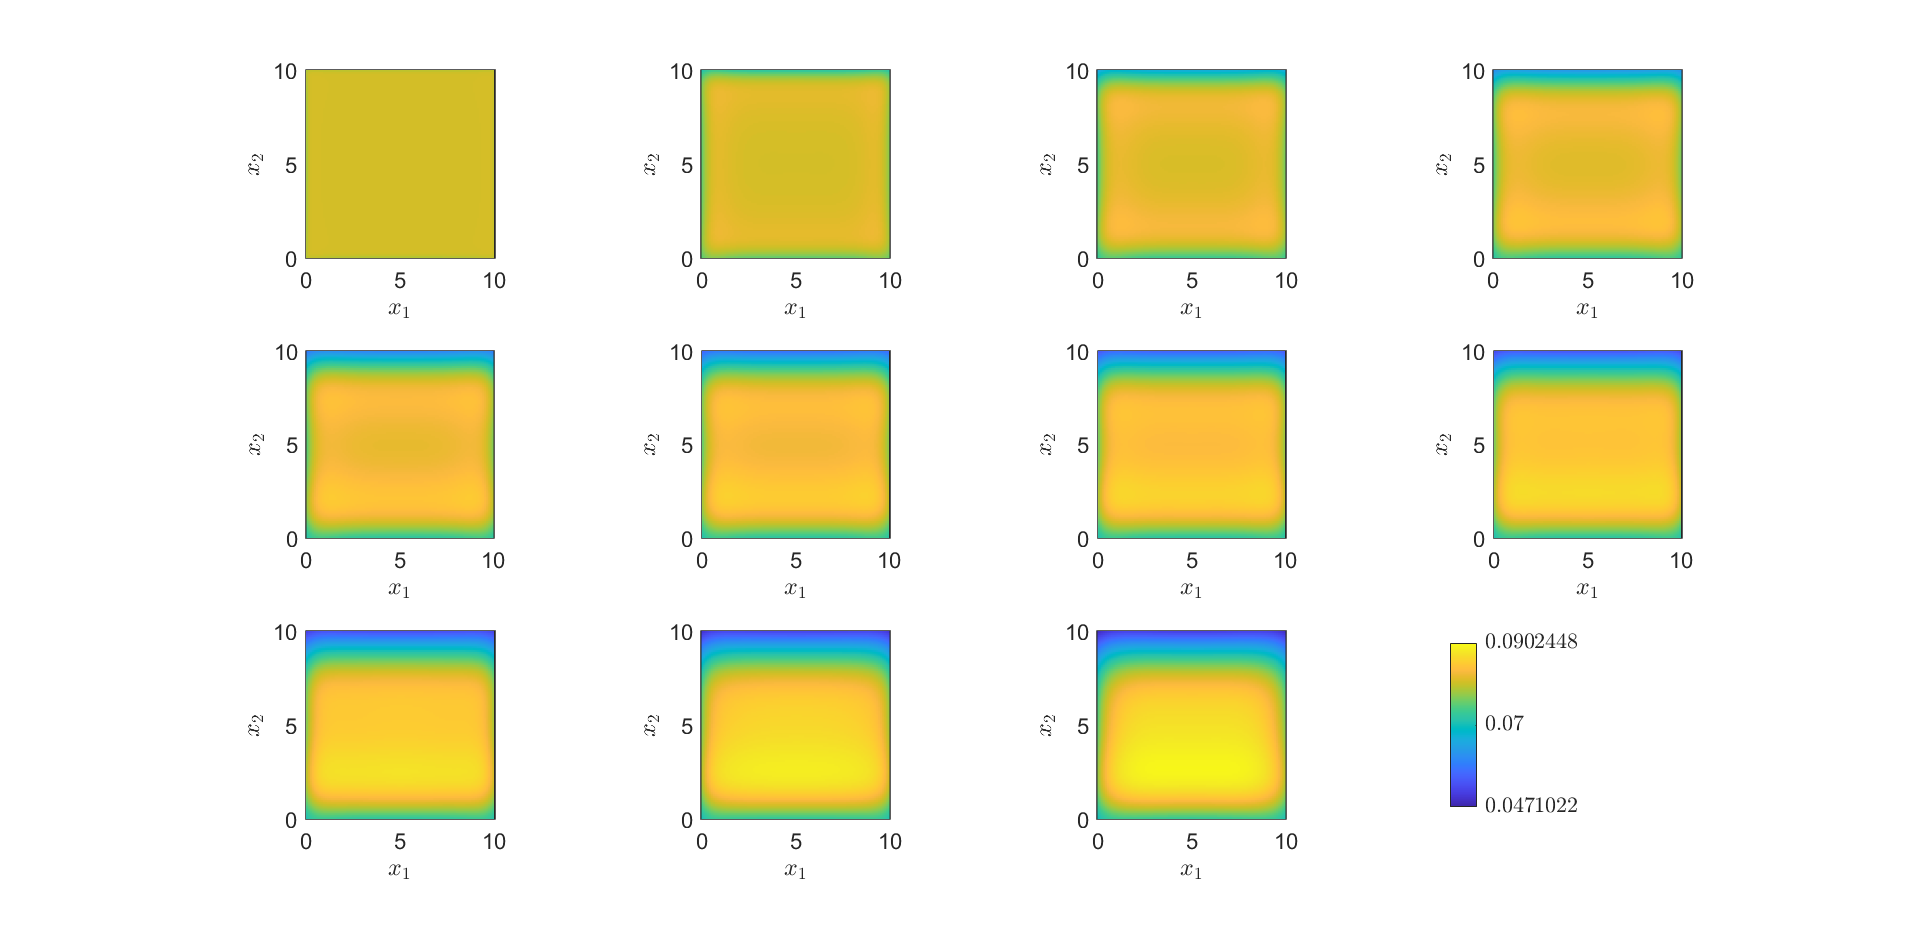
\includegraphics[scale=0.35]{rhoOptPeri1.png}
	\caption{Examples Section \ref{sec:PeriodicNoFlux1}: Optimal state $\rho$ in no-flux box} 
	\label{F4a}
\end{figure}

\begin{figure}[h]
	\centering
	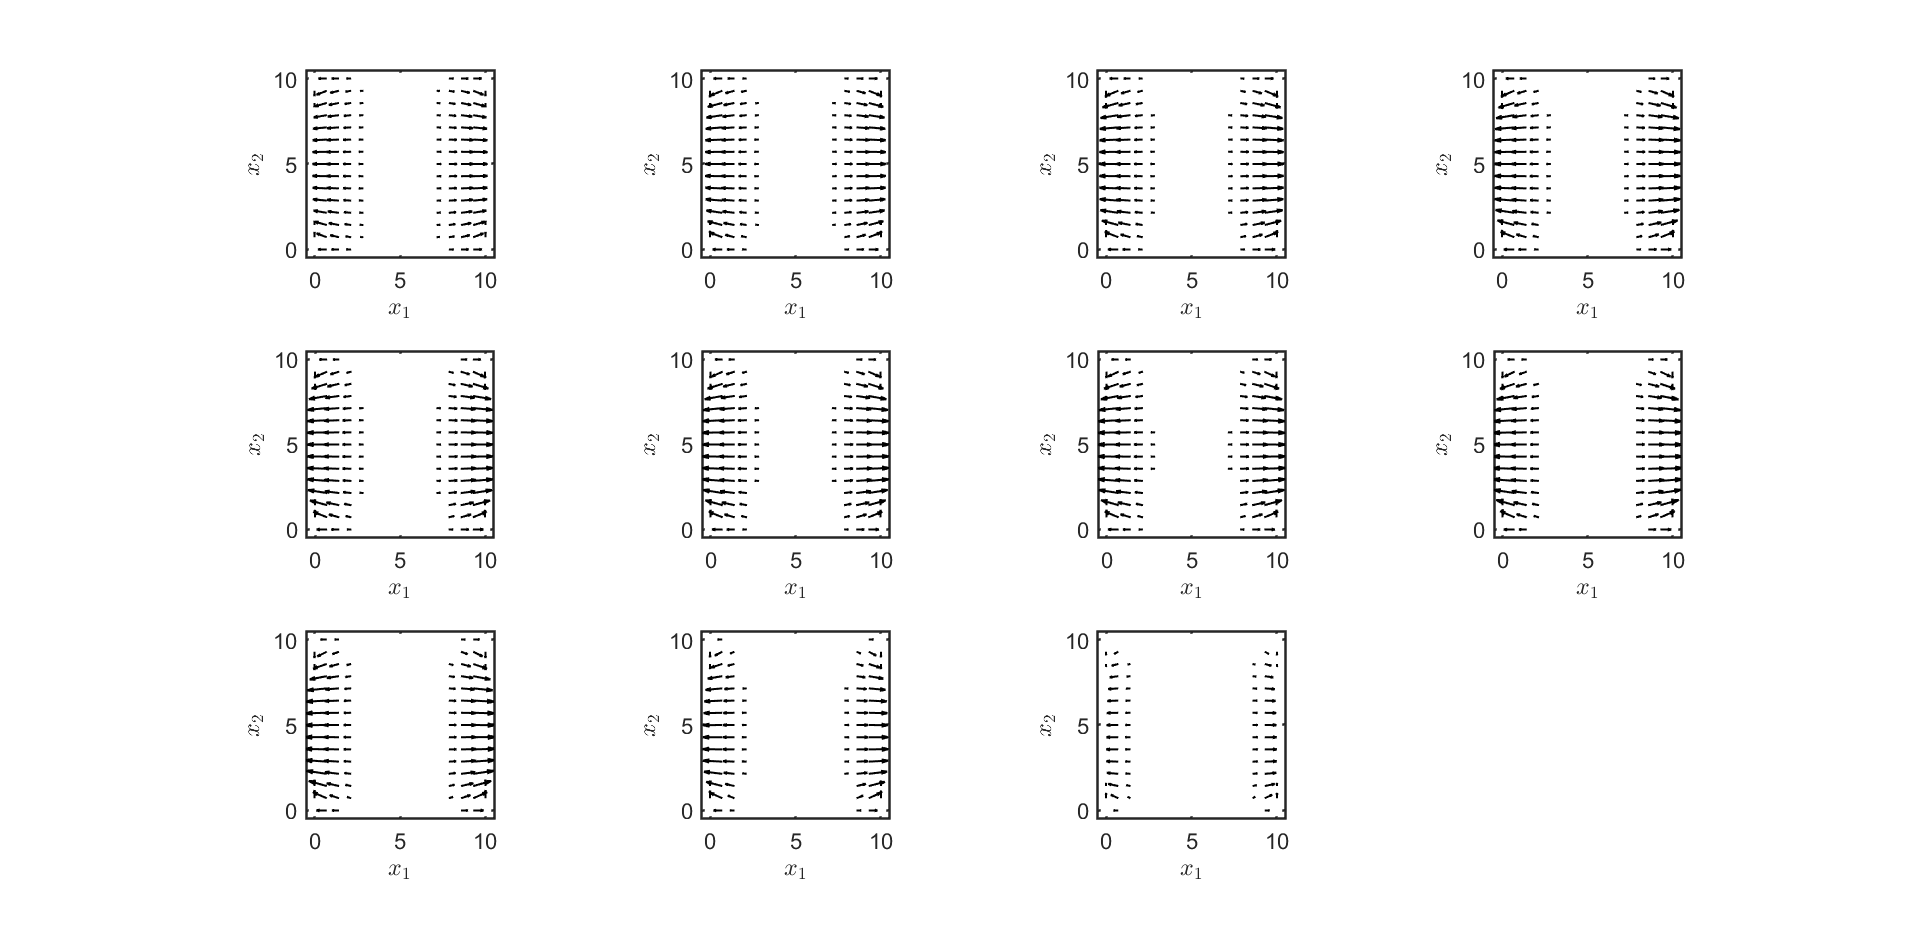
\includegraphics[scale=0.35]{ConOptPeri1.png}
	\caption{Examples Section \ref{sec:PeriodicNoFlux1}: Optimal control corresponding to optimal state in Figure \ref{F4a}.} 
	\label{F4b}
\end{figure}

For a second example, we do the exact opposite by setting $\hr$ to be the forward problem in a no-flux box with the same parameter choices from above, see Figure \ref{F4c}. We then compute the optimal control problem corresponding to this target on a periodic box. Note that the uncontrolled periodic solution is equivalent to the dynamics in Figure \ref{F4}. The optimal control and state are displayed in Figures \ref{F4d} and \ref{F4e}. We get $\mathcal J_{FW} =  0.0044$ and $\mathcal J_{Opt} = 0.0011$. When comparing to the values of the previous setup, we can see that the above scenario is slightly more costly than this one.

\begin{figure}[h]
	\centering
	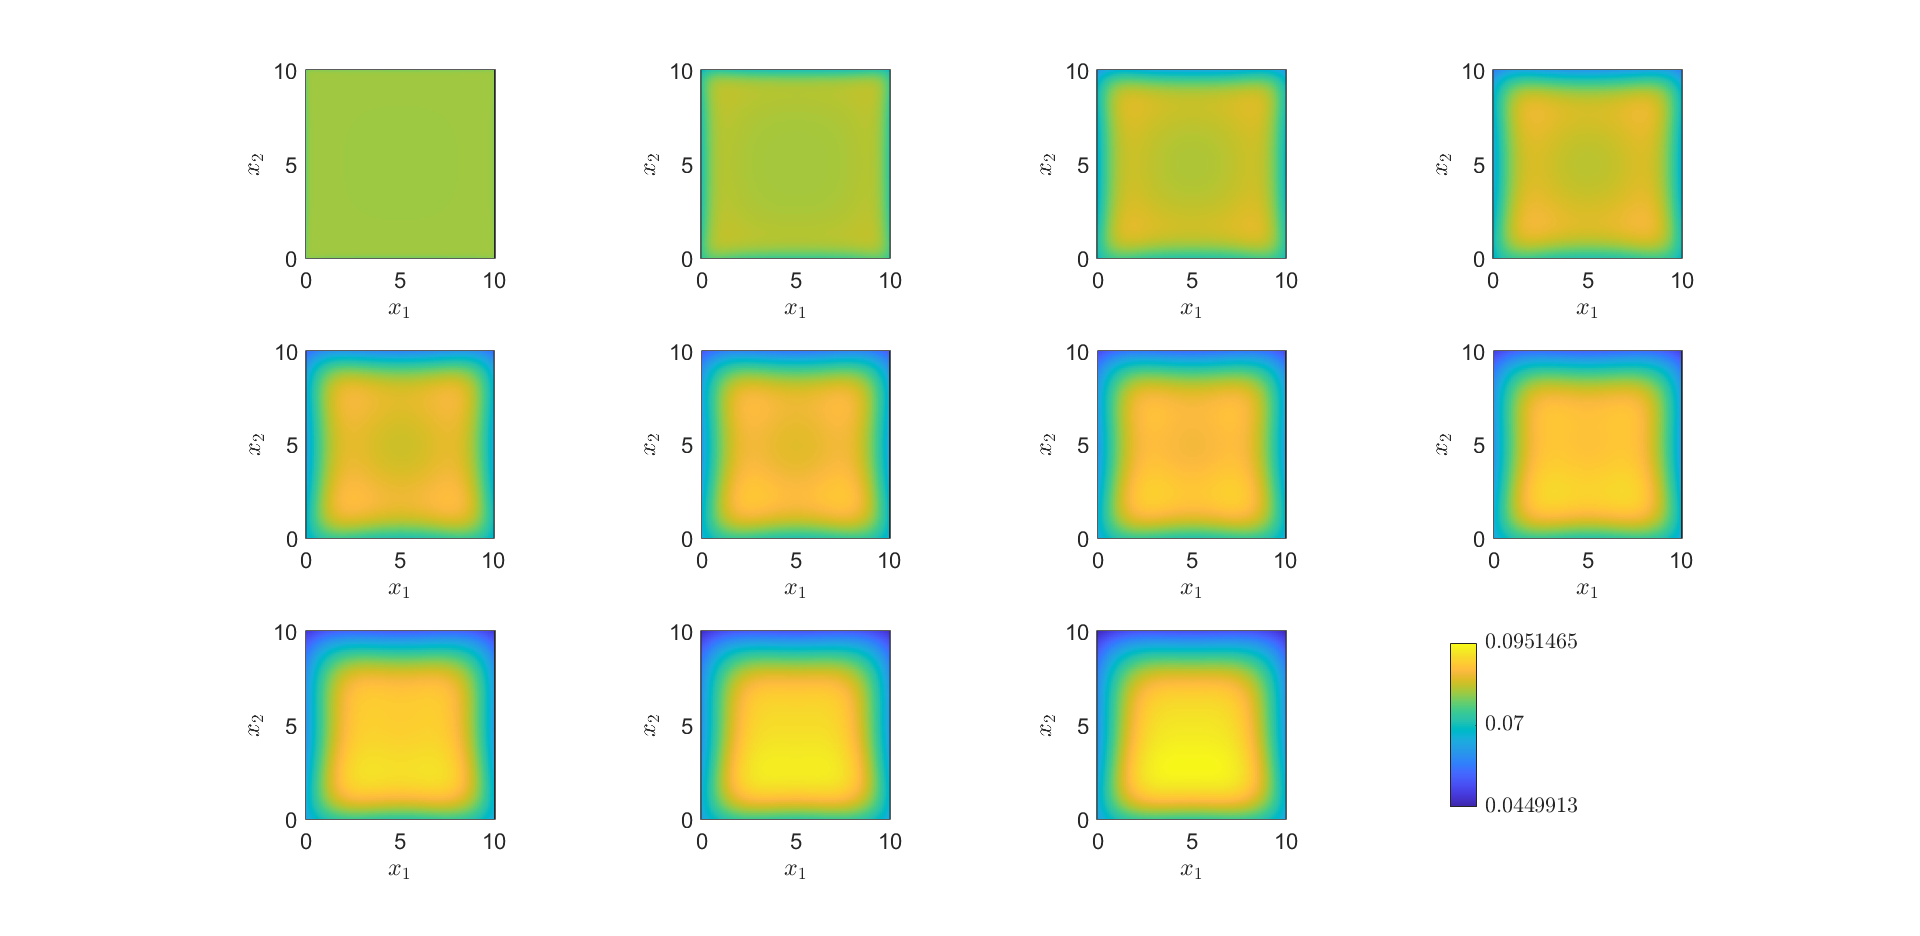
\includegraphics[scale=0.35]{rhoHatPeri2.png}
	\caption{Examples Section \ref{sec:PeriodicNoFlux1}: $\hr$ created in a no-flux box corresponding to optimal state in Figure \ref{F4d}.} 
	\label{F4c}
\end{figure}
\begin{figure}[h]
	\centering
	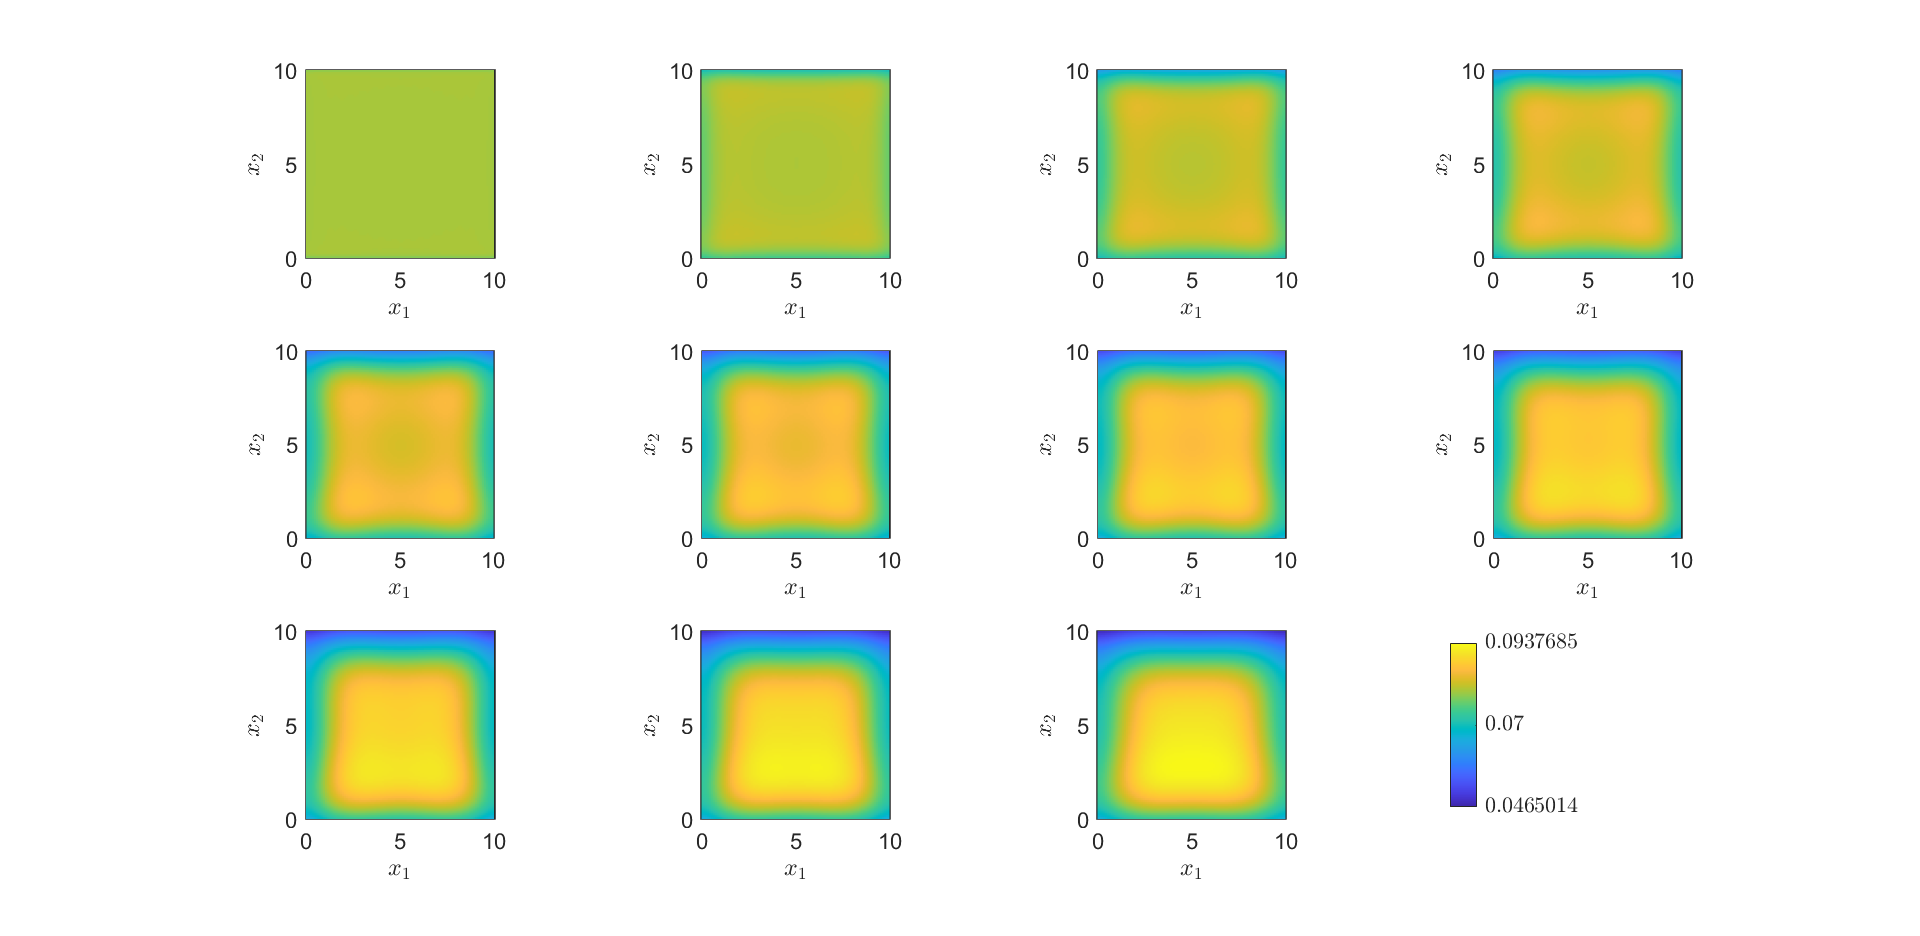
\includegraphics[scale=0.35]{rhoOptPeri2.png}
	\caption{Examples Section \ref{sec:PeriodicNoFlux1}: Optimal state $\rho$ in periodic box} 
	\label{F4d}
\end{figure}

\begin{figure}[h]
	\centering
	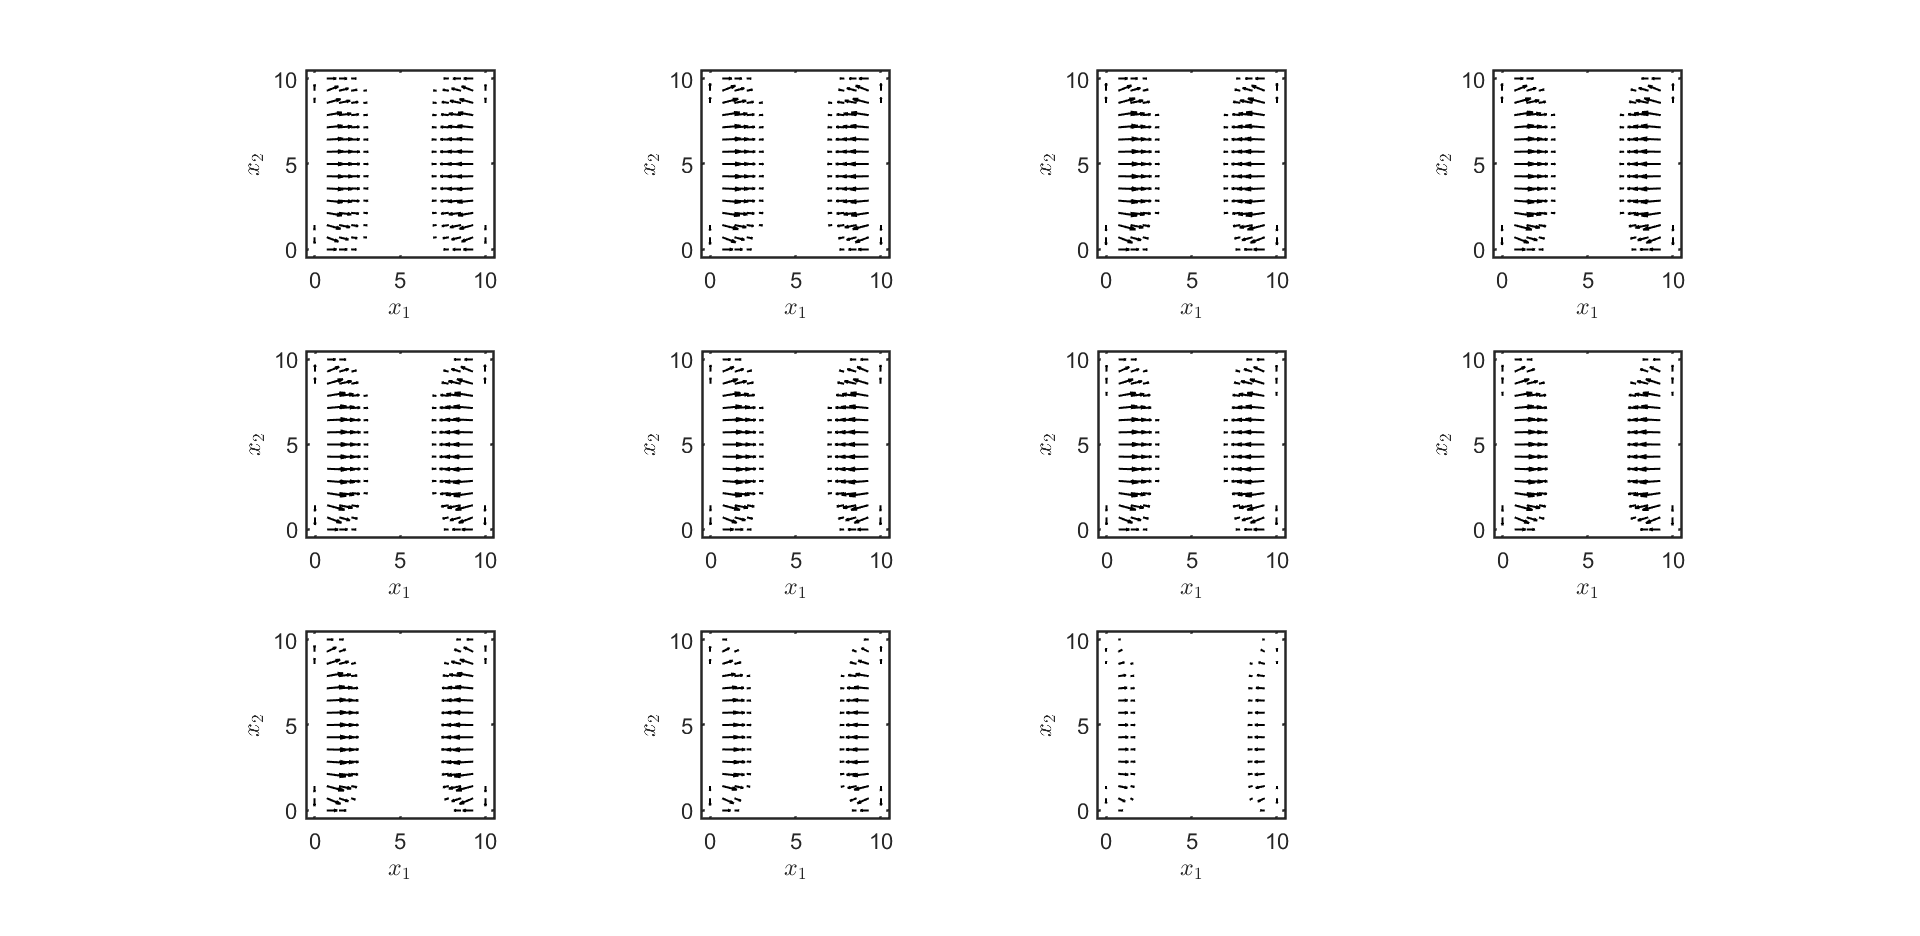
\includegraphics[scale=0.35]{ConOptPeri2.png}
	\caption{Examples Section \ref{sec:PeriodicNoFlux1}: Optimal control corresponding to optimal state in Figure \ref{F4d}.} 
	\label{F4e}
\end{figure}

In order to be able to make a direct comparison between the two scenarios, we define a target, which satisfies both periodic and no-flux conditions. This is a forward problem influenced by the same forces as above, with an initial condition
\begin{align}\label{eq:Target1}
	\hr_0 = 0.08\frac{1}{4}(\cos(0.4\pi y_2) + 4),
\end{align}
see Figure \ref{F4f}.
We then compute the optimal control problem on the no-flux box to get $\mathcal J_{FW} = 0.0087$ and $\mathcal J_{Opt} = 0.0036$. The results can be seen in Figures \ref{F4g} and \ref{F4h}.
We then compute the optimal control problem on the periodic box to get $\mathcal J_{FW} = 0.0030$ and $\mathcal J_{Opt} = 0.0019$. The results can be seen in Figures \ref{F4i} and \ref{F4j}. We can see that the periodic solution was already much closer to the target in the beginning and therefore the final cost was much lower. In this case, the periodicity of the solution impacted the cost positively. However, this also shows that the cost of a real life no-flux problem may be higher than anticipated when running a periodic problem to approximate a no-flux situation.
\begin{figure}[h]
	\centering
	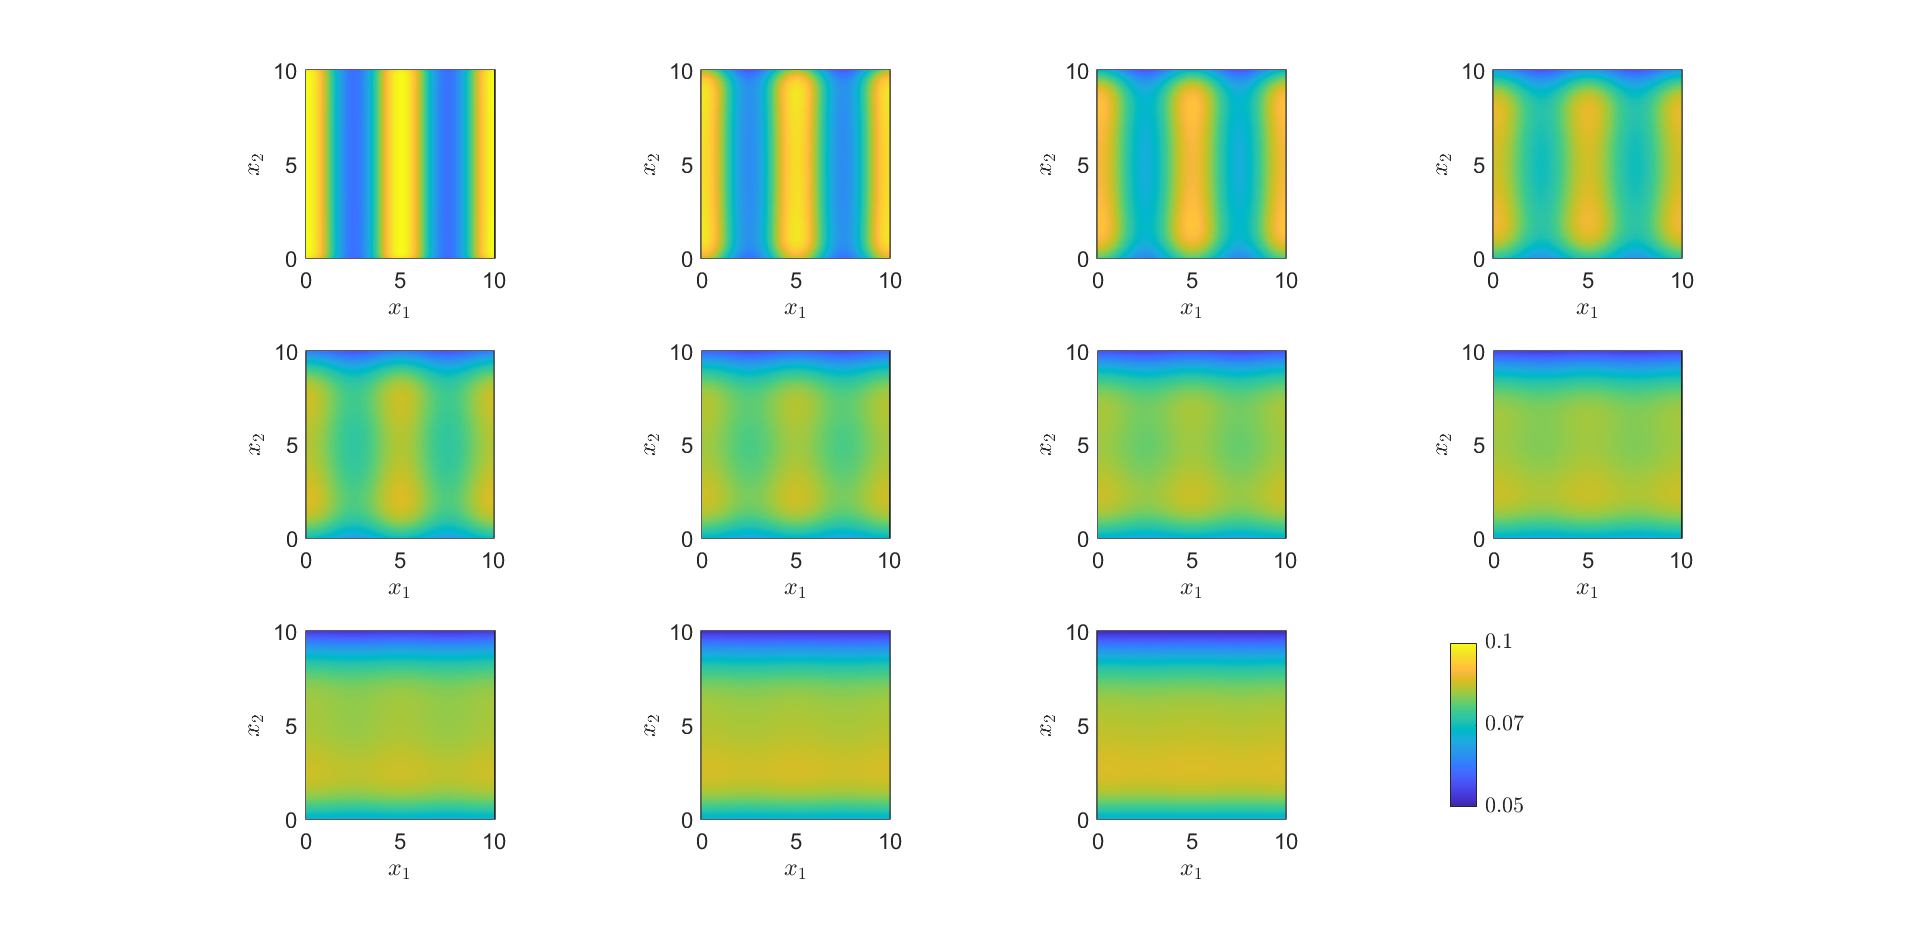
\includegraphics[scale=0.35]{rhoHatPeri3.png}
	\caption{Examples Section \ref{sec:PeriodicNoFlux1}: $\hr$ from equation \ref{eq:Target1} corresponding to optimal state in Figure \ref{F4g}.} 
	\label{F4f}
\end{figure}
\begin{figure}[h]
	\centering
	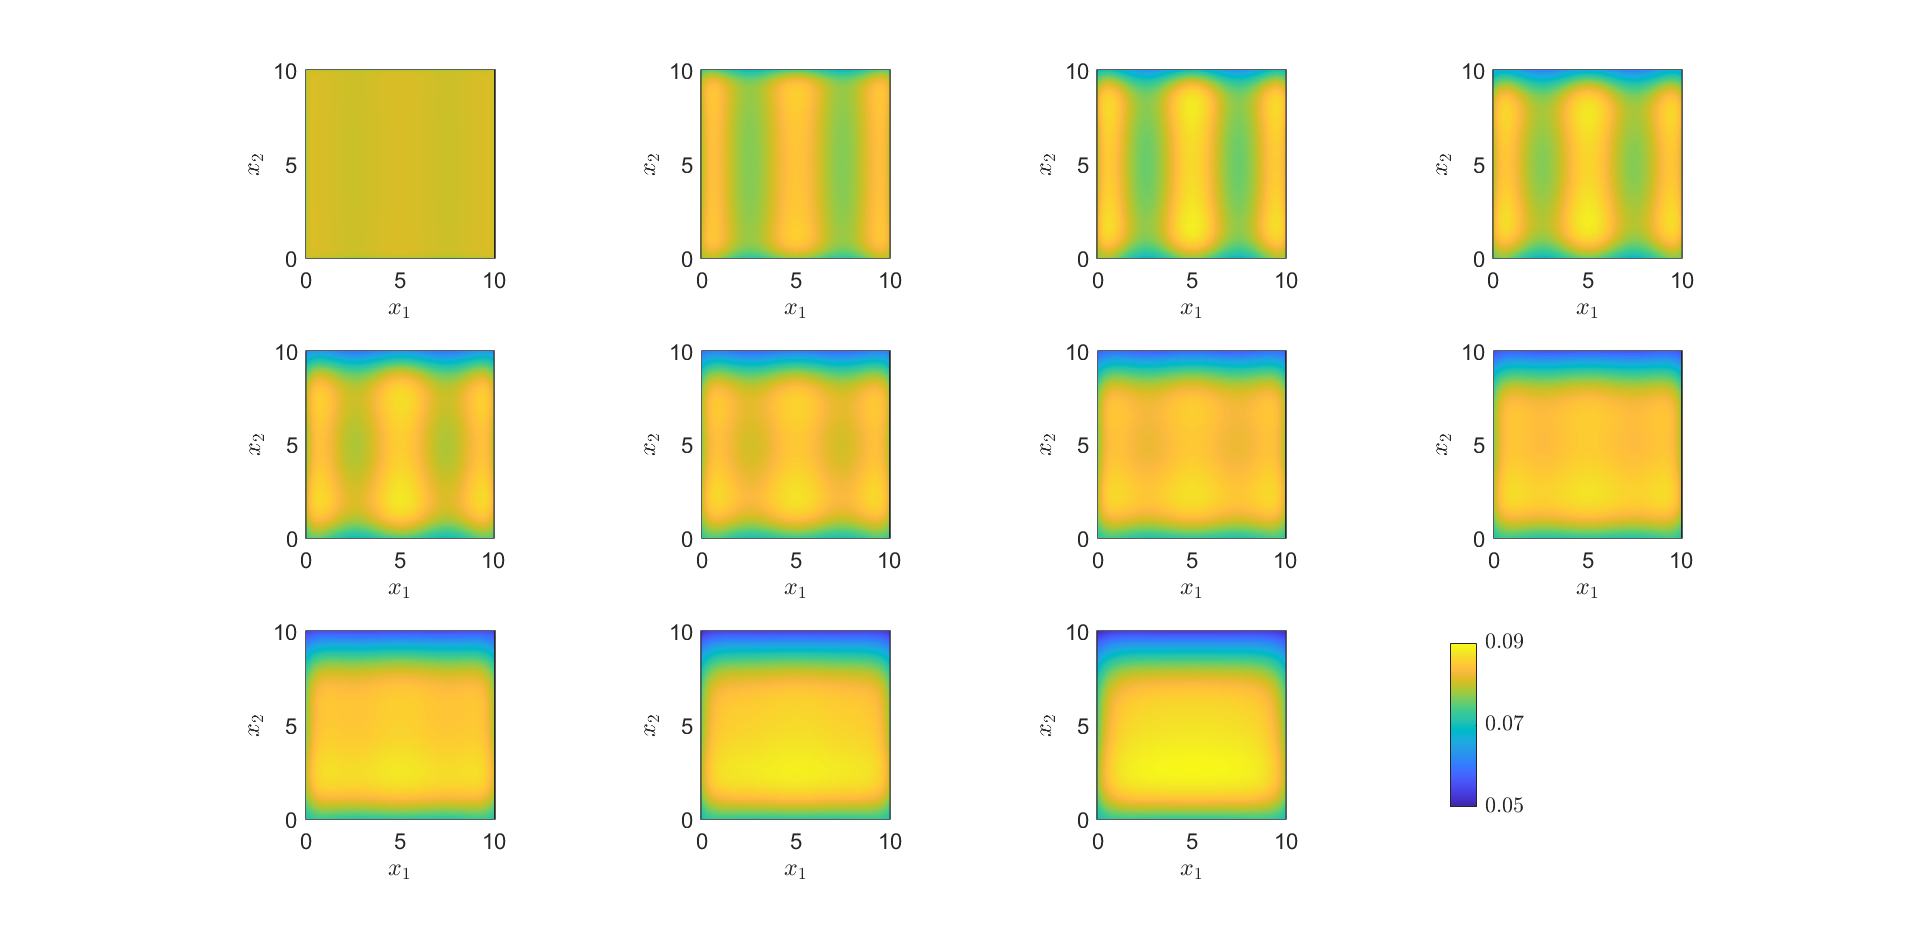
\includegraphics[scale=0.35]{rhoOptPeri3.png}
	\caption{Examples Section \ref{sec:PeriodicNoFlux1}: Optimal state $\rho$ in no-flux box} 
	\label{F4g}
\end{figure}

\begin{figure}[h]
	\centering
	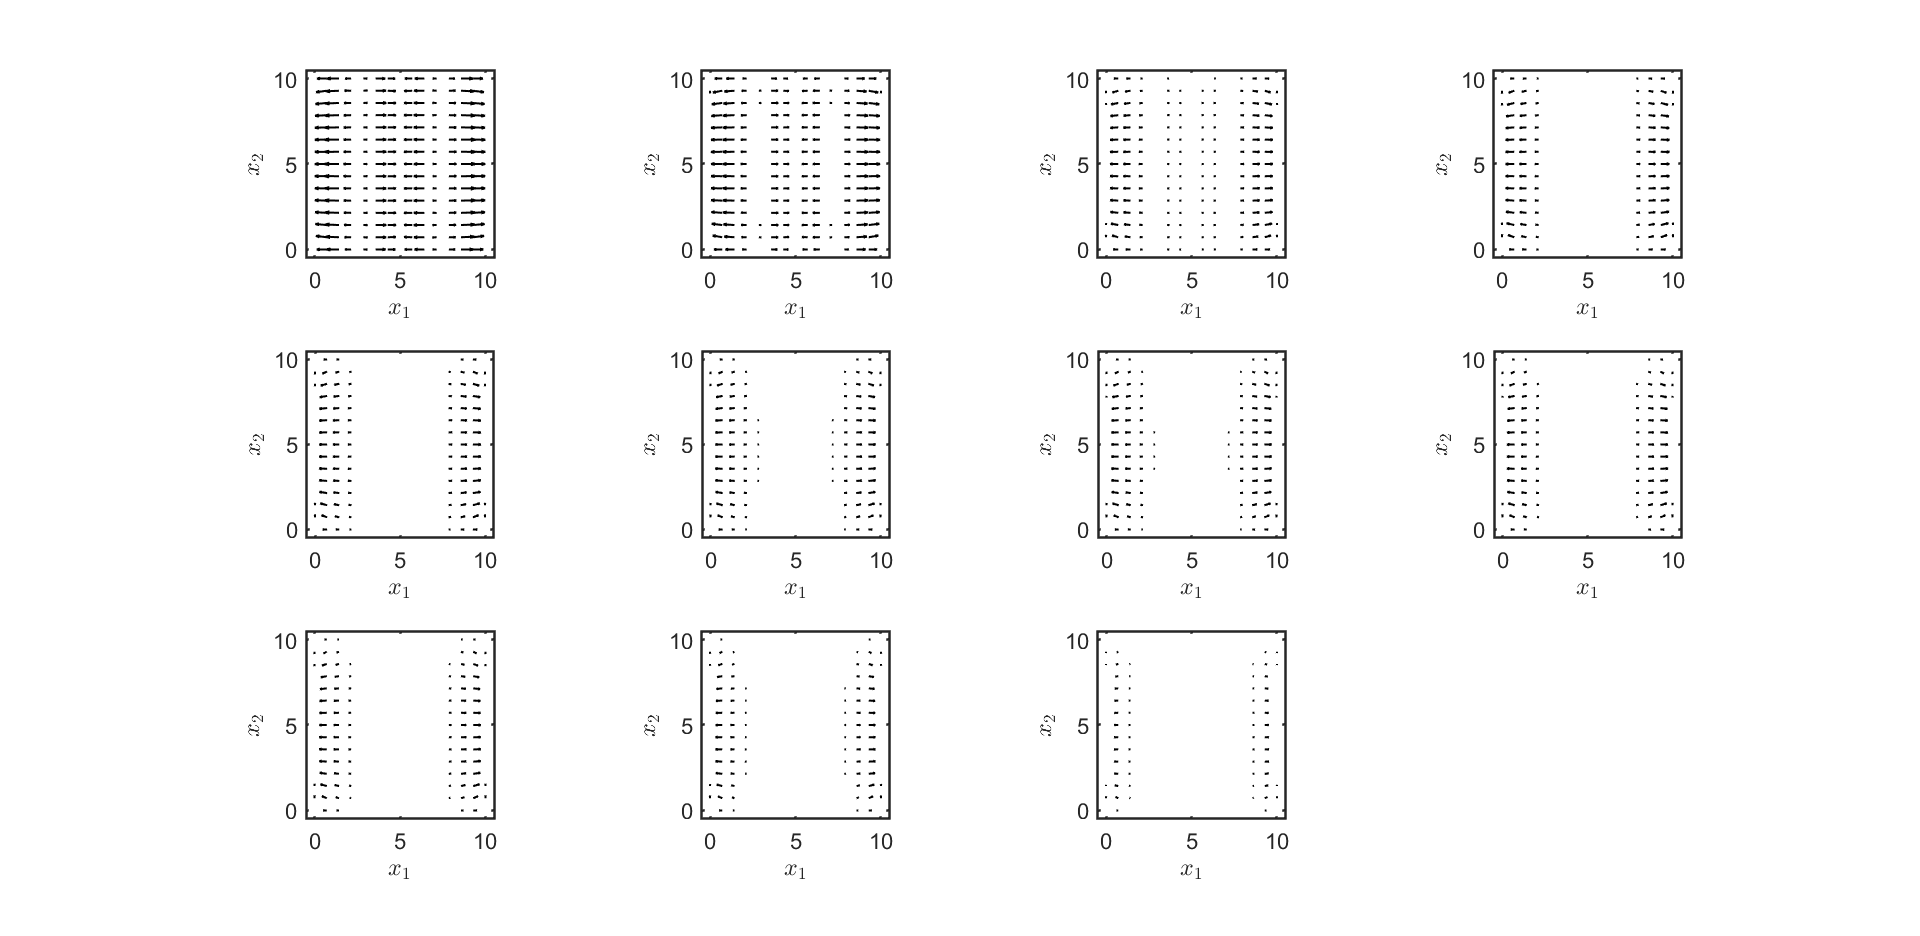
\includegraphics[scale=0.35]{ConOptPeri3.png}
	\caption{Examples Section \ref{sec:PeriodicNoFlux1}: Optimal control corresponding to optimal state in Figure \ref{F4g}.} 
	\label{F4h}
\end{figure}

\begin{figure}[h]
	\centering
	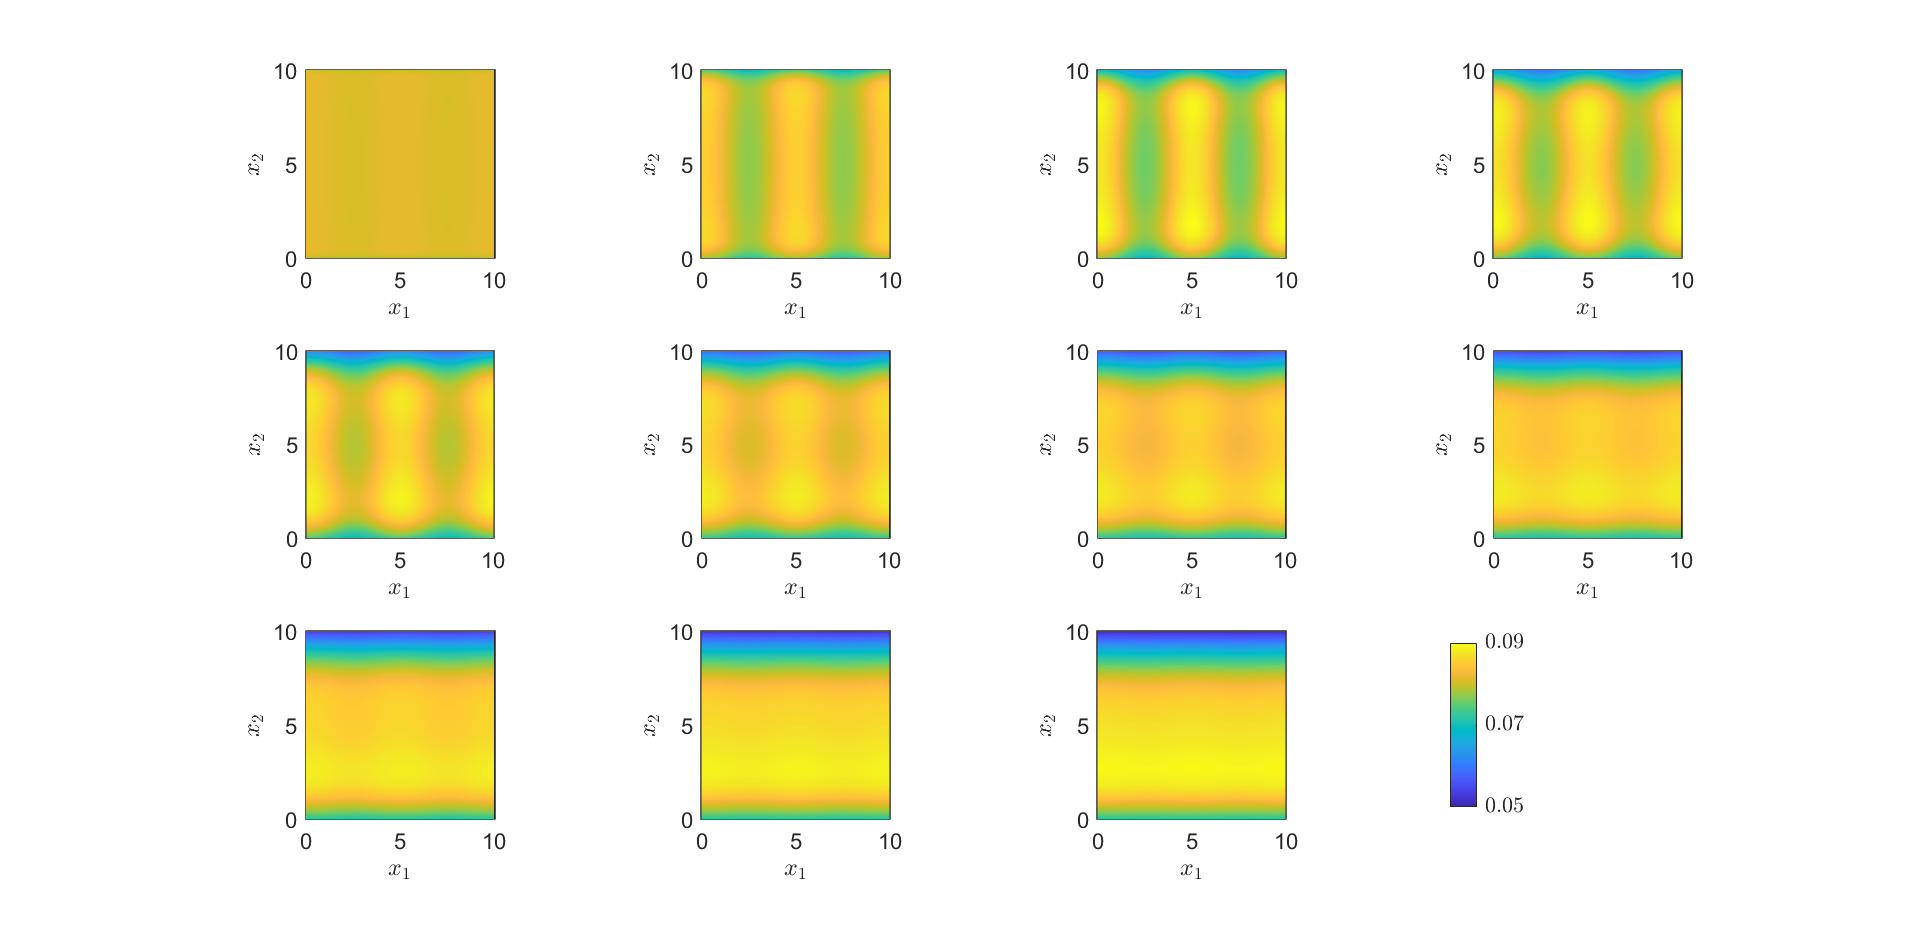
\includegraphics[scale=0.35]{rhoOptPeri3a.png}
	\caption{Examples Section \ref{sec:PeriodicNoFlux1}: Optimal state $\rho$ in periodic box} 
	\label{F4i}
\end{figure}

\begin{figure}[h]
	\centering
	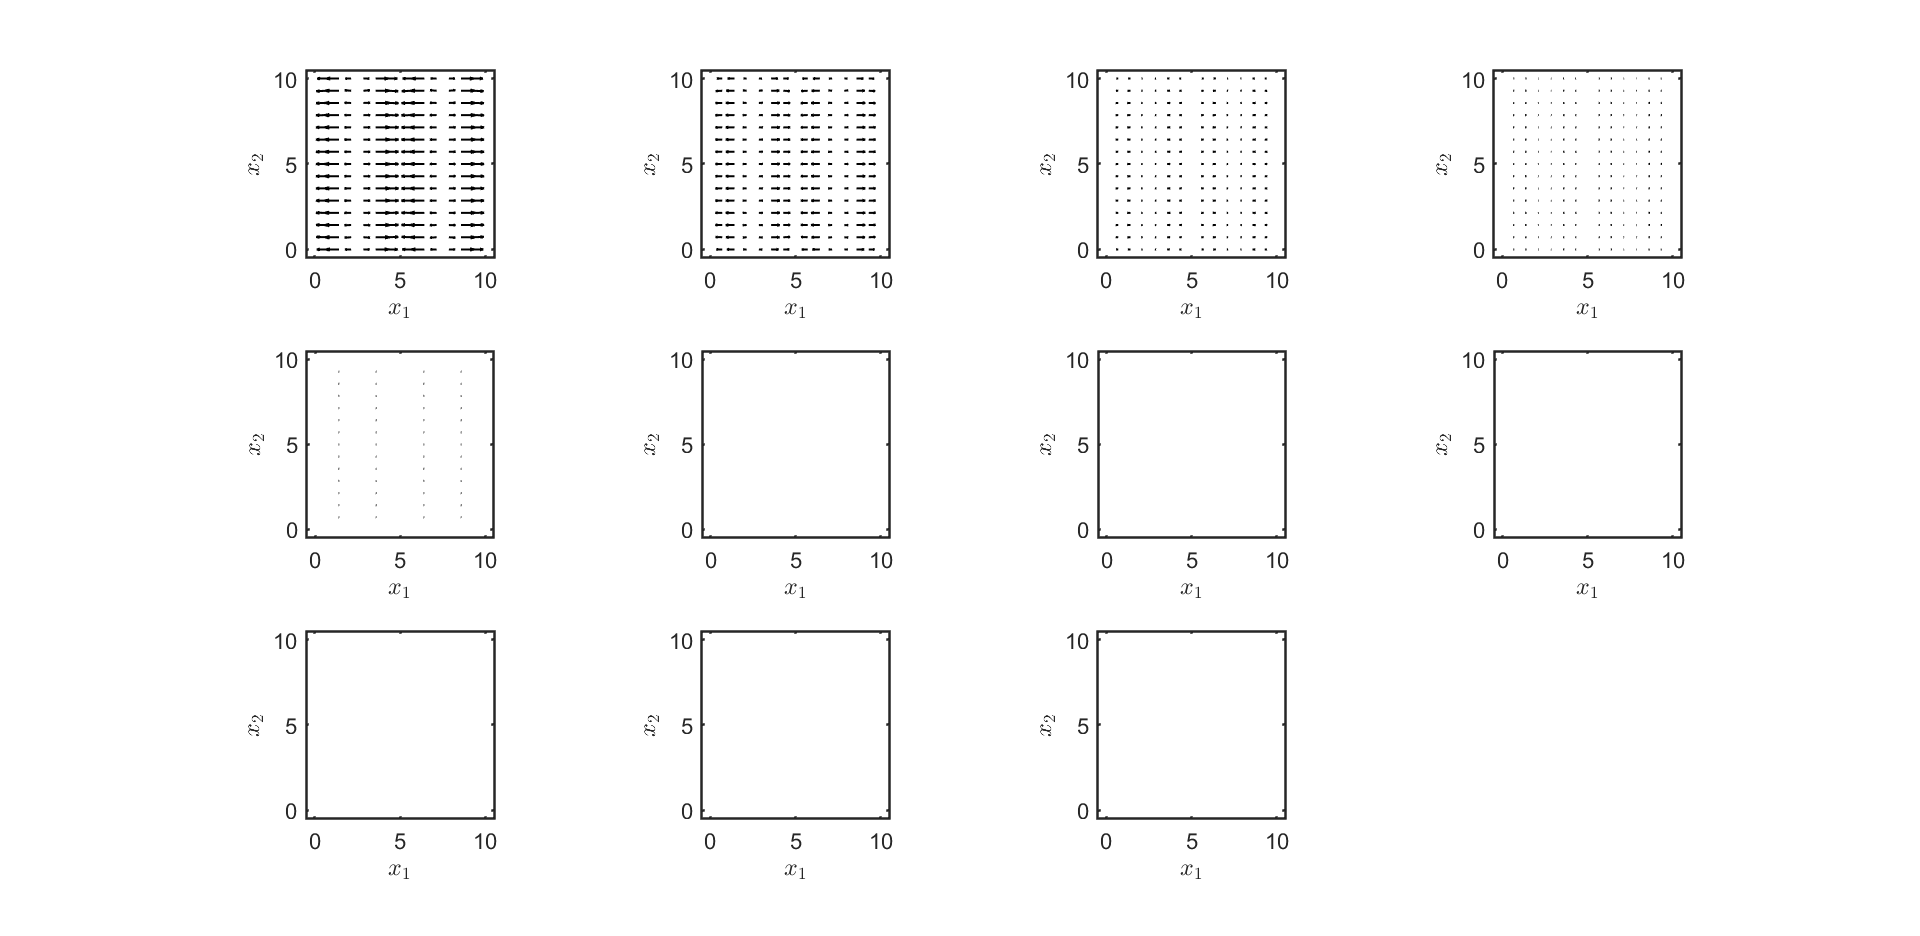
\includegraphics[scale=0.35]{ConOptPeri3a.png}
	\caption{Examples Section \ref{sec:PeriodicNoFlux1}: Optimal control corresponding to optimal state in Figure \ref{F4i}.} 
	\label{F4j}
\end{figure}



\subsection{Comparing control action in no-flux and periodic problems when varying $V_{ext}$} \label{sec:PeriodicNoFlux2}
(SedPeriodicvsNoFluxOCP)
We choose a domain $[0,15] \times [0,20]$ with $N = 30$ and a time horizon $(0,3)$ with $n = 30$. We choose the initial condition for $\rho$ to be uniform $\rho_0 = 0.1$. The interaction potential is of strength $\kappa = -3.5$. We set all other tolerances as in the previous section.
We are interested in setting up a target on a periodic box with external potential strength $a = 0.1$. We then set up the optimal control problem with $a =0$. We are interested in whether the optimal control can perform better than the external potential.

We get $\mathcal J_{FW} =  0.0082$ and $\mathcal J_{Opt} =  0.0023$. The results can be seen in Figures \ref{F5a} and \ref{F5b}. The target for this problem can be seen in Figure \ref{F5} and $-\nabla V_{ext}$ in Figure \ref{F5V}. This should be compared to the optimal control in Figure \ref{F5b}. We can compare the $L_2$ in space, $L_1$ in time norm, denoted by $N$, for the control and the negative gradient for $V_{ext}$, which is equivalent to comparing the second term in the cost functional for each case. We get that $N_{-\nabla V_{ext}} = 9$ and $N_{\w} = 2.9449$, which is considerably lower.

The same is done on a periodic box. We get $\mathcal J_{FW} = 0.0081$ and $\mathcal J_{Opt} = 0.0023$. The results can be seen in Figures \ref{F6a} and \ref{F6b}. The target for this is displayed in Figure \ref{F6} and $- \nabla V_{ext}$ is displayed in Figure \ref{F6V}, which should be compared to the optimal control in Figure \ref{F6b}. We can compare the norm for the control and the negative gradient for $V_{ext}$ again. We get that $N_{-\nabla V_{ext}} = 9$ and $N_{\w} = 2.9386$, which is considerably lower.

\begin{figure}[h]
	\centering
	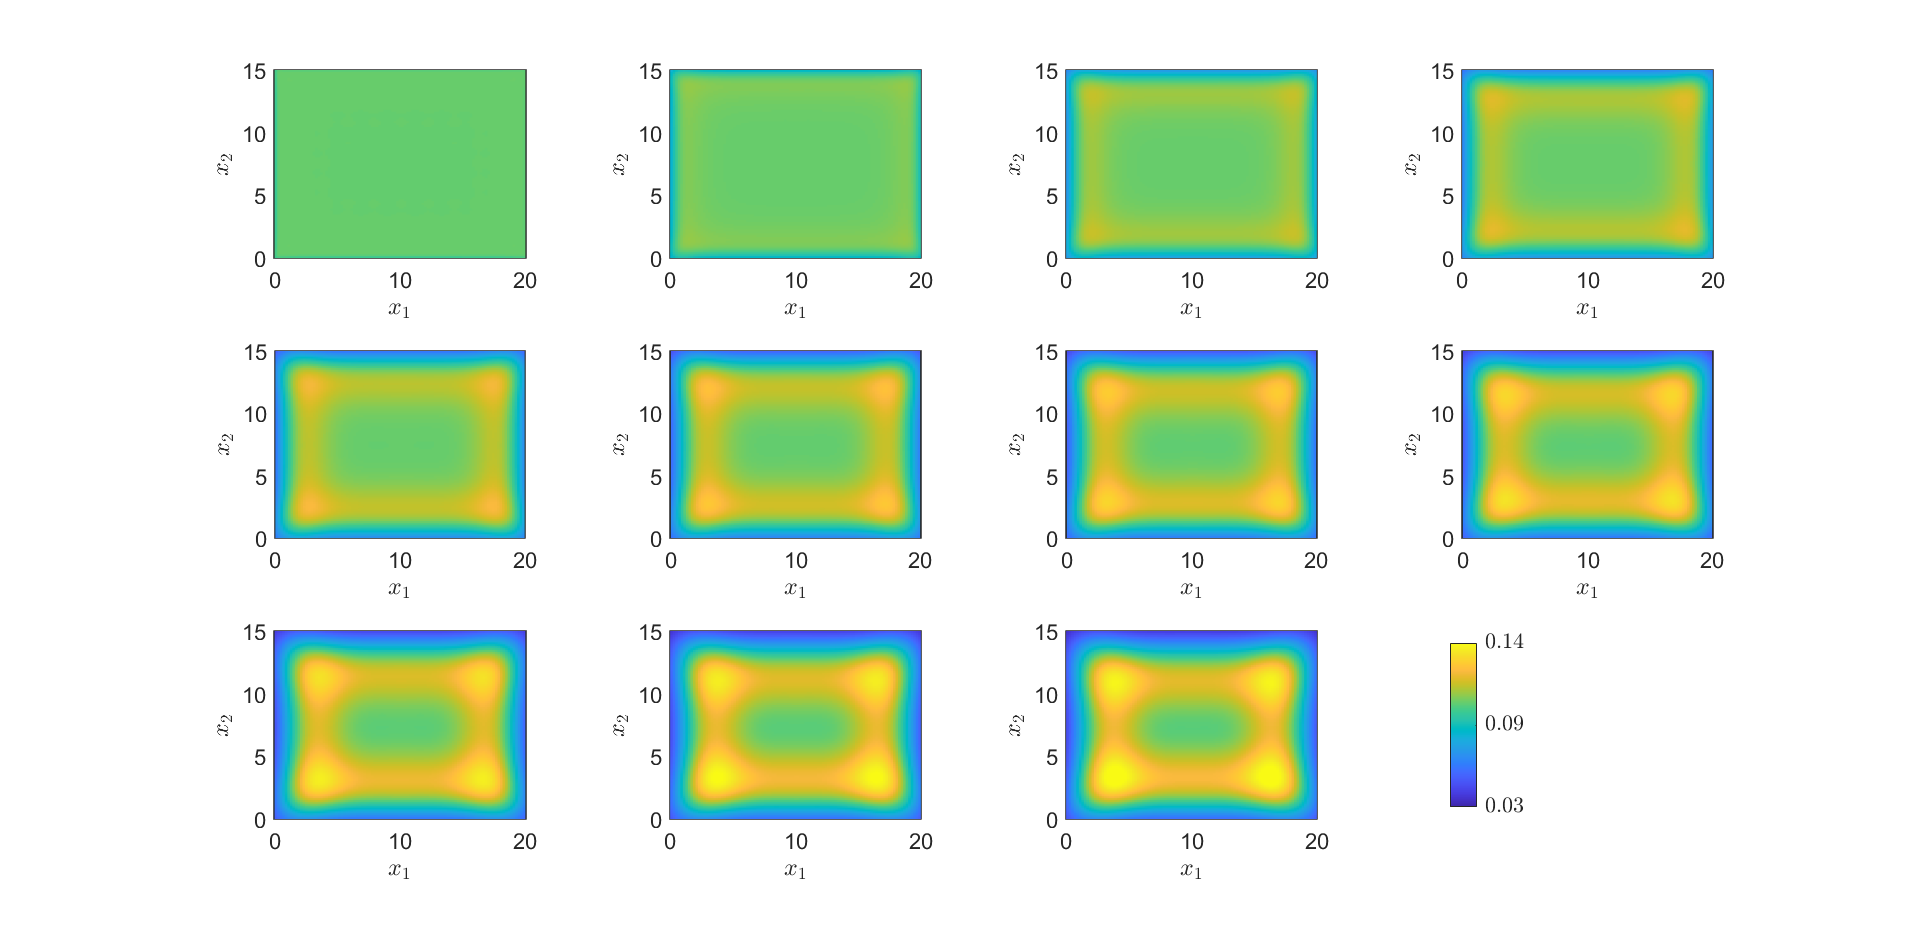
\includegraphics[scale=0.35]{rhoHatPeri5.png}
	\caption{Examples Section \ref{sec:PeriodicNoFlux2}: $\hr$ created in a no-flux box with $a = 0.1$ corresponding to optimal state in Figure \ref{F5a}.} 
	\label{F5}
\end{figure}
\begin{figure}[h]
	\centering
	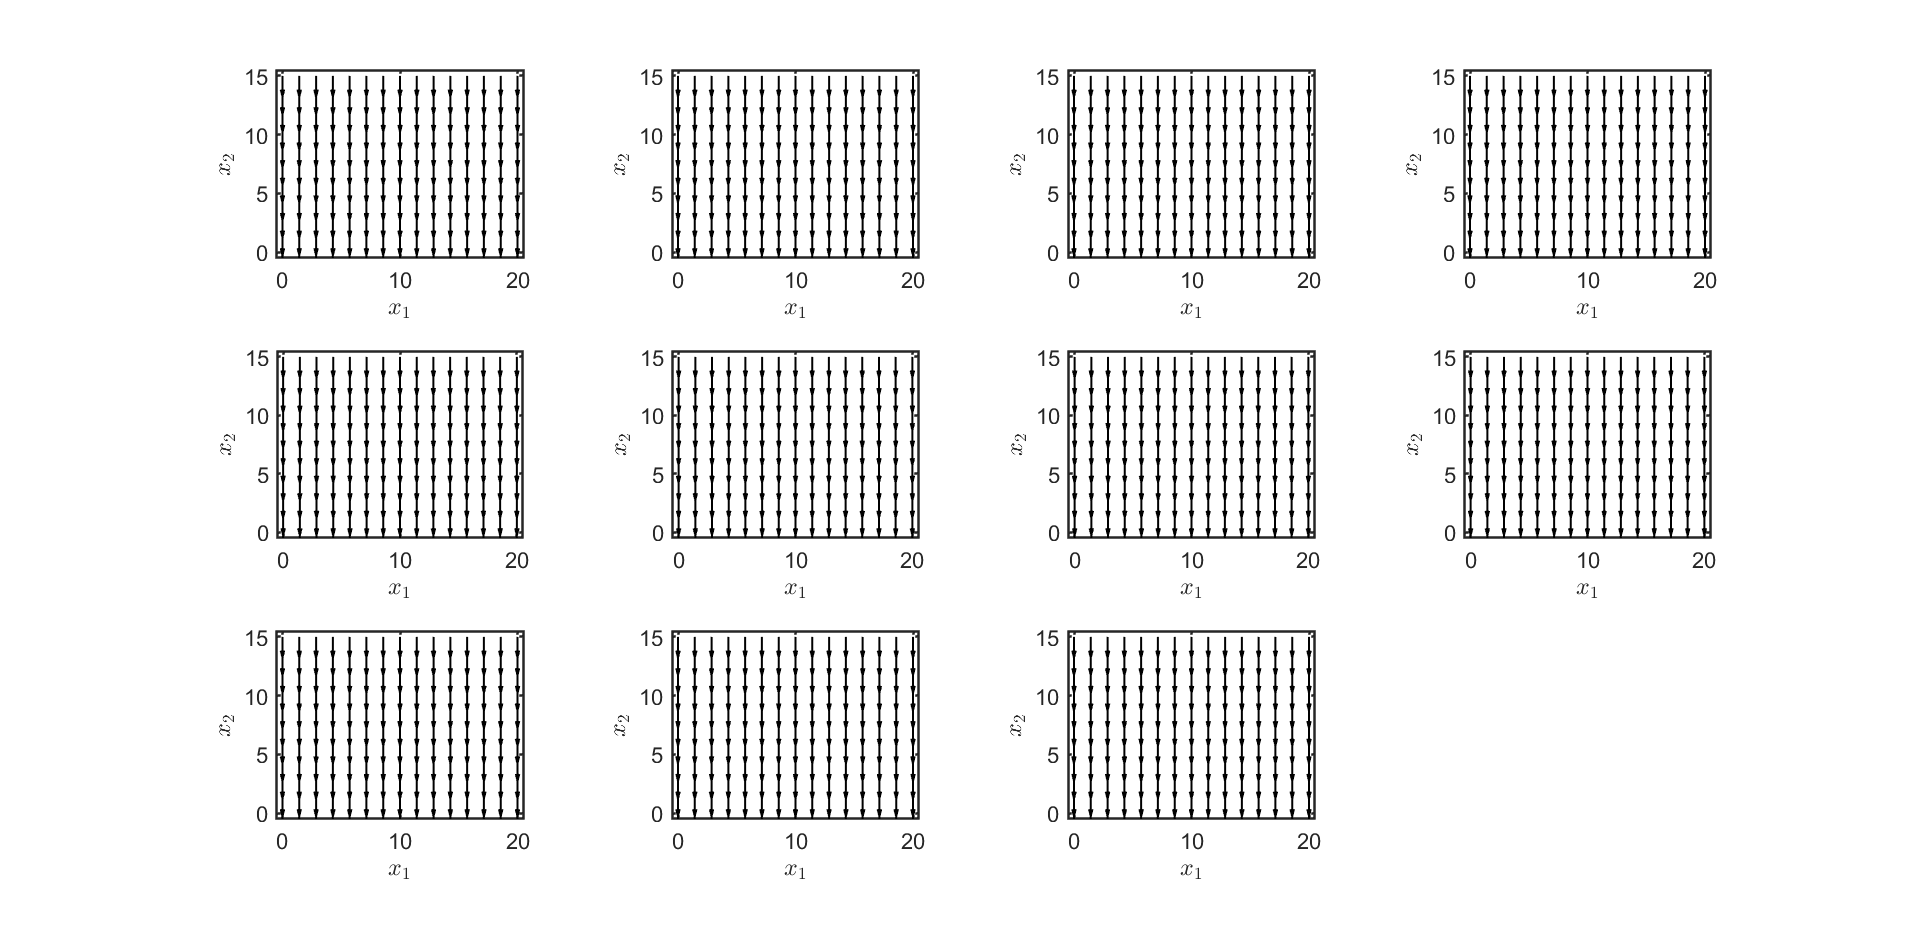
\includegraphics[scale=0.35]{GradVext5.png}
	\caption{Examples Section \ref{sec:PeriodicNoFlux2}: $-\nabla Vext$ with $a = 0.1$ corresponding to $\hr$ in Figure \ref{F5}. This can be compared to the optimal control displayed in Figure \ref{F5b}.} 
	\label{F5V}
\end{figure}
\begin{figure}[h]
	\centering
	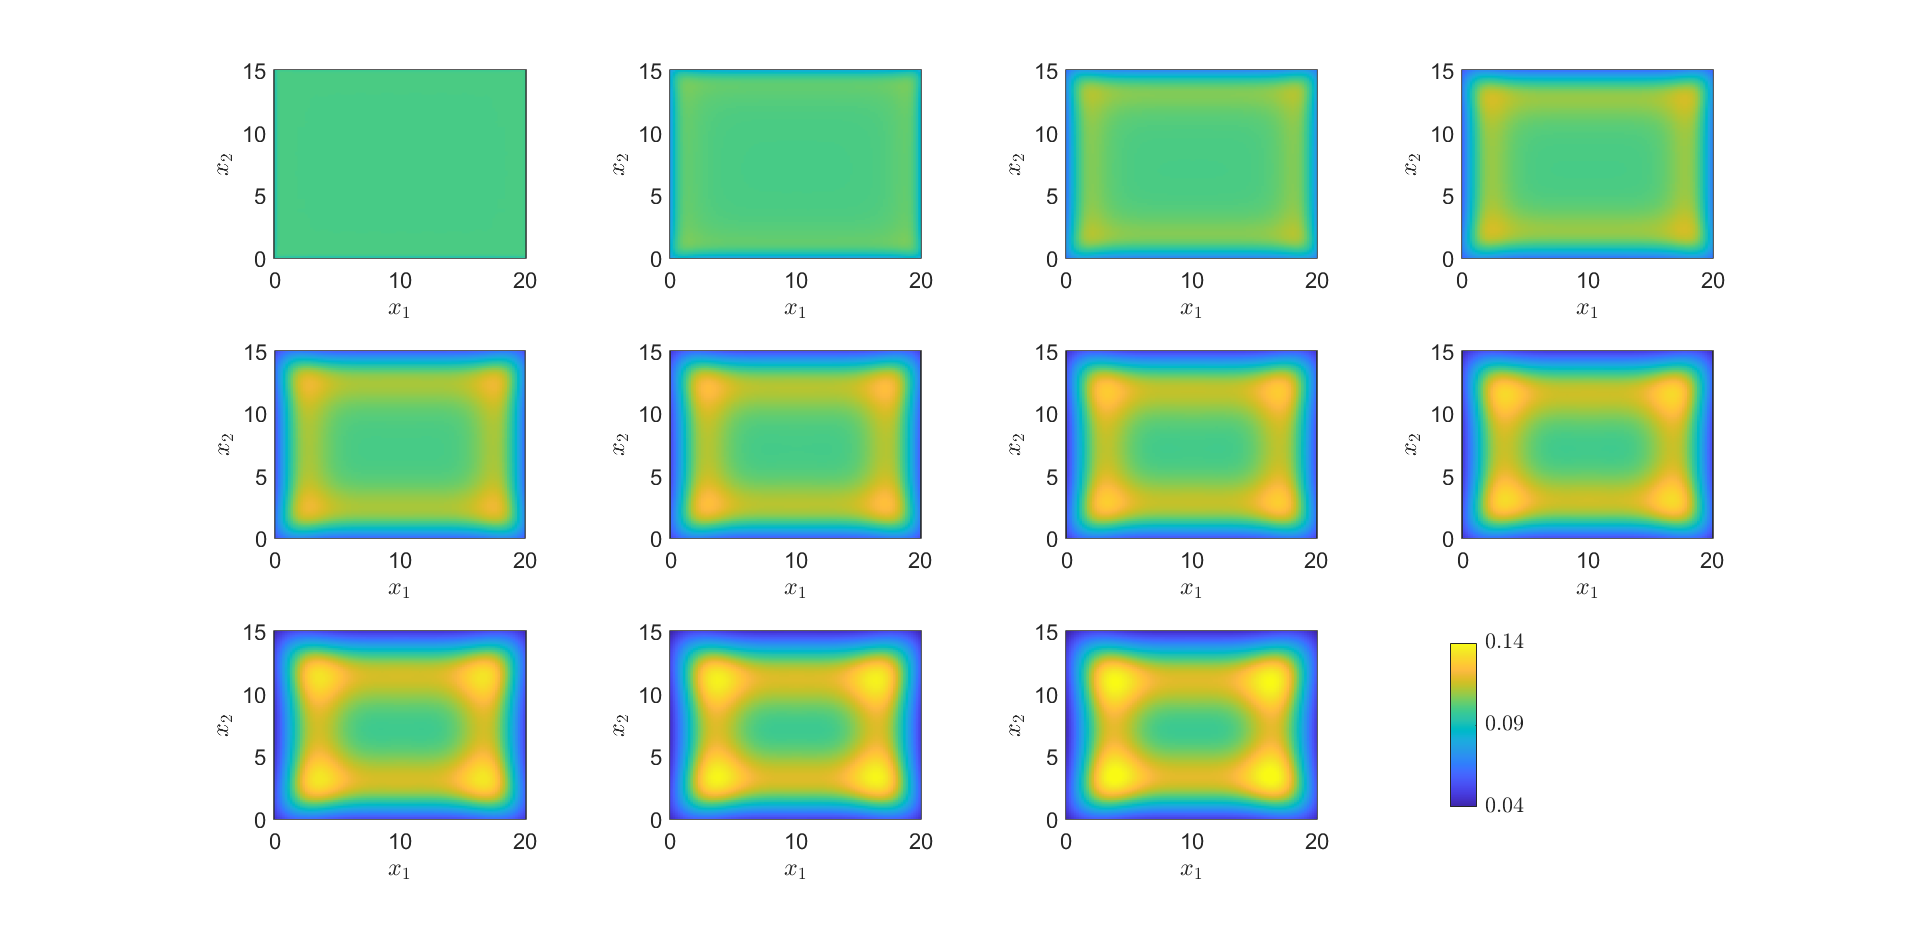
\includegraphics[scale=0.35]{rhoOptPeri5.png}
	\caption{Examples Section \ref{sec:PeriodicNoFlux2}: Optimal state $\rho$ in a no-flux box, with $a = 0$} 
	\label{F5a}
\end{figure}

\begin{figure}[h]
	\centering
	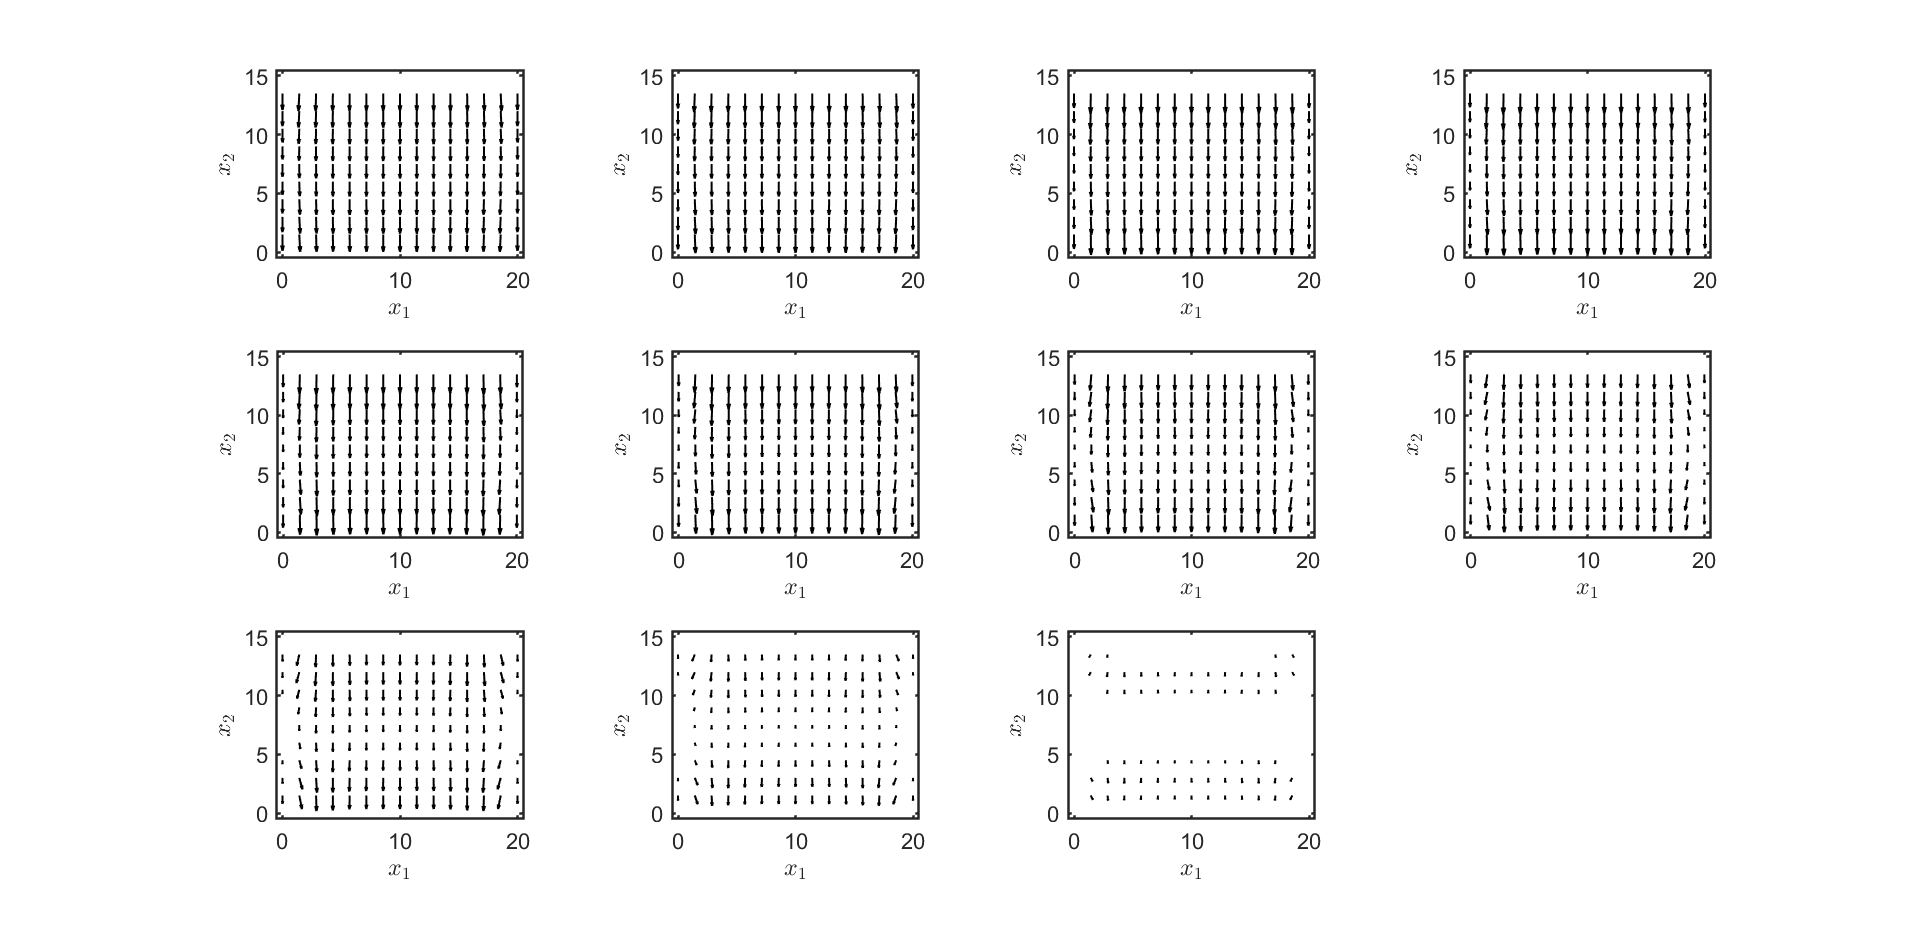
\includegraphics[scale=0.35]{ConOptPeri5.png}
	\caption{Examples Section \ref{sec:PeriodicNoFlux2}: Optimal control corresponding to optimal state in Figure \ref{F5a}.} 
	\label{F5b}
\end{figure}



\begin{figure}[h]
	\centering
	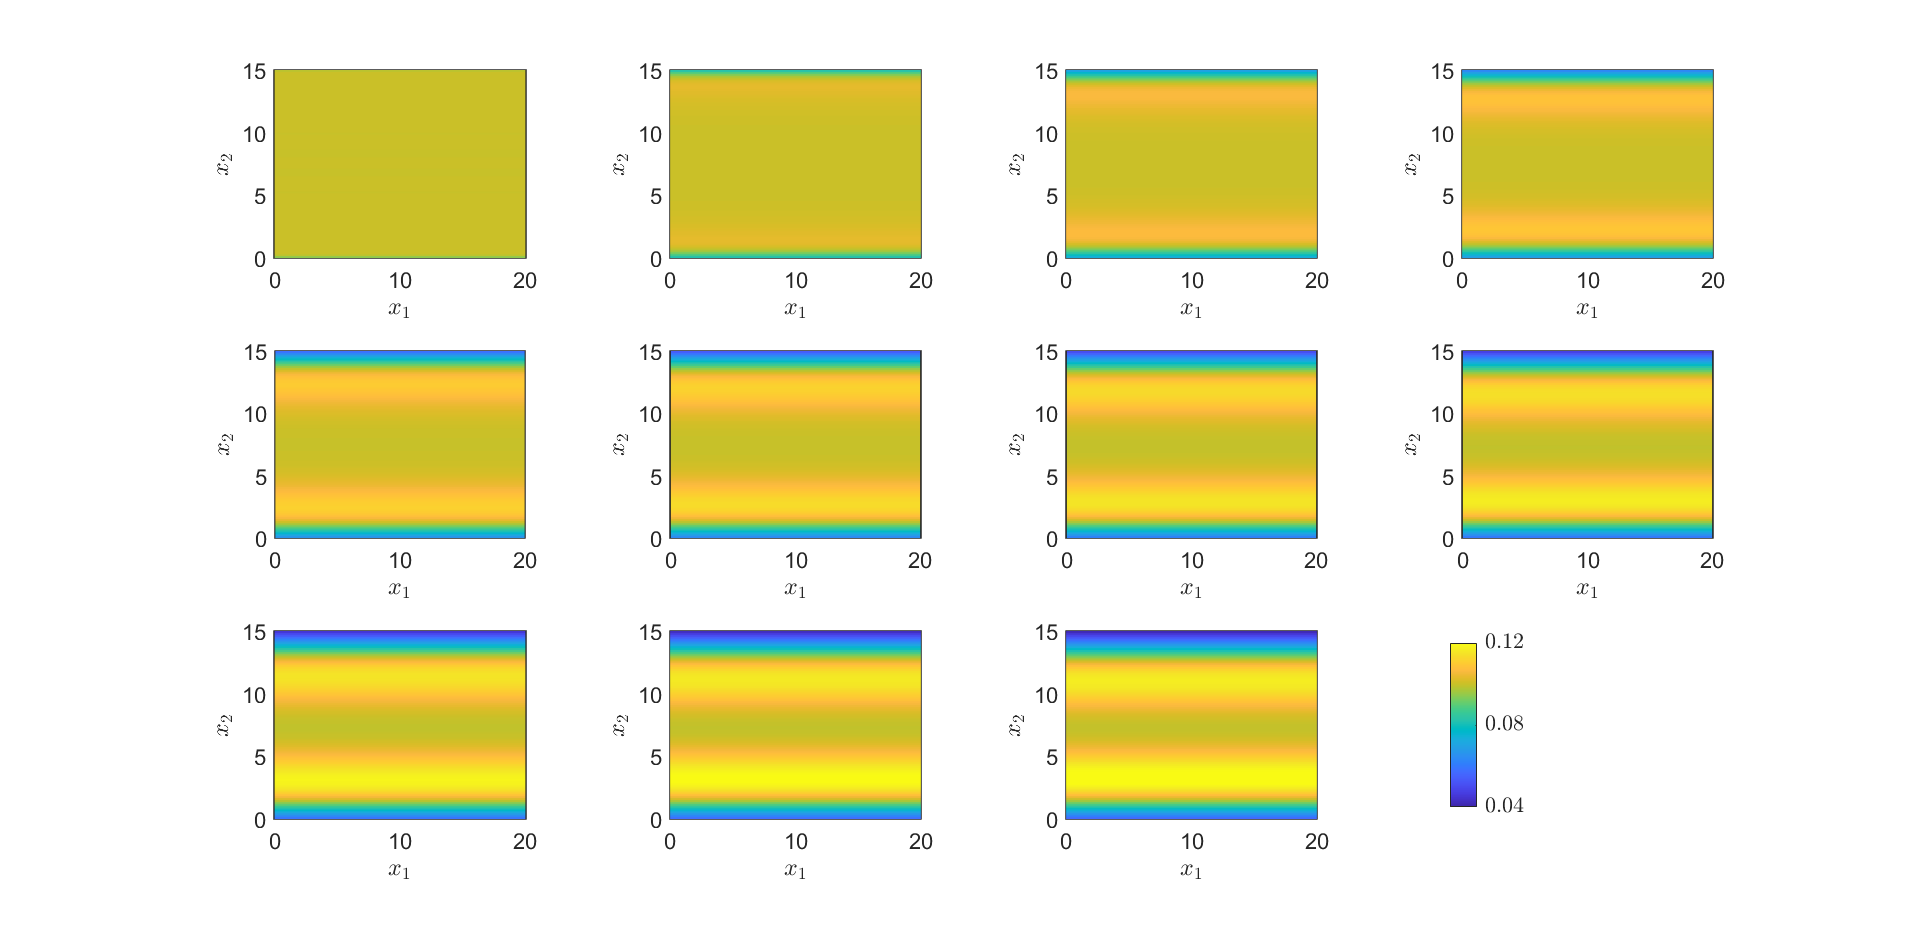
\includegraphics[scale=0.35]{rhoHatPeri6.png}
	\caption{Examples Section \ref{sec:PeriodicNoFlux2}: $\hr$ created in a periodic box with $a = 0.1$ corresponding to optimal state in Figure \ref{F6a}.} 
	\label{F6}
\end{figure}
\begin{figure}[h]
	\centering
	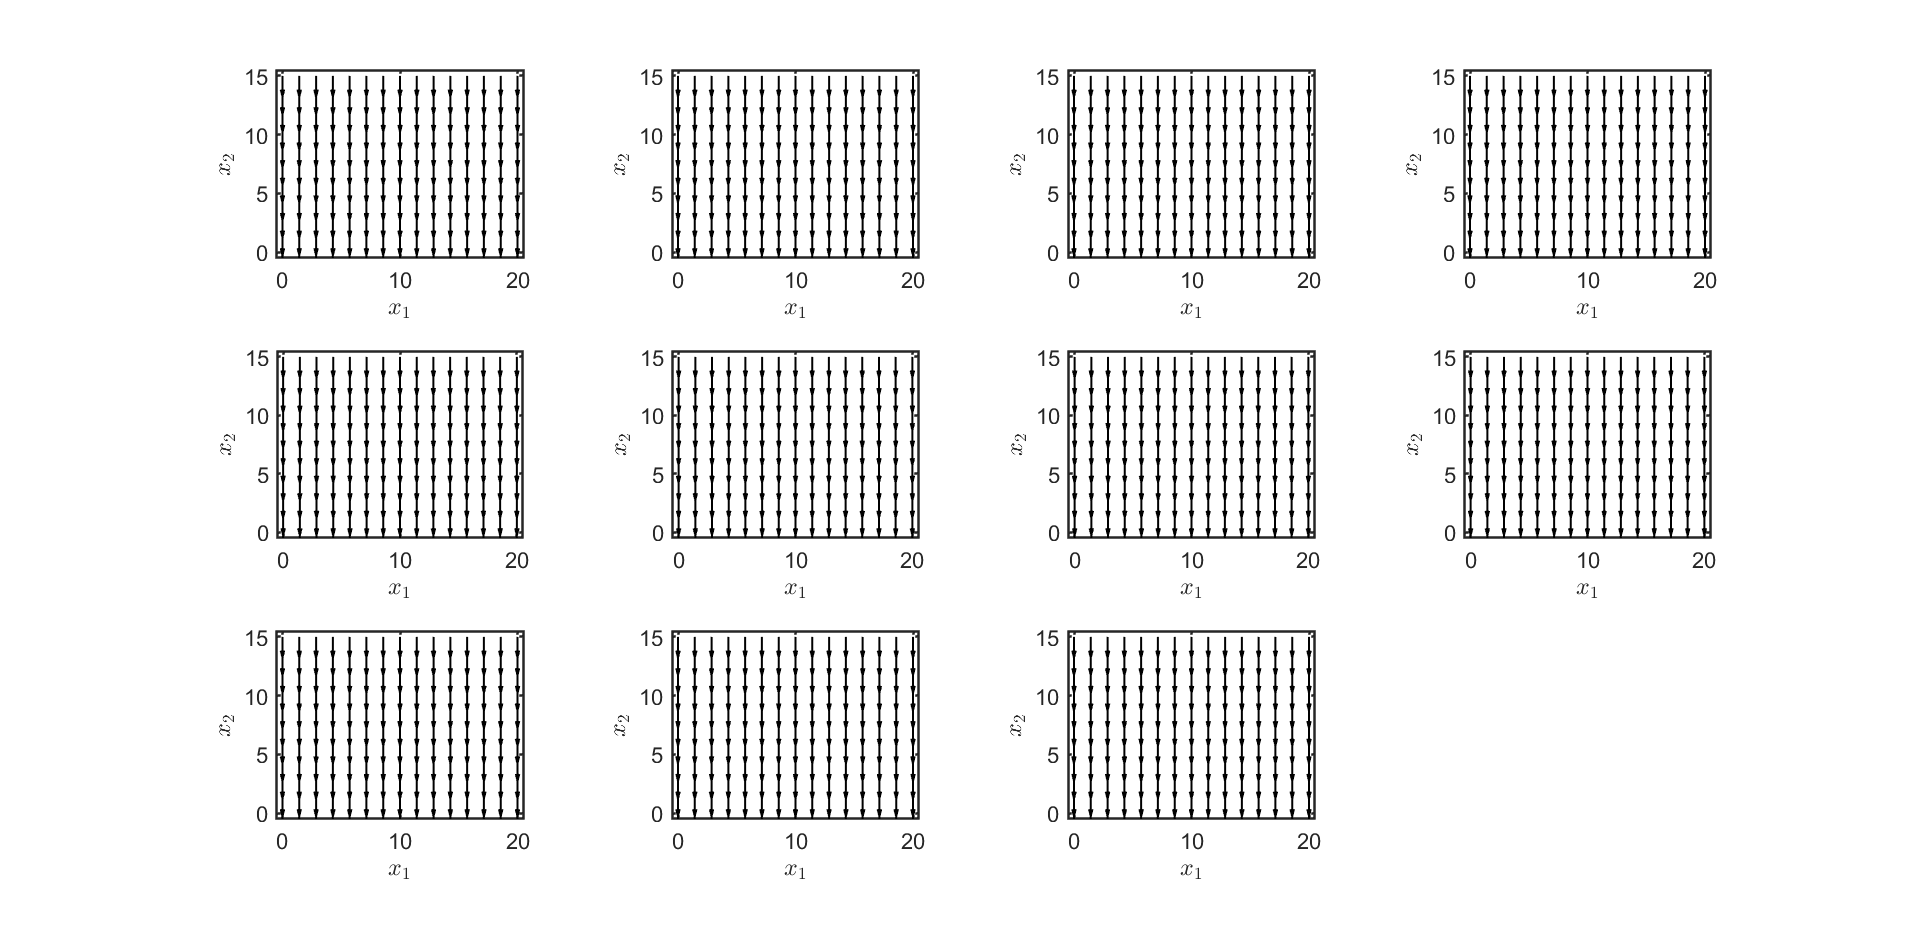
\includegraphics[scale=0.35]{GradVext6.png}
	\caption{Examples Section \ref{sec:PeriodicNoFlux2}: $-\nabla Vext$ with $a = 0.1$ corresponding to $\hr$ in Figure \ref{F6}. This can be compared to the optimal control displayed in Figure \ref{F6b}.} 
	\label{F6V}
\end{figure}
\begin{figure}[h]
	\centering
	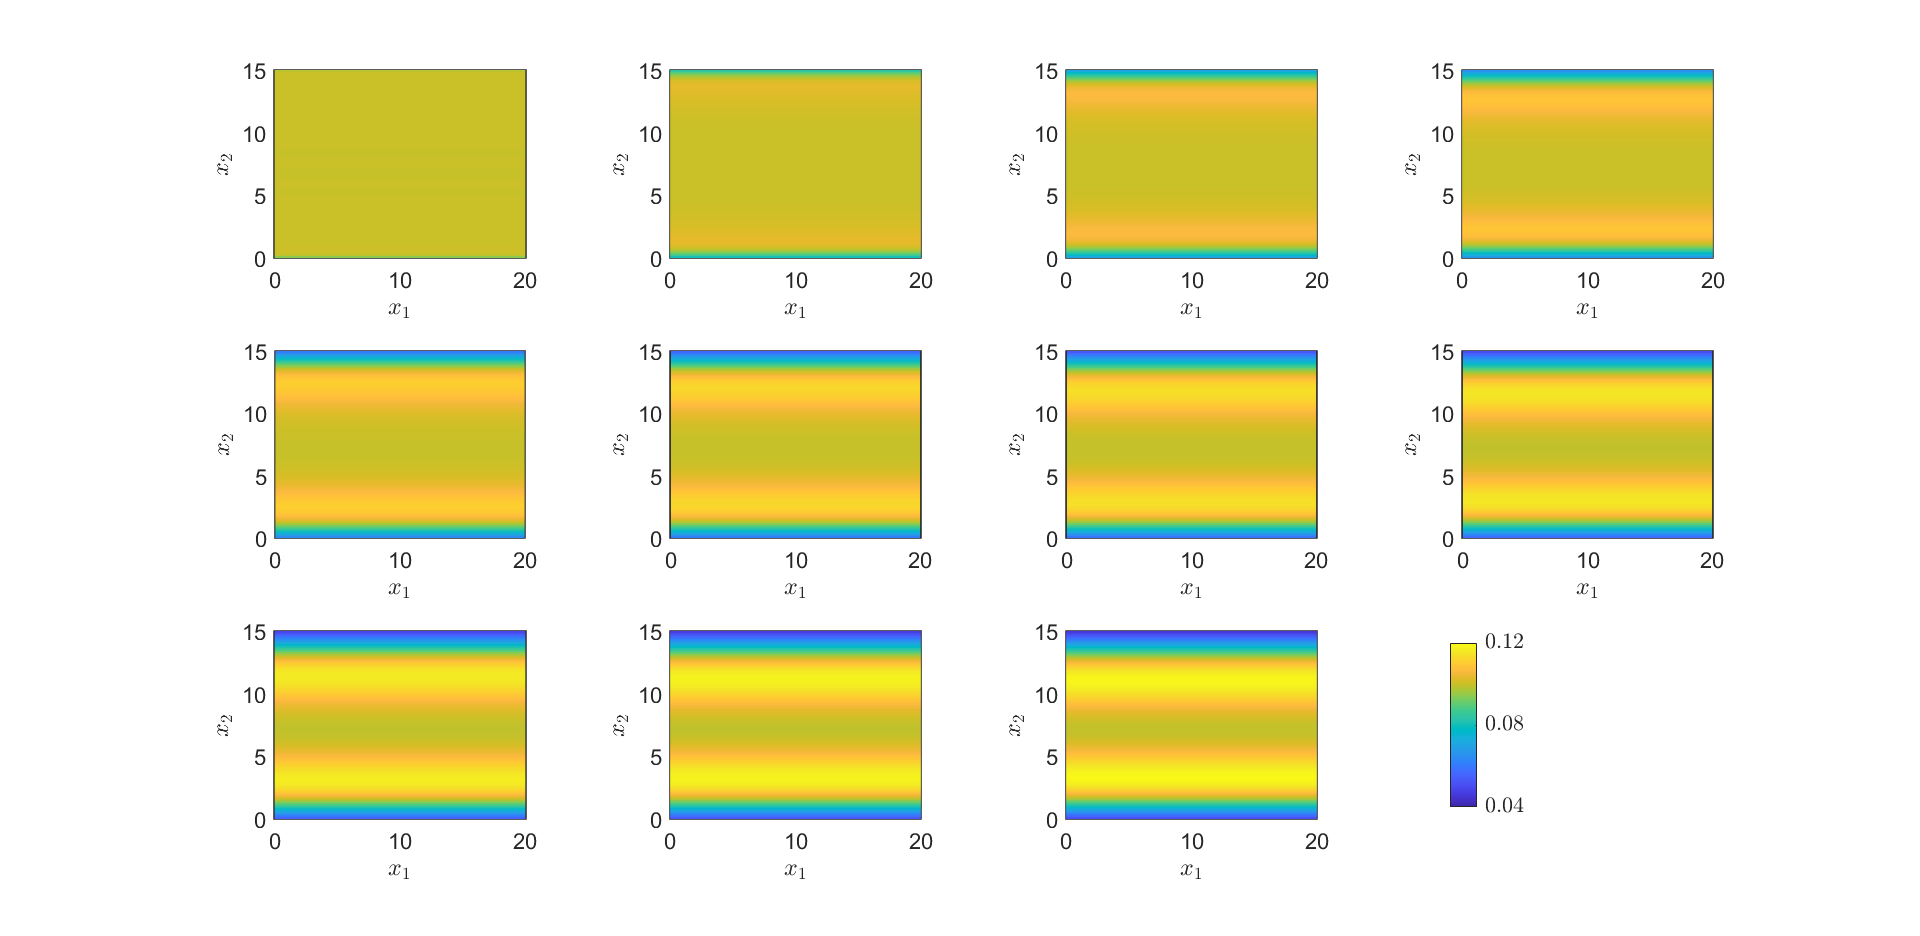
\includegraphics[scale=0.35]{rhoOptPeri6.png}
	\caption{Examples Section \ref{sec:PeriodicNoFlux2}: Optimal state $\rho$ in a periodic box, with $a = 0$} 
	\label{F6a}
\end{figure}

\begin{figure}[h]
	\centering
	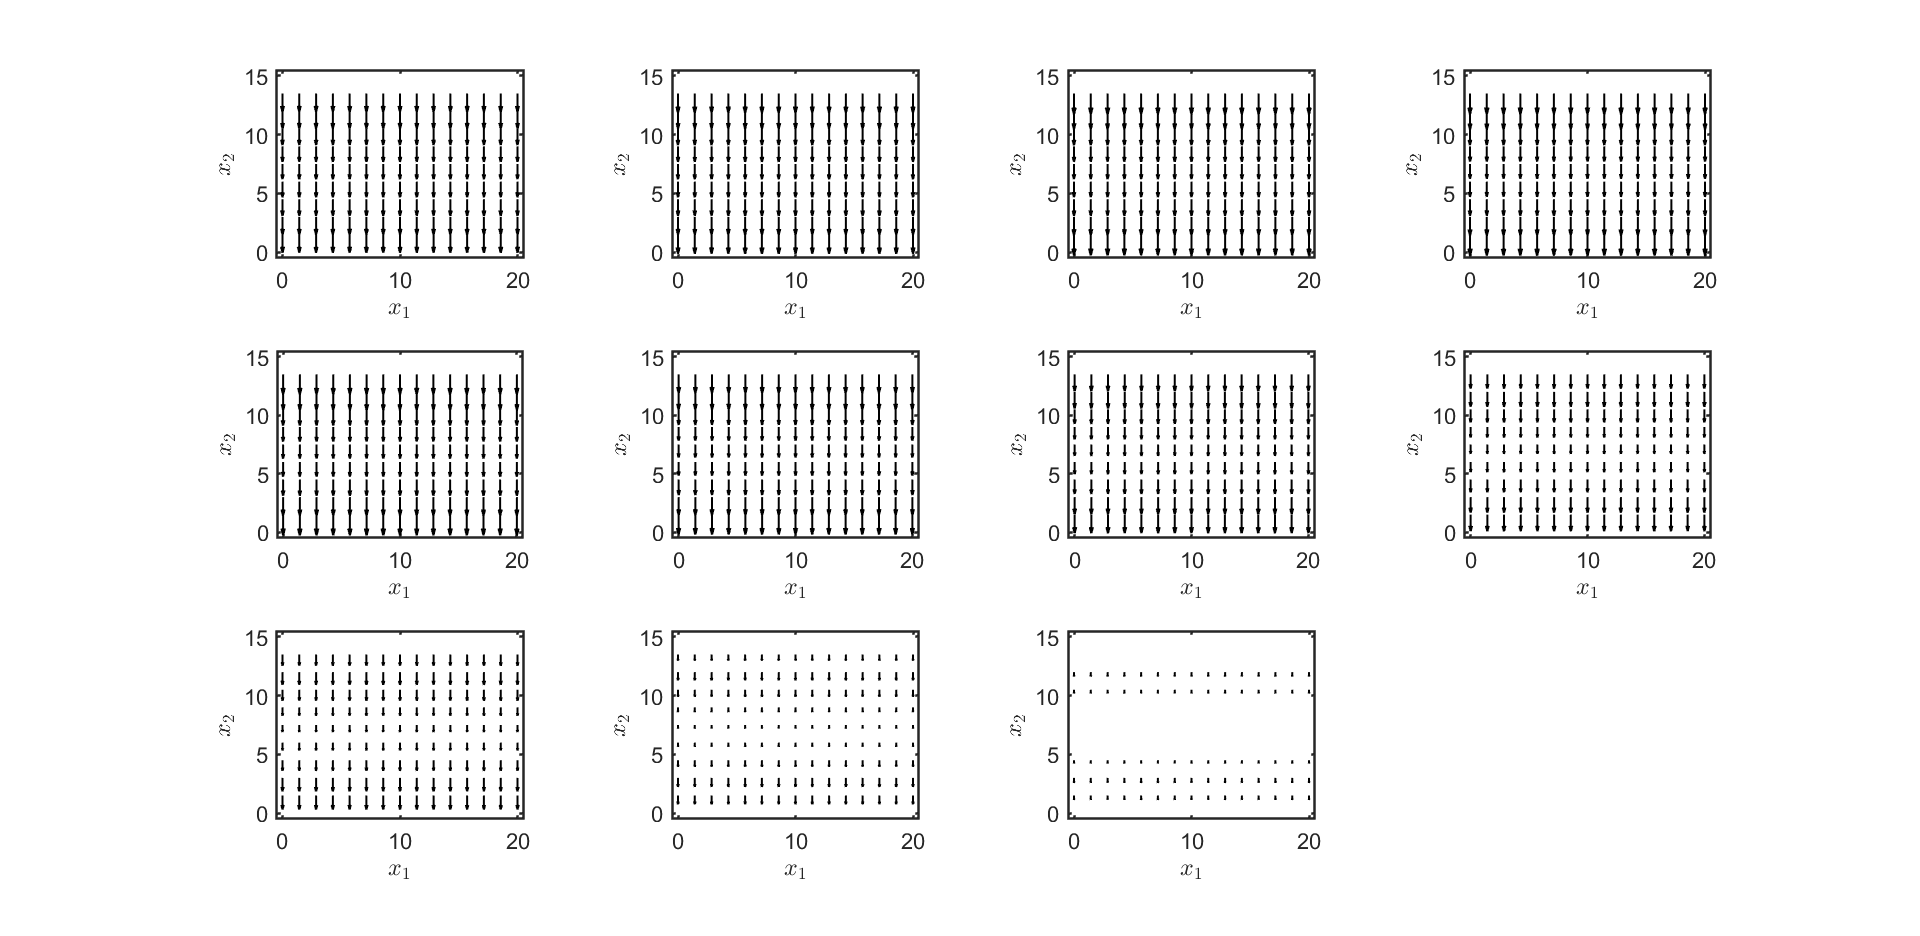
\includegraphics[scale=0.35]{ConOptPeri6.png}
	\caption{Examples Section \ref{sec:PeriodicNoFlux2}: Optimal control corresponding to optimal state in Figure \ref{F6a}.} 
	\label{F6b}
\end{figure}


\subsection{Comparing the effect of interactions} \label{sec:PeriodicNoFlux3}
(SedPeriodicOCP/SedNoFluxOCP)
Finally we are interested in the effects of computing a problem in a no-flux and periodic box when we change the interaction strengths between the target and the dynamics of the problem.
We set all parameters as in the previous section. One difference is that the uniform initial condition for $\rho$ is perturbed by a random perturbation of strength $1/20 \rho_0$.

For the no-flux box we have a target with $\kappa = -3.5$, which is a forward problem forming clusters. The uncontrolled dynamics does not have particle interactions resent ($\kappa =0$). It is of interest how the optimal control acts to form clusters. The target is displayed in Figure \ref{F7} and the optimal state and control are displayed in Figures \ref{F7a} and \ref{F7b}. We get $\mathcal J_{FW} = 1.8380$ and $\mathcal J_{Opt} = 0.2005$.
\begin{figure}[h]
	\centering
	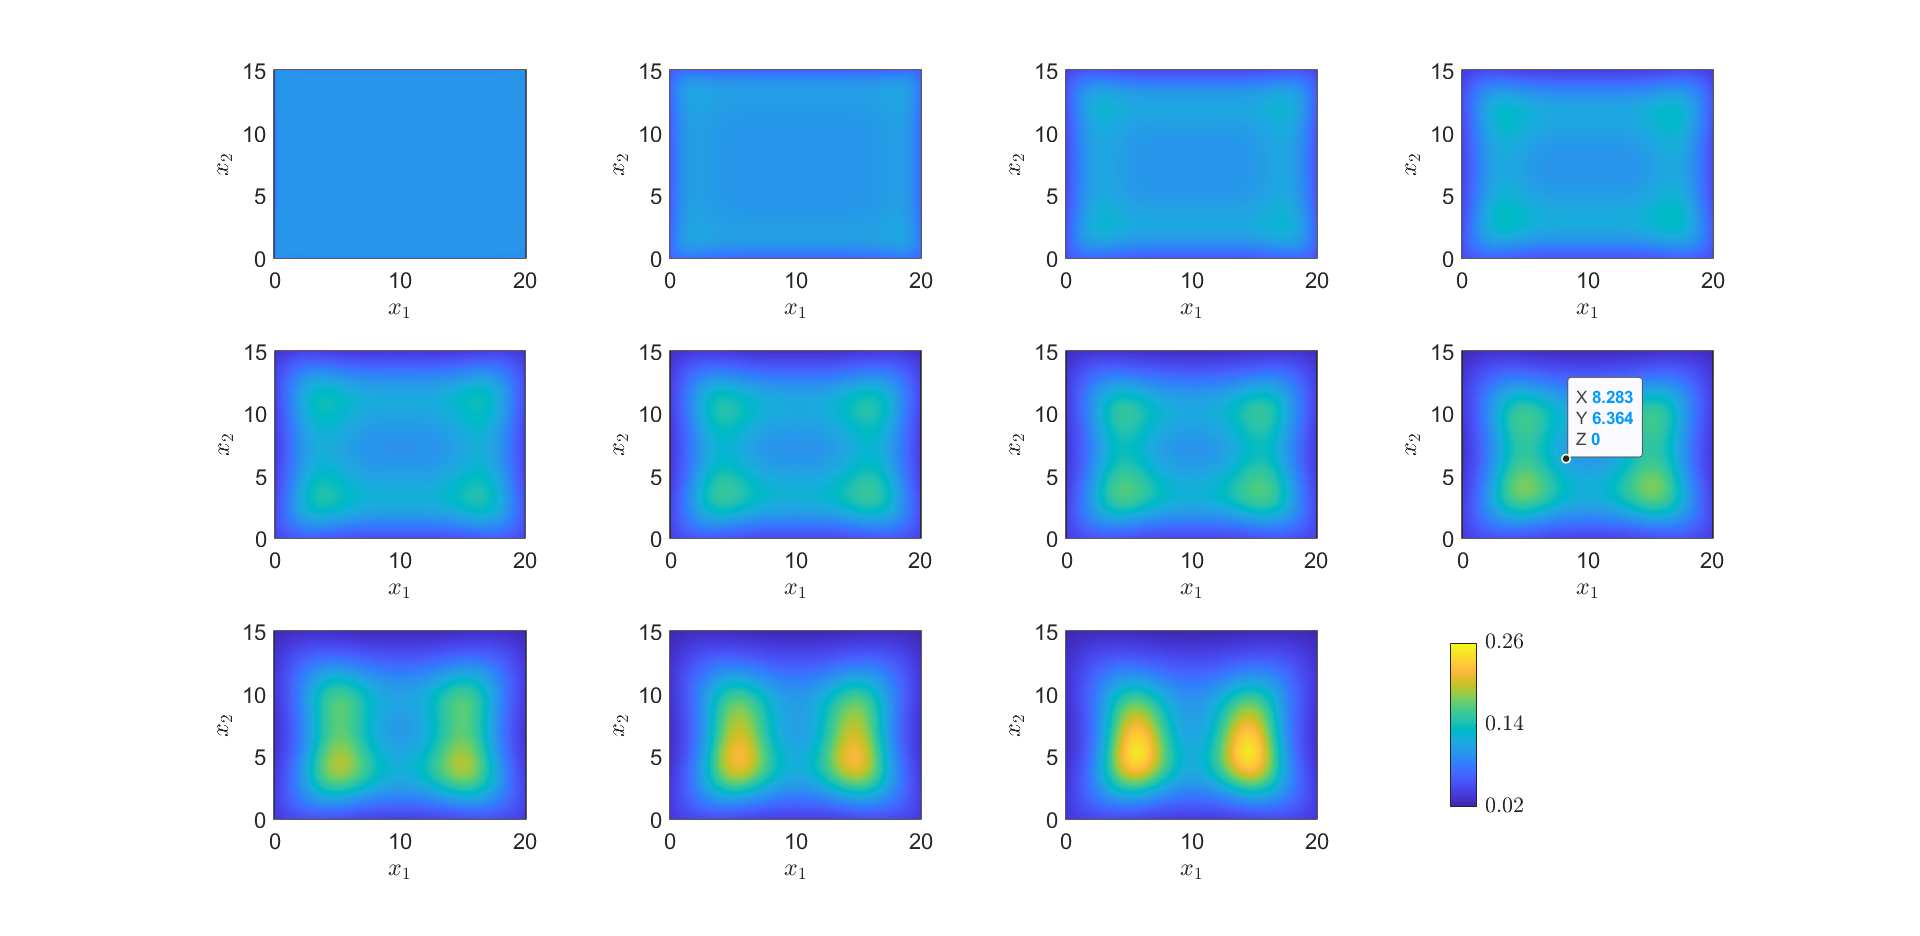
\includegraphics[scale=0.35]{rhoHatPeri7.png}
	\caption{Examples Section \ref{sec:PeriodicNoFlux3}: $\hr$ created in a no-flux box with $\kappa = -3.5$ corresponding to optimal state in Figure \ref{F7a}.} 
	\label{F7}
\end{figure}
\begin{figure}[h]
	\centering
	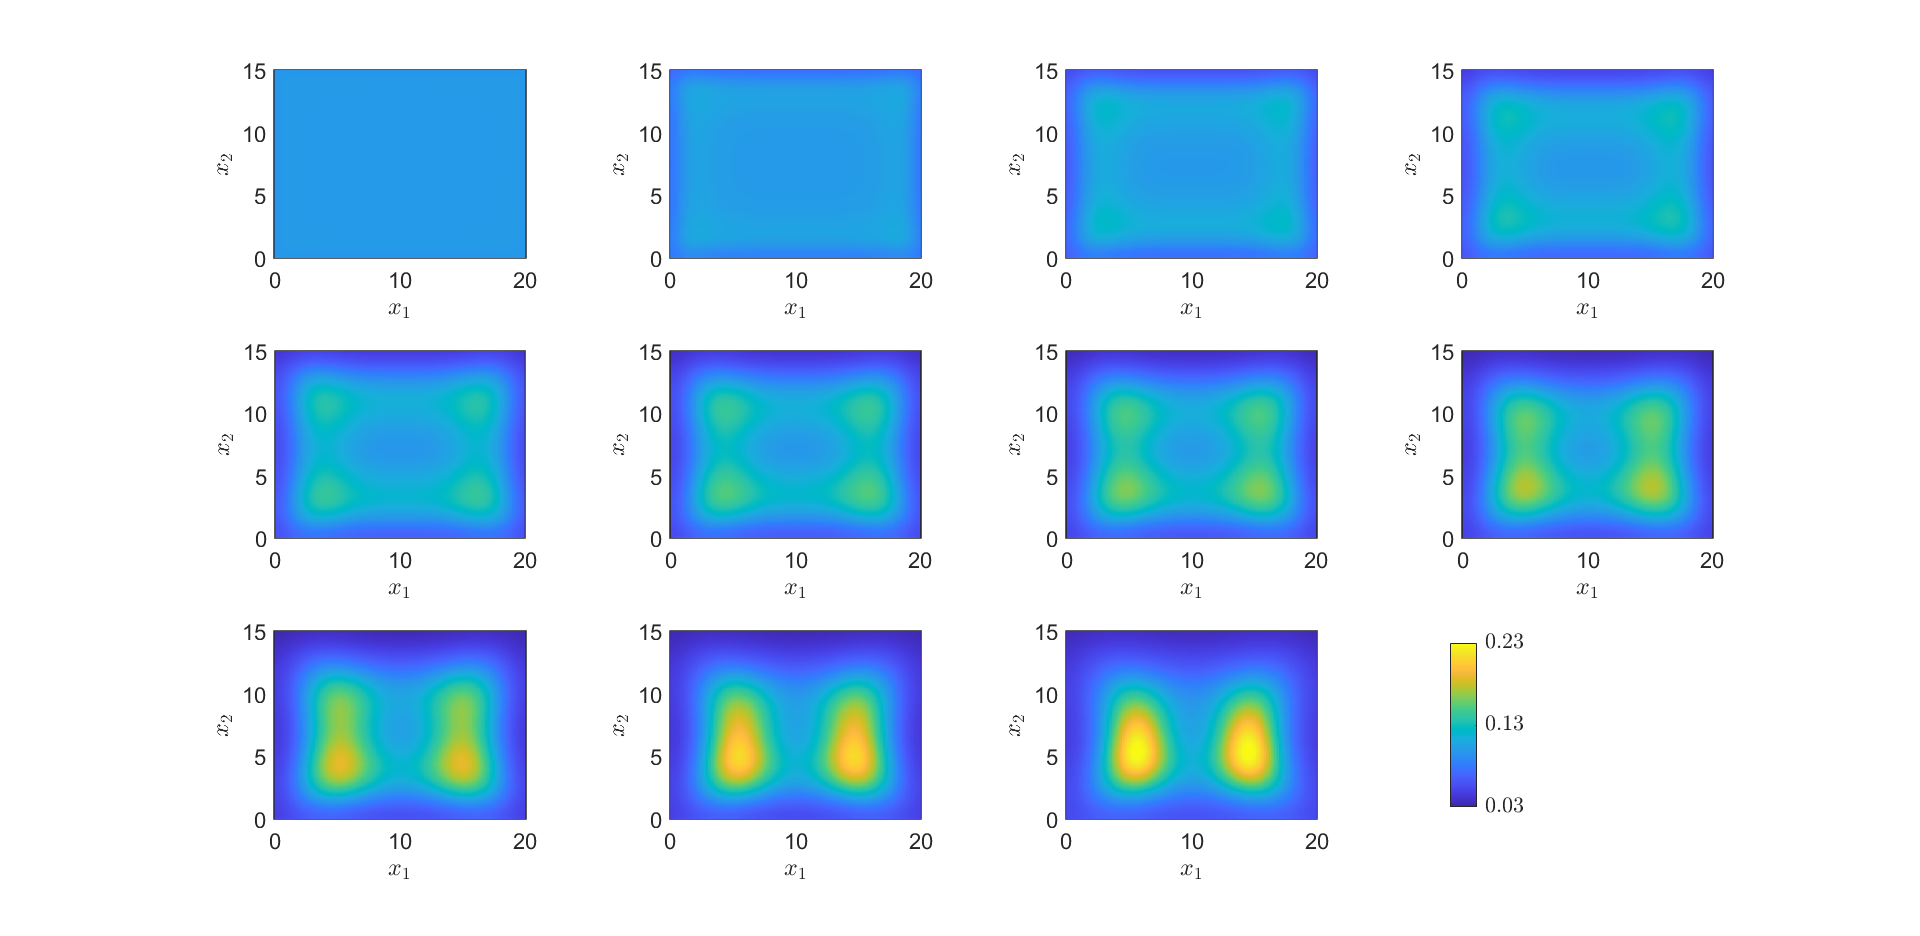
\includegraphics[scale=0.35]{rhoOptPeri7.png}
	\caption{Examples Section \ref{sec:PeriodicNoFlux3}: Optimal state $\rho$ in a no-flux box, with $\kappa = 0$} 
	\label{F7a}
\end{figure}

\begin{figure}[h]
	\centering
	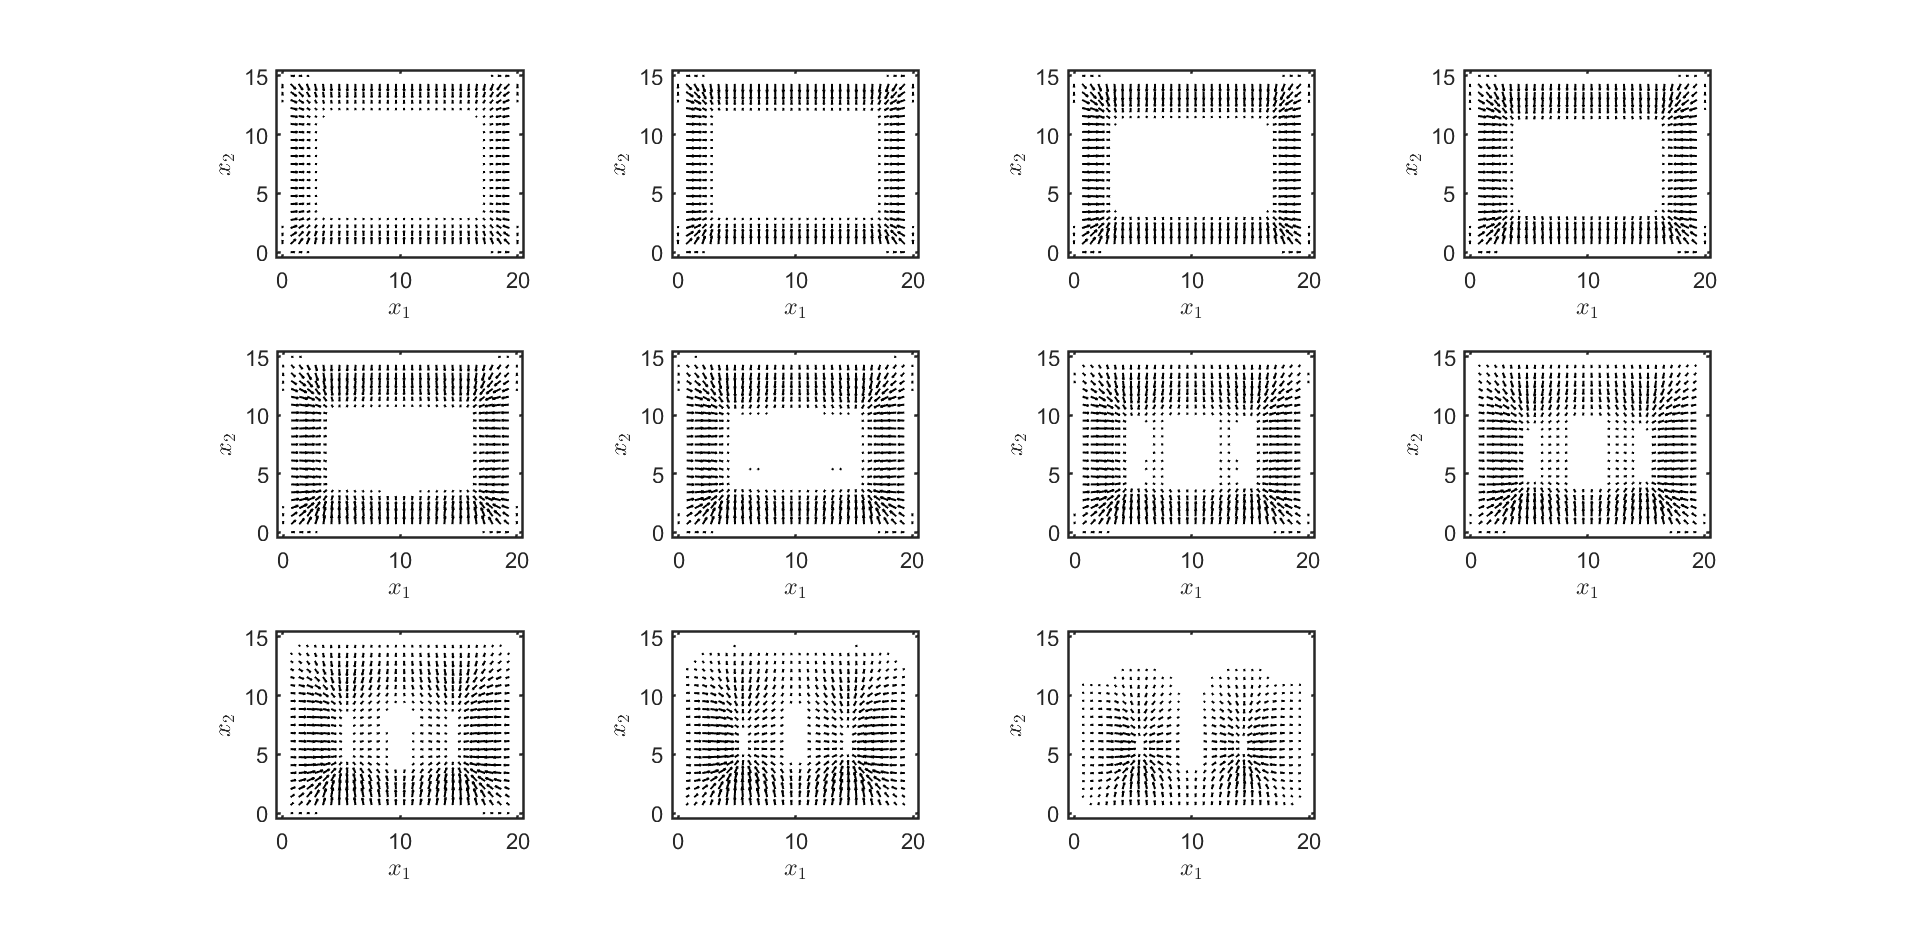
\includegraphics[scale=0.35]{ConOptPeri7.png}
	\caption{Examples Section \ref{sec:PeriodicNoFlux3}: Optimal control corresponding to optimal state in Figure \ref{F7a}.} 
	\label{F7b}
\end{figure}



For the periodic box we again have a target with $\kappa = -3.5$, which is a forward problem forming clusters. The uncontrolled dynamics does not have particle interactions resent ($\kappa =0$). It is of interest how the optimal control acts to form clusters. The target is displayed in Figure \ref{F8} and the optimal state and control are displayed in Figures \ref{F8a} and \ref{F8b}. We get $\mathcal J_{FW} = 0.8690$ and $\mathcal J_{Opt} = 0.1027$.
\begin{figure}[h]
	\centering
	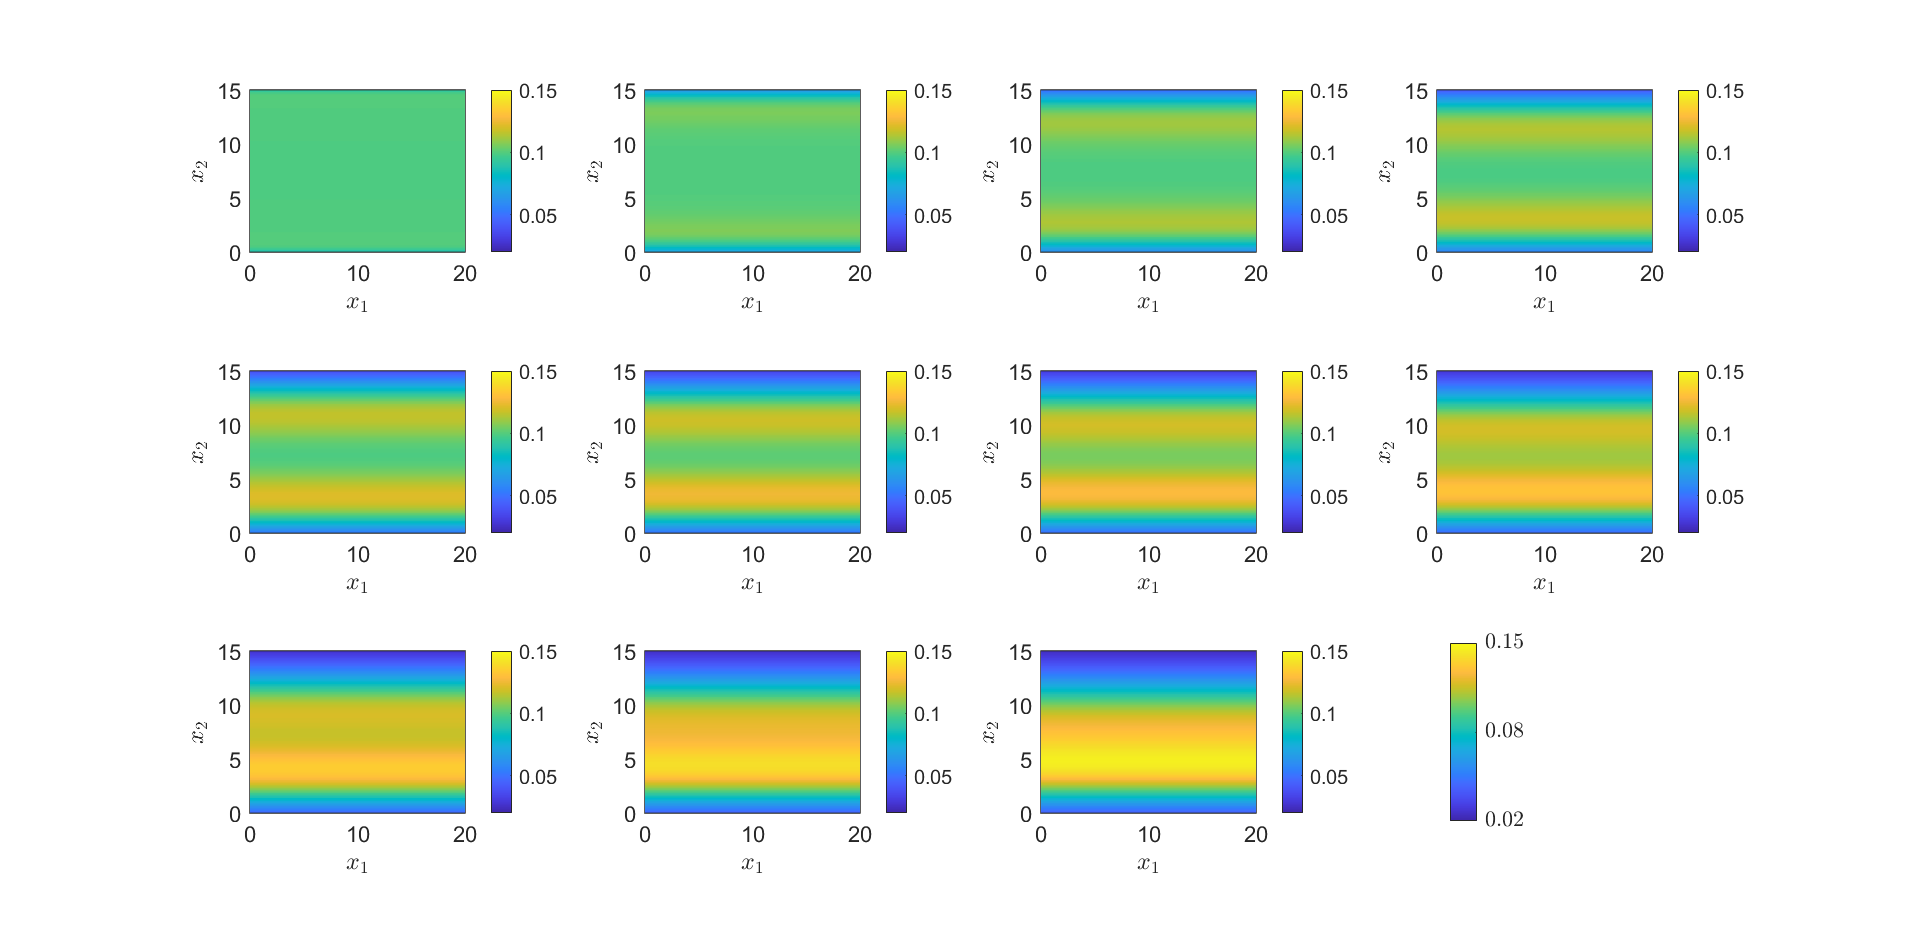
\includegraphics[scale=0.35]{rhoHatPeri8.png}
	\caption{Examples Section \ref{sec:PeriodicNoFlux3}: $\hr$ created in a periodic box with $\kappa = -3.5$ corresponding to optimal state in Figure \ref{F8a}.} 
	\label{F8}
\end{figure}
\begin{figure}[h]
	\centering
	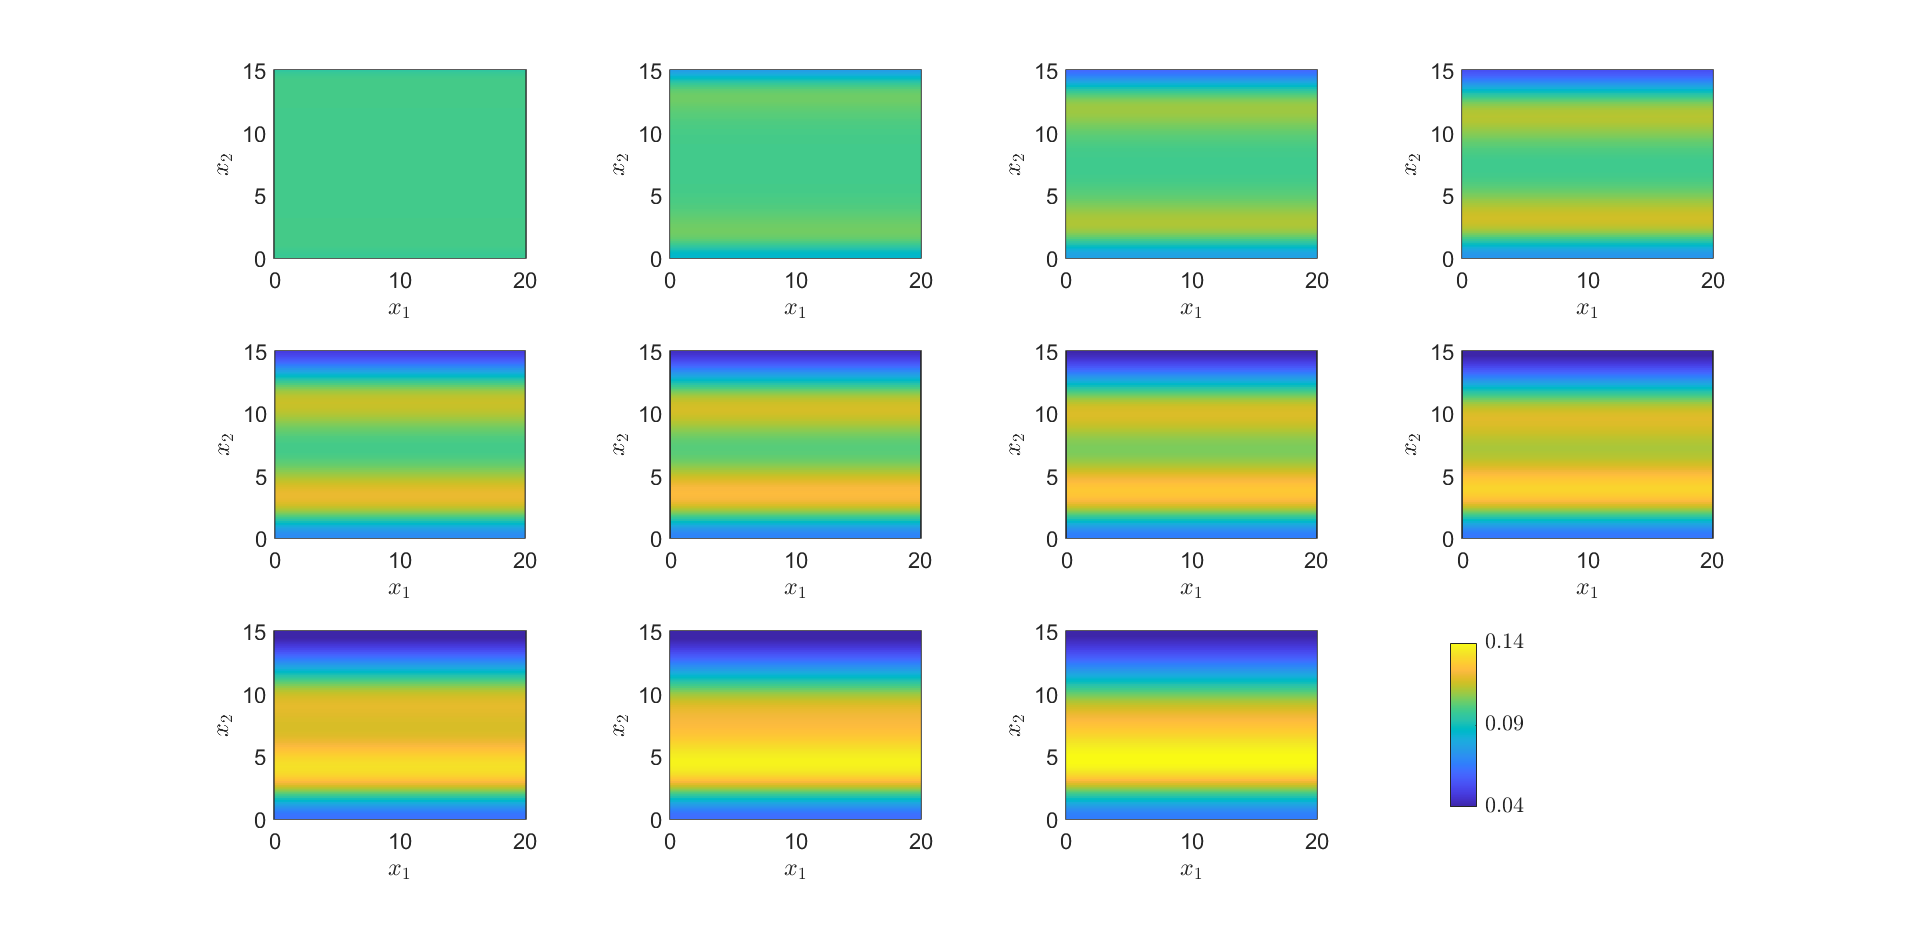
\includegraphics[scale=0.35]{rhoOptPeri8.png}
	\caption{Examples Section \ref{sec:PeriodicNoFlux3}: Optimal state $\rho$ in a periodic box, with $\kappa = 0$} 
	\label{F8a}
\end{figure}

\begin{figure}[h]
	\centering
	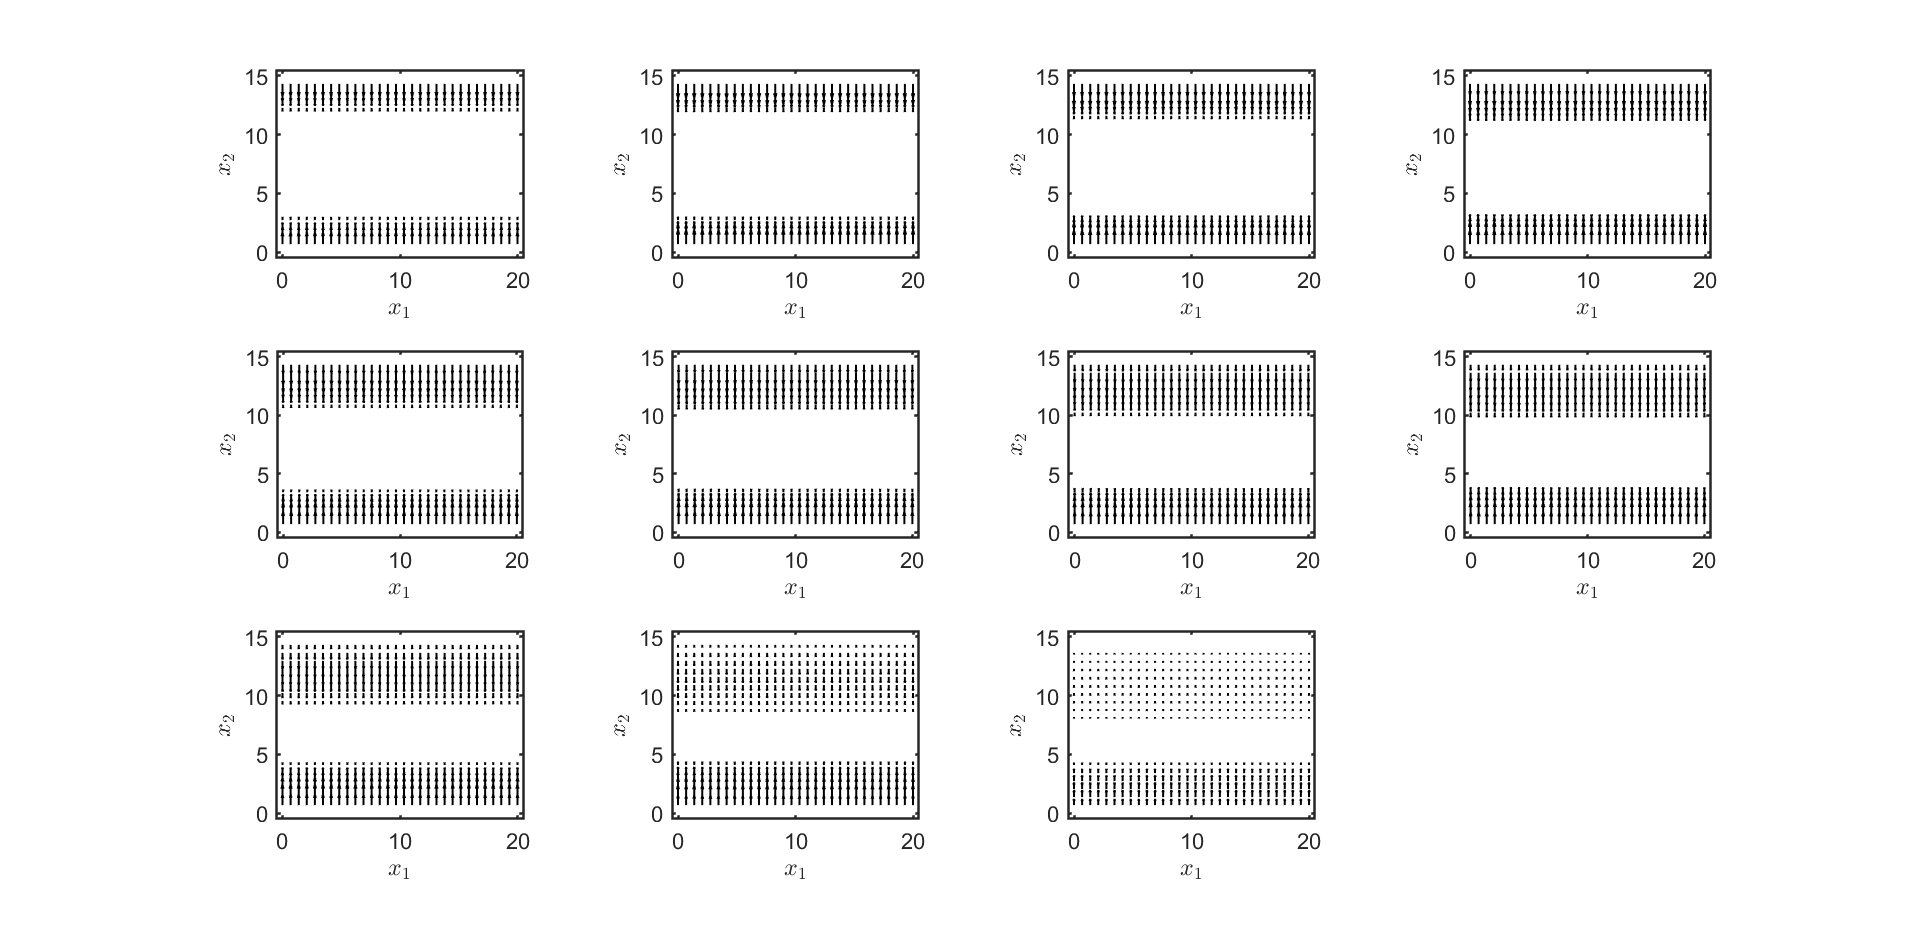
\includegraphics[scale=0.35]{ConOptPeri8.png}
	\caption{Examples Section \ref{sec:PeriodicNoFlux3}: Optimal control corresponding to optimal state in Figure \ref{F8a}.} 
	\label{F8b}
\end{figure}
\end{document}